\documentclass[a4paper, 12pt]{report}

\usepackage[dvipsnames]{xcolor}

%%%%%%%%%%%%%%%%%
% Set Variables %
%%%%%%%%%%%%%%%%%

\def\useItalian{0}  % 1 = Italian, 0 = English

\def\courseName{Quantum Computing}

\def\coursePrerequisites{TODO}

\def\book{"Quantum Computation and Quantum Information",\\Michael A. Nielsen, Isaac L. Chuang}

% \def\authorName{Simone Bianco}
% \def\email{bianco.simone@outlook.it}
% \def\github{https://github.com/Exyss/university-notes}
% \def\linkedin{https://www.linkedin.com/in/simone-bianco}

\def\authorName{Alessio Bandiera}
\def\email{alessio.bandiera02@gmail.com}
\def\github{https://github.com/aflaag-notes}
\def\linkedin{https://www.linkedin.com/in/alessio-bandiera-a53767223}

% Do not change

%%%%%%%%%%%%
% Packages %
%%%%%%%%%%%%

\usepackage{../../packages/Nyx/nyx-packages}
\usepackage{../../packages/Nyx/nyx-styles}
\usepackage{../../packages/Nyx/nyx-frames}
\usepackage{../../packages/Nyx/nyx-macros}
\usepackage{../../packages/Nyx/nyx-title}
\usepackage{../../packages/Nyx/nyx-intro}

\usepackage{qcircuit}

%%%%%%%%%%%%%%
% Title-page %
%%%%%%%%%%%%%%

\logo{../../packages/Nyx/logo.png}

\if\useItalian1
    \institute{\curlyquotes{\hspace{0.25mm}Sapienza} Università di Roma}
    \faculty{Ingegneria dell'Informazione,\\Informatica e Statistica}
    \department{Dipartimento di Informatica}
    \ifdefined\book
        \subtitle{Appunti integrati con il libro \book}
    \fi
    \author{\textit{Autore}\\\authorName}
\else
    \institute{\curlyquotes{\hspace{0.25mm}Sapienza} University of Rome}
    \faculty{Faculty of Information Engineering,\\Informatics and Statistics}
    \department{Department of Computer Science}
    \ifdefined\book
        \subtitle{Lecture notes integrated with the book \book}
    \fi
    \author{\textit{Author}\\\authorName}
\fi

\title{\courseName}
\date{\today}

% \supervisor{Linus \textsc{Torvalds}}
% \context{Well, I was bored\ldots}

\addbibresource{./references.bib}

%%%%%%%%%%%%
% Document %
%%%%%%%%%%%%

\begin{document}
\maketitle

% The following style changes are valid only inside this scope 
{
	\hypersetup{allcolors=black}
	\fancypagestyle{plain}{%
		\fancyhead{}        % clear all header fields
		\fancyfoot{}        % clear all header fields
		\fancyfoot[C]{\thepage}
		\renewcommand{\headrulewidth}{0pt}
		\renewcommand{\footrulewidth}{0pt}}

	\romantableofcontents
}

\introduction

%%%%%%%%%%%%%%%%%%%%%

\input{./chapters/intro.tex}
\chapter{Mathematical foundations}

Now that we have introduced some preliminary concepts in quantum mechanics and quantum computation, we can turn to the \tbf{mathematical foundations} that will allow us to develop a deeper understanding of the tools ahead. By the end of this chapter, we will be ready to state the postulates of quantum mechanics in a precise form. To prepare for that, we must first lay out several essential definitions and structures.

We will start our mathematical discussion with the definition of \tbf{scalar product} --- we will assume the definitions of vector space, basis and linear independence are already known by the reader.

\begin{frameddefn}{Scalar product}
	Given a scalar product vector space $V$, a \tbf{scalar product} $$\funcmap{\braket{\cdot , \cdot }}{V \times V}{\C}{(v, w)}{\braket{v,w}}$$ is a linear function that satisfies the following properties:

	\begin{itemize}
		\item $\forall u, v, w \in V, \alpha, \beta \in \C \quad \braket{u,\alpha v + \beta w} = \alpha \abk{u,v} + \beta \abk{u,w}$
		\item $\forall u, v \in V \quad \overline{\braket{u,v}} = \braket{v, u}$ --- where $\overline z$ is the conjugate of $z \in \C$
		\item $\forall u \in V \quad \braket{u, u} \ge 0$ and $\braket{u, u} = 0$ if and only if $u = 0$
	\end{itemize}
\end{frameddefn}

We see that the first property is the \tit{linearity} of the scalar product, while the second property is usually referred to as \tit{conjugate-symmetry}. Scalar products are also called \tit{inner product}, and are used to define many other tools on top of the vector space considered.

\begin{framedprop}{}
	For any scalar product vector space $V$, any scalar product satisfies the following property: $$\forall u, v, w \in V, \alpha, \beta \in \C \quad \braket{\alpha u + \beta v, w} = \overline \alpha \braket{u, w} + \overline \beta \braket{v, w}$$
\end{framedprop}

\begin{proof}
	By the properties of scalar product, the following holds
	\begin{equation*}
		\begin{split}
			\braket{\alpha u + \beta v, w} & = \overline{w, \alpha u + \beta v}                                                     \\
			                               & = \overline{\alpha \braket{w, u} + \beta \braket{w, v}}                                \\
			                               & = \overline \alpha \overline{\braket{w, u}} + \overline \beta \overline{\braket{w, v}} \\
			                               & = \overline \alpha \braket{u, w} + \overline \beta \braket{v, w}
		\end{split}
	\end{equation*}
\end{proof}

In particular, the scalar product that we are going to use for our purposes is defined as shown below.

\begin{frameddefn}{Hermitian product}
	Given a vector space $V$ defined over $\C$, the \tbf{Hermitian product} is defined as follows: $$\forall u, v \in \C^n \quad \braket{u, v} = \sum_{i = 1}^n{\overline{u_i} v_i}$$
\end{frameddefn}

\begin{framedprop}{}
	The Hermitian product is a scalar product.
\end{framedprop}

\begin{proof}
	It suffices to prove all the properties of scalar products provided in the definition. Then, we see that

	\begin{itemize}
		\item linearity can be proved as follows $$\braket{u, \alpha v + \beta w} = \sum_{i = 1}^n{\overline{u_i} (\alpha v_i + \beta w_i)} = \alpha\sum_{i = 1}^n{\overline{u_i} v_i} + \beta \sum_{i = 1}^n{\overline{u_i} v_i} = \alpha \braket{u, v} + \beta \braket{u, w}$$
		\item conjugate-symmetry can be shown as follows $$\overline{\braket{v, u}} = \overline{\sum_{i = 1}^n{\overline{v_i} u_i}} = \sum_{i = 1}^n{\overline{\overline{v_i} u_i}}= \sum_{i = 1}^n{v_i \overline{u_i}} = \braket{u, v}$$
		\item lastly, we have that $$\braket{u, u} = \sum_{ i= 1}^n{\overline{u_i}u_i} = \sum_{i = 1}^n{\abs{u_i}^2} \ge 0$$ and clearly it is equal to 0 if and only if $u = 0$
	\end{itemize}
\end{proof}

From now on, when we refer to a \curlyquotes{scalar product} we will refer to the Hermitian product.

We are finally ready to explain the \curlyquotes{braket} that we used from the beginning of the previous chapter. This notation was invented by the Nobel Prize in Physics \href{https://it.wikipedia.org/wiki/Paul_Dirac}{Paul Dirac}, and it works as follows: first, observe that our scalar product can be rewritten as follows $$\braket{u, v} = \rmat{\overline{u_1} \cdots \overline{u_n}} \rmat{v_1 \\ \vdots \\ v_n}$$ To be precise, this product would yield a $1 \times 1$ matrix, which can be interpreted as a scalar. Through Dirac notation, we will write $$\braket{u, v} = \braket{u | v}$$ where $\bra u$ is called \tbf{bra}, and $\ket v$ is called \tbf{ket} (as in \curlyquotes{bra-ket}). In other words, we have that $\ket v$ is just a regular column vector $v \in V$ $$\ket v = \rmat{v_1 \\ \vdots \\ v_n}$$ defined over some scalar product vector space $V$, while $\bra u$ is a \tit{linear map} that acts as follows: $$\funcmap{\bra \cdot}{V}{\overline V}{\rmat{u_1 \cdots u_n}}{\rmat{\overline{u_1} \cdots \overline{u_n}}}$$ We observe that from this very definition we can already see the power of the Dirac notation: by writing $$\bra u \cdot \ket v$$ we are writing the product between a row conjugated vector $u$ and a column vector $v$, which will ultimately yield $1 \times 1$ vector containing exatcly $\braket{u, v}$! Therefore, this allows us to write that $$\bra u \cdot \ket v = \braket{u|v}$$

\begin{framedthm}[label={cs ineq}]{Cauchy-Schwarz inequality}
	Given a scalar product vector space $V$, it holds that $$\forall u, v \in V \quad \abs{\braket{u|v}} \le \sqrt{\braket{u|u} \braket{v|v}}$$ where the equality holds if and only if $u$ and $v$ are linearly independent.
\end{framedthm}

Moreover, our scalar product induces a \tbf{norm}, which is defined as follows.

\begin{frameddefn}{Norm}
	Given a scalar product vector space $V$, the \tbf{norm} of a vector $v \in V$ is defined as follows $$\norm v = \sqrt{\braket{v|v}}$$
\end{frameddefn}

As usual, two vectors $u, v \in V$ are said to be \tbf{orthogonal} if $\braket{u|v} = 0$. This allows us to define orthonormal bases.

\begin{frameddefn}{Orthonormal basis}
	Given a scalar product vector space $V$, a basis $\{e_1, \ldots, e_n\}$ is said to be \tbf{orthonormal} if $$\forall i, j \in [n] \quad \braket{e_i | e_j} = \delta_{ij}$$ where $\delta_{ij} = \soe{ll}{1 & i = j \\ 0 & i \neq j}$ is called \tbf{Kronecker delta}.
\end{frameddefn}


Let's see the Dirac notation in action. Consider an orthonormal basis $\{e_1, \ldots, e_n\}$ for some scalar product vector space $V$; by definition, we know that we can write any vector $u \in V$ as follows $$u = \sum_{i = 1}^n{\alpha_i e_i}$$ for some coefficients $\alpha_1, \ldots, \alpha_n \in \C$. Now, we observe that for all $i \in [n]$
\begin{equation*}
	\begin{alignedat}{2}
		\braket{e_i|u} & = \abk{e_i\middle|\sum_{j = 1}^n{\alpha_j e_j}}                      & \\
		               & = \abk{e_i \middle|\alpha_1e_1 + \ldots + \alpha_n e_n}          & \\
		               & = \alpha_1 \braket{e_i|e_1} + \ldots + \alpha_n \braket{e_i|e_n} & \\
		               & = \sum_{j = 1}^n{\alpha_j\braket{e_i | e_j}}                     & \\
		               & = \sum_{j = 1}^n{\alpha_j \delta_{ij}}                           & \\
		               & = \alpha_i                                                       & \\
	\end{alignedat}
\end{equation*}
Indeed, with the scalar product we can compute the projection of $u$ onto the $i$-th vector of the basis. Hence, we can rewrite the first equation as follows: $$\ket u = \sum_{i = 1}^n{\alpha_i \ket{e_i}} = \sum_{i = 1}^n{\braket{e_i|u} \ket{e_i}}$$ In particular, we observe that $$\ket u = \sum_{i = 1}^n{\ket{e_i} \braket{e_i|u}} \implies I = \sum_{i = 1}^n{\ket{e_i} \bra{e_i}}$$ which is a famous identity in quantum mechanics called \tbf{resolution of the identity}. In particular, this identity directly implies the following useful property. As a final note, by the properties of scalar products we also have that $$\braket{v|u} = \bra{v} \sum_{i = 1}^n{\ket{e_i} \braket{e_i|u}} = \sum_{i= 1}^n{\braket{v|e_i} \braket{e_i|u}}$$

\begin{framedprop}{}
	Given a scalar product vector space $V$, it holds that $$\forall u, v, w \in V \quad \braket{u|v} \ket w = (\ket w \bra u) \ket v$$
\end{framedprop}

\section{Hilbert spaces}

Now that we covered Dirac notation, we can describe what are \tbf{Hilbert spaces} --- we will see why we care about this particular type of vector spaces later in the chapter. First, consider the following definitions.

\begin{frameddefn}{Weak convergence}
	Given a scalar product vector space $V$, and a vector sequence $\{v_m\}_{m \in \N}$ defined over $V$, we say that the sequence \tbf{converges weakly} to a vector $v \in V$ if $$\forall w \in V \quad \lim_{m \to + \infty}{\braket{v_m|w}} = \braket{v|w}$$
\end{frameddefn}

In other words, this type ocf convergence requires all projections of $v_m$ along any fixed direction $w$ to approach the projection of $v$. Differently, the next type of convergence is more strict.

\begin{frameddefn}{Strong convergence}
	Given a scalar product vector space $V$, and a vector sequence $\{v_m\}_{m \in \N}$ defined over $V$, we say that the sequence \tbf{converges strongly} to a vector $v \in V$ if $$\lim_{m \to + \infty}{\norm{v - v_m}} = 0$$
\end{frameddefn}

In fact, this type of convergence requires the actual vectors of the sequence to get close \tit{in norm} to $v$. We observe the following proposition.

\begin{framedprop}{}
	Given a scalar product vector space $V$, and a vector sequence $\{v_m\}_{m \in \N}$ defined over $V$, if the sequence converges strongly to some vector $v \in V$, it holds that

	\begin{itemize}
		\item the sequence also converges weakly
		\item the scalar products defined over $V$ are continuous, i.e. $$\forall u, v \in V \quad \braket{u|v} = \lim_{m \to + \infty}{\braket{u|v_m}}$$
	\end{itemize}
\end{framedprop}

\begin{frameddefn}{Cauchy sequence}
	Given a scalar product vector space $V$, and a vector sequence $\{v_m\}_{m \in \N}$ defined over $V$, we say that the sequence is a \tbf{Cauchy sequence} if it holds that $$\forall \varepsilon > 0 \quad \exists n_\varepsilon \in \N \quad \forall n, m > n_\varepsilon \quad \norm{v_n - v_m} < \varepsilon$$
\end{frameddefn}

For example, let's consider the space $\R^2$ equipped with the Euclidean norm $$\norm v =  \sqrt{x^2 + y^2}$$ Then, if we consider the following vector sequence $$\cbk{\rmat{\tfrac{1}{m} \\ \vdots \\ \tfrac{1}{m}}}_{m \in \N}$$ we see that for any distinct $m, n$ it holds that $$\norm{v_m - v_n} = \sqrt{\rbk{\dfrac{1}{m} -\dfrac{1}{n}}^2 + \rbk{\dfrac{1}{m} -\dfrac{1}{n}}^2} = \sqrt 2 \abs{\dfrac{1}{m} -\dfrac{1}{n}}$$ Therefore, for any $\varepsilon > 0$ it suffices to take any $N > \dfrac{2 \sqrt 2}{\varepsilon}$ such that $$\forall m, n > N \quad \norm{v_m - v_n} < \varepsilon$$

We are finally ready to define Hilbert spaces.

\begin{frameddefn}{Hilbert space}
	A \tbf{Hilbert space} is a \tit{complete} scalar product vector space, i.e. it is a vector space

	\begin{itemize}
		\item equipped with a scalar product
		\item such that every Cauchy sequence converges strongly to an element in the space.
	\end{itemize}
\end{frameddefn}

For example, the space $\R^n$ is a Hilbert space. Indeed, since every finite vector space of size $n$ is isomporphic to $\R^n$, we can immediately derive the following proposition.

\begin{framedprop}{}
	Finite-dimensional vector spaces are always complete.
\end{framedprop}

\subsection{Linear operators}

Given a Hilbert space $\mathcal H$, we can define \tbf{operators} --- which are nothing but linear maps.

\begin{frameddefn}{Adjoint operator}
	Given a Hilbert space $\mathcal H$, and an operator $A$, the \tbf{adjoint} operator of $A$, denoted with $A^\dag$, is a linear map that satisfies the following property $$\forall u, v \in \mathcal H \quad \braket{u|A^\dag v} = \braket{Au|v}$$ We say that an operator $A$ is \tbf{self-adjoint}, or \tit{Hermitian}, if and only if $A = A^\dag$.
\end{frameddefn}

For instance, the following matrix $S = \rmat{1 & 0 \\ 0 & i}$ is a linear operator whose adjoint is $S^\dag = \rmat{1 & 0 \\ 0 & -i}$. In fact, we have that $$\braket{u|S^\dag v} = \rmat{\overline{u_1} & \overline{u_2}} \rmat{1 & 0 \\ 0 & -i} \rmat{v_1 \\ v_2} = \rmat{\overline{u_1} & \overline{u_2}} \rmat{v_1 \\ -iv_2} = \overline{u_1}v_1 - i\overline{u_2}v_2$$ and since $$Su = \rmat{1 & 0 \\ 0 & i}\rmat{u_1 \\ u_2} = \rmat{u_1 \\ iu_2} \implies \bra{Su} = \rmat{\overline{u_1} & \overline{i u_2}}$$ but because $\overline{iu_2} = \overline i \cdot \overline{u_2} = -i \overline{u_2}$ this implies that $$\braket{Su |v} = \rmat{\overline{u_1} & -i\overline{u_2}} \rmat{v_1 \\ v_2} = \overline{u_1}v_2 - i\overline{u_2}v_2$$

\begin{framedprop}[label={adj prop}]{}
	For any adjoint operators $A, B$ defined over some Hilbert space $\mathcal H$, it holds that

	\begin{enumerate}
		\item $(AB)^\dag = B^\dag A^\dag$
		\item for any scalar $z$ it holds that $(zA)^\dag = \overline z A^\dag$
		\item $(A^\dag)^\dag = A$
		\item $(A + B)^\dag = A^\dag + B^\dag$
	\end{enumerate}
\end{framedprop}

How do we evaluate the adjoint of a given operator?

\begin{framedprop}[label={conj transp}]{}
	Given an operator $A$ defined over a scalar product vector space, it holds that $$a_{ij}^\dag = \overline{a_{ji}}$$
\end{framedprop}

This property is incredibly useful, because it implies that the adjoint operator of $A$ is its transposed conjugate matrix. Most notably, due to the way we defined our scalar product, it holds that for any column vector $\ket x$ we have that $$\bra x = \ket x^\dag$$ which gives an intuition of the reason why we defined our scalar product as such.

\begin{frameddefn}{Positive operator}
	An operator $A$ defined over a scalar product vector space $\mathcal H$ is said to be \tbf{positive} if it holds that $$\forall v \in \mathcal H \quad \braket{v|Av} \ge 0$$
\end{frameddefn}

\begin{framedprop}[label={positive prop}]{}
	If an operator $A$ is positive, then it is Hermitian.
\end{framedprop}

\begin{proof}
	TODO \todo{la dimostrazione che ha scritto lui è sbagliata}
\end{proof}

% \begin{proof}
% 	Let $A$ be a positive operator, therefore $$\forall v \in \mathcal H \quad \braket{v|Av} \ge 0$$ We observe that if $\braket{v|Av} \ge 0$, this implicitly means that $\braket{v|Av}$ is a real value. This is important because then $$\forall v \in \mathcal H \quad \braket{v|Av} = \overline{\braket{v|Av}}$$ From this, we derive the following
% 	\begin{equation*}
% 		\begin{split}
% 			\forall v \in \mathcal H \quad \overline{\braket{v|Av}} & = \braket{v|Av}                  \\
% 			                                                        & = \braket{A^\dag v|v}            \\
% 			                                                        & = \overline{\braket{v|A^\dag v}}
% 		\end{split}
% 	\end{equation*}
% 	which implies that $$\forall v \in \mathcal H \quad \braket{v|Av} = \braket{v|A^\dag v}$$ Now, consider the following claim.
%
% 	\claim{
% 		If $\braket{x|z} = \braket{y|z}$ for all $z \in \mathcal H$, then $x = y$.
% 	}{
% 		Fix a vector $z \in \mathcal H$; we observe that
% 		\begin{equation*}
% 			\begin{split}
% 				     & \braket{x|z} = \braket{y|z}     \\
% 				\iff & \braket{x|z} - \braket{y|z} = 0 \\
% 				\iff & (\bra x - \bra y) \ket z = 0    \\
% 				\iff & \braket{x - y|z} = 0
% 			\end{split}
% 		\end{equation*}
% 		However, if this is true for every vector $z \in \mathcal H$ it means that the vector $x - y$ is orthogonal to every vector in $\mathcal H$, which must imply that $x - y$ is the 0 vector, thus $$x - y = 0 \iff x = y$$
% 	}
%
% 	From this claim, we have that $$\forall v \in \mathcal H \quad \braket{v|Av} = \braket{v|A^\dag v} \iff \braket{A^\dag v|v} = \braket{Av|v} \implies A^\dag v = Av$$ which implies that $A$ must be Hermitian.
% \end{proof}

At the beginning of the previous chapter we said that all quantum gates are \tit{unitary transformations}, but we did now provide a definition of unitary. Now we are ready to introduce it, and start to grasp why we are discussing Hilbert spaces.

\begin{frameddefn}{Unitary operators}
	Given a Hilbert space $\mathcal H$, and an operator $U$, we say that $U$ is \tbf{unitary} if it holds that $$UU^\dag = U^\dag U = I$$
\end{frameddefn}

In other words, $U$ is unitary if and only if its adjoint operator is also its inverse. An interesting characterization of unitary transformations is the following property.

\begin{framedprop}[label={unitary alt def}]{Unitary operators (alt. def.)}
	An operator $U$ defined over a Hilbert space $\mathcal H$ is unitary if and only if

	\begin{itemize}
		\item $U$ is surjective
		\item $\forall x, y \in \mathcal H \quad \braket{Ux|Uy} = \braket{x|y}$ or equivalently, if it holds that $$\forall x \in \mathcal H \quad \norm{Ux} = \norm x$$
	\end{itemize}
\end{framedprop}

\begin{proof}
	TODO \todo{TODO}
\end{proof}

In particular, we observe that the second property of this proposition is very interesting: the \tit{preservation of the scalar product}, i.e. the property for which $$\forall x, y \in \mathcal H \quad \braket{Ux|Uy} = \braket{x|y}$$ means that the operator $U$ does not change the geometric relationships between vectors --- i.e. their lengths and angles remain the same.

\begin{framedprop}[label={rows cols unit}]{}
	If $U$ is a unitary operator, then the rows and the columns of $U$ are orthonormal.
\end{framedprop}

\begin{proof}
	First, we prove that the rows and columns of $U$ are normalized.

	\claim[Claim 1]{
		The norm of the rows and the columns of $U$ is 1.
	}{
		By the previous proposition, we know that $$\forall x \in \mathcal H \quad \norm{Ux} = \norm x$$ and in particular, this must hold for the canonical basis as well. This means that $$\norm{Ue_i} = \norm{e_i} = 1$$ for any vector of the canonical basis $e_i$. Then, since $Ue_i$ is just the $i$-th column of $U$, this proves that each column of $U$ has norm1.

		To prove the same result for the rows, observe that by \cref{conj transp} it holds that $$U^\dag = \overline U ^T$$ and \todo{da finire boh come??}
	}

	Next, we show orthogonality of rows and columns.

	\claim[Claim 2]{
		The rows and columns of $U$ are orthogonal.
	}{
		By the preservation of the scalar product, we know that $$\forall x, y \in \mathcal H \quad \braket{Ux|Uy} = \braket{x|y}$$ and in particular, this must also hold for the canonical basis. This means that for any pair of vectors of the canonical basis we have that $$\forall i, j \quad \braket{Ue_i|Ue_j} = \braket{e_i|e_j} = \delta{ij}$$ which means that the rows and columnds of $U$ must be orthogonal. \todo{does it?}
	}

	The two claims together conclude the proof.
\end{proof}

\begin{framedprop}[label={unitary prod}]{}
	If $A$ and $B$ are two unitary operators, then $AB$ is a unitary operator.
\end{framedprop}

\begin{proof}
	Since $A$ and $B$ are unitary it holds that $$A ^\dag A = A A^ \dag = B ^ \dag B = B B^ \dag = I$$ Now, by \cref{adj prop} we have that $$(AB)^ \dag = B^\dag A^\dag$$ from which we conclude that $$(AB)^\dag(AB) = B^\dag A^\dag AB = B^\dag I B = B^\dag B = I$$
\end{proof}

\begin{frameddefn}{Normal operators}
	Given a Hilbert space $\mathcal H$, and an operator $A$, we say that $A$ is \tbf{normal} if it satisfies the following property $$A^\dag A = AA^\dag$$
\end{frameddefn}

Clearly, from their definition we immediately see that both self-adjoint and unitary operators are both normal.

Lastly, say that we know that how an operator $U$ acts on some input $\ket x$, and we want to derive $U$. How can we do this?

\begin{framedprop}[label={U constr}]{}
	For any operator $U$ in a Hilbert space $\mathcal H$, if $\mathcal B$ is a base of $\mathcal H$ it holds that $$U = \sum_{b \in \mathcal B}{U \ket b \bra b}$$
\end{framedprop}

\begin{proof}
	The formula derives directly from the resolution of the identity, and the linearity of operators of Hilbert spaces
	\begin{equation*}
		\begin{split}
			U & = U \cdot I                                      \\
			  & = U \cdot \sum_{b \in \mathcal B}{\ket b \bra b} \\
			  & = \sum_{b \in \mathcal B}{U \ket b \bra b}
		\end{split}
	\end{equation*}
\end{proof}

Therefore, if we know how $U$ acts component-wise, we can reconstruct the operator acting on the whole space as such.

To conclude this section, we introduce a definition that will be very useful in the next chapter.

\begin{frameddefn}{Trace}
	Given a matrix $A \in \C^{n \times n}$, its \tbf{trace} is defined as follows: $$\tr(A) := \sum_{i = 1}^n{a_{ii}}$$
\end{frameddefn}

In other words, the trace of a matrix is the sum of the elements on its diagonal.

\begin{framedprop}[label={trace tricks}]{}
	Given two matrices $A, B \in \C^{n \times n}$, it holds that

	\begin{enumerate}
		\item $\tr(AB) = \tr(BA)$, meaning that the trace is \tit{cyclic}
		\item $\tr(A + B) = \tr(A) + \tr(B)$, meaning that the trace is \tit{linear}
		\item $\forall z \in \C \quad \tr(zA) = z \tr(A)$
		\item $\tr(A) = \tr(UAU^\dag)$ if $U$ is unitary, meaning that the trace is \tit{invariant under unitary similarity transformation}
	\end{enumerate}
\end{framedprop}

In particular, we observe that the last property follow trivially from the cyclic property: $$\tr(UAU^\dag) = \tr(UU^\dag A) = \tr(I A) = \tr(A)$$ But perhaps most importantly, the following property holds.

\begin{framedprop}[label={trace prop}]{}
	Given a matrix $A \in \C^{n \times n}$, and a vector $\ket v$, it holds that $$\tr(A \ket v \bra v) = \braket{v|Av}$$
\end{framedprop}

\begin{proof}
	First, we observe that the definition of the trace can be rewritten in terms of the Dirac notation $$\tr(X) = \sum_{i = 1}^n{x_{ii}} = \sum_{i = 1}^n{\braket{e_i|X|e_i}}$$ From this equality, we conclude that
	\begin{equation*}
		\begin{split}
			\tr(A \ket v \bra v) & = \sum_{i = 1}^n{\braket{e_i|A|v} \braket{v|e_i}}             \\
			                     & = \sum_{i = 1}^n{\braket{\psi|e_i} \braket{e_i|A|v}}          \\
			                     & = \bra{v} \rbk{\sum_{i = 1}^n{\ket {e_i} \bra{e_i}}} A \ket v \\
			                     & = \braket{v|A|v}                                              \\
			                     & = \braket{v|Av}
		\end{split}
	\end{equation*}
\end{proof}

Most importantly, if we set $A$ to be the identity matrix, we obtain an interesting identity: $$\tr( \ket v \bra v) = \braket{v|v}$$ which should not come as a surprise anyway, since the elements on the diagonal of $\ket v \bra v$ as exactly the elements of the sum in the scalar product of $\braket{v|v}$. We will discuss the importance of this equality in later sections.

TODO \todo{show that the trace is indep of the chosen basis}

\section{Spectral theory}

Since unitary operators are linear maps, we are interested in their eigenvectors and eigenvalues --- which are defined as usual. First, let us recall some preliminary definitions.

\begin{frameddefn}{Non-degenerate eigenvalue}
	Given a matrix $A$, and an eigenvalue $\lambda$ of $A$, we say that $\lambda$ is \tbf{non-degenerate} if the associated eigenspace has dimension 1 (or equivalently, if it has only 1 associated eigenvector).
\end{frameddefn}

\begin{frameddefn}{$d$-fold degenerate eigenvalue}
	Given a matrix $A$, and an eigenvalue $\lambda$ of $A$, we say that $\lambda$ is $d$-fold degenerate if there are $d$ linearly independent eigenvectors $u_1, \ldots, u_d$ associated to $\lambda$.
\end{frameddefn}

In Dirac notation, if $\lambda$ is non-degenerate, we refer to the only eigenvector associated to $\lambda$ as $\ket \lambda$, indeed it holds that $$A \ket \lambda = \lambda \ket \lambda$$ Interestingly enough from this equation we can immediately derive the following equality as well $$\bra \lambda A^\dag = \overline \lambda \bra \lambda$$

The following theorem provides a characterization of the eigenvalues and eigenvectors of self-adjoint and unitary operators, which have surprisingly nice properties.

\begin{framedthm}[label={spectral thm}]{Spectral theorem}
	The following propositions hold:

	\begin{itemize}
		\item The eigenvalues of a self-adjoint operator are real values.
		\item The eigenvalues of a unitary operator are complex values of modulus 1.
		\item Eigenvectors of self-adjoint and unitary operators associated to different eigenvalues are orthogonal to each other.
	\end{itemize}
\end{framedthm}

Moreover, for finite-dimensional Hilbert spaces the following holds.

\begin{framedthm}[label={spectral thm 2}]{Spectral theorem for fin. Hilbert spaces}
	Given a finite-dimensional Hilbert space $\mathcal H$, and a normal operator $A$ defined over $\mathcal H$, the set of all eigenvectors of $A$ can be expanded to form an orthonormal basis for $\mathcal H$.
\end{framedthm}

In particular, to basis expansion can be achieve through the \tbf{Gram-Shmidt} in the each degenerate eigenspace of $A$ in order to produce an orthonormal set.

% We can rewrite this thorem as follows: if we denote with $u_{ij}$ the $j$-th eigenvector associated to the $i$-th eigenvalue of $A$, it holds that $$\forall v \in \mathcal H \quad v = \sum_{i = 1}^m{\sum_{j = 1}^{d_i}{\alpha_{ij} u_{ij}}}$$ where $d_i$ is the geometric multiplicity of the $i$-th eigenvalue of $A$. Indeed, we observe that $\dim \mathcal H = \sum_{i = 1}^m{d_i}$. Lastly, through the Dirac notation we can rewrite the formula as follows $$\forall v \in \mathcal H \quad \ket v = \sum_{i = 1}^m{\sum_{j = 1}^{d_i}{\braket{\lambda_{ij}|v} \ket{\lambda_{ij}}}}$$

\section{Projectors}

Next, we are going to discuss \tbf{projectors}, which are another very crucial pieces of quantum computation. We saw how scalar products are able to perform projection over desired direction, in fact we will use the Dirac notation to define precise operators for our purposes. But as always, first some preliminary definitions.

\begin{frameddefn}{Orthogonal space}
	Given a scalar product vector space $U$, and two linear subspaces $V, W \subset U$, we say that $V$ is orthogonal to $W$ if $$\forall v \in V, w \in W \quad \braket{v|w} = 0$$
\end{frameddefn}

Given a scalar product vector space $U$, and a linear subspace $V \subset U$, the \tbf{orthogonal complement} of $V$ is defined as follows: $$V^\bot := \{u \in U \mid \forall v \in v \quad \braket{u|v} = 0\}$$ In particular, we observe that if $U$ is finite-dimentional it holds that $V = U - V^\bot$ and that $(V^\bot)^\bot = V$.

\begin{frameddefn}{Topologically closed subspace}
	Given a Hilbert space $\mathcal H$, and a linear subspace $V \subset \mathcal H$, we say that $V$ is \tbf{topologically closed} if any sequence of vectors defined over $V$ converges in $V$.
\end{frameddefn}

Interestingly enough, given a topologically closed subspace $V \subset \mathcal H$ of some Hilbert space, we can write any vector $u \in V$ as the sum of two orthogonal vectors of $V$ and $V^\bot$, as follows. Let $\{f_1, \ldots, f_n\}$ be an orthonormal basis of $V$, and define the following vectors $$\forall u \in U \quad u_V := \sum_{i = 1}^n{\braket{f_i|v} f_i}$$ Then, if we call $$u_{V^\bot} := u - u_V$$, we see that
% \begin{equation*}
%     \begin{alignedat}{2}
%         \braket{u_V|u_{V^\bot}} &= \braket{u_V|u - u_V} & \\ 
%                                 &= \braket{u_V|u} - \braket{u_V|u_V} & \\ 
%                                 &= \braket{\sum_{i = 1}^n{\braket{f_i|u} f_i}|u} - \braket{u_V|u_V} & \\ 
%                                 &= \sum_{i = 1}^n{\braket{f_i|u} \braket{f_i|u}} - \braket{u_V|u_V} & \\ 
%                                 &= \sum_{i = 1}^n{\abs{\braket{f_i|u}}^2} - \braket{u_V|u_V} & \\ 
%                                 &= \sum_{i = 1}^n{\overline{\braket{f_i|u}} \braket{f_i|u}} & \quad (\mbox{since $\abs{z}^2 = z \cdot \overline z$}) \\ 
%                                 & = \sum_{i = 1}^n{\sum_{j = 1}^n{\overline{\braket{f_i|u}} \braket{f_j|u} \delta_{i j}}} & \quad (\mbox{since $\delta_{ij} = \braket{f_i|f_j}$})
%     \end{alignedat}
% \end{equation*}
TODO \todo{decommenta e finisci la formula} which indeed proves that $u_V$ and $u_{V^\bot}$ are orthogonal to each other.

With this observation, we can finally define the projector operators.

\begin{frameddefn}{Projector}
	Given a Hilbert space $\mathcal H$, and a closed subspace $V \subset \mathcal H$, the \tbf{projector} operator that projects any given vector $v \in \mathcal H$ onto $V$ is defined as follows: $$\funcmap{P_V}{\mathcal H}{V}{u}{u_V = \sum_{i = 1}^n{\braket{f_i|u} f_i}}$$ where $\{f_1, \ldots, f_n\}$ is an orthonormal basis of $V$.
\end{frameddefn}

Most importantly, given the map in the definition we have that the projector operator $P_V$ is defined as follows $$P_V := \sum_{i = 1}^n{\ket{f_i} \bra{f_i}}$$ Clearly, by definition of $u_{V^\bot}$ it holds that $$\funcmap{P_{V^\bot}}{\mathcal H}{V^\bot}{u}{u_{V^\bot} := u - u_V}$$ Moreover, since $P_V$ performs a projection, we have that $$\forall u \in \mathcal H \quad u \in V \iff P_Vu = u$$ and that $$\forall u \in \mathcal H \quad u \in V^\bot \iff P_V u = 0$$

\begin{framedthm}{characterization of projectors}
	Given a Hilbert space $\mathcal H$, an operator $P_V$ is the projector on some closed subspace $V \subset \mathcal H$ if and only if
	\begin{enumerate}
		\item $P_V^2 = P_V$, i.e. it is \tit{idempotent}
		\item $P_V^\dag = P_V$, i.e it is Hermitian
	\end{enumerate}
\end{framedthm}

\begin{proof}
	We first prove the direct implication. Suppose that $P_V$ is the projector of a vector space $V \subset \mathcal H$, meaning that $P_V$ can be written as $$P_V = \sum_{i = 1}^n \ket {f_i} \bra{f_i}$$ for some orthonormal basis $\{f_i\}_{i = 1}^n$ of $V$. Then, we observe that
	\begin{equation*}
		\begin{split}
			P_V^2 & = \rbk{\sum_{i = 1}^n \ket{f_i} \bra{f_i}} \rbk{\sum_{j = 1}^n \ket{f_j} \bra{f_j}} \\
			      & = \sum_{i = 1} ^n \sum_{j = n} \ket{f_i} \braket{f_i|f_j} \bra{f_j}                 \\
			      & = \sum_{i = 1}^n \sum_{j = n} \ket{f_i} \delta_{i, j} \bra{f_j}                     \\
			      & = \sum_{i = 1}^n \ket{f_i} \bra{f_i} \\ 
			      & = P_V
		\end{split}
	\end{equation*}
	which immediately proves the idempotency of $P_V$. To prove Hermiticity, we observe that for any vector $\ket v$ it holds that $$(\ket v \bra v)^\dag = \ket v \bra v$$ that together with \cref{adj prop} it implies that
	\begin{equation*}
		\begin{split}
			P_V^\dag & = \rbk{\sum_{i = 1}^n{\ket{f_i} \bra{f_i}}}^\dag \\
			         & = \sum_{i = 1}^n{(\ket{f_i} \bra{f_i})^\dag}     \\
			         & = \sum_{i = 1}^n{\ket{f_i} \bra{f_i}}            \\
			         & = P_V
		\end{split}
	\end{equation*}
	We prove the converse implication in \cref{converse proj}.
\end{proof}

Given a Hilbert space $\mathcal H$, and two topologically closed subspaces $V, W \subset \mathcal H$, we say that $P_V$ and $P_W$ are \tbf{orthogonal} if it holds that $V \bot W$. Now, fix a vector $u \in \mathcal H$; by definition $P_Vu$ is a vector that lies inside $V$, therefore it holds that $$P_W(P_Vu) = 0$$ since $V \bot W$, and by the same reasoning applied on $W$ first we conclude that $$P_WP_V = P_VP_W = \mathbf 0$$ where $\mathbf 0$ is the \tbf{zero operator} --- indeed, it is a zero matrix.

As a final note, if $A$ is an linear operator, and $\lambda$ is an eigenvalue of $A$, we denote with $P_\lambda$ the projector that projects vectors onto the eigenspace associated to $\lambda$.

\begin{framedprop}[label={projector sum}]{}
	If $P$ and $Q$ are two orthogonal projectors, then $P + Q$ is a projector.
\end{framedprop}

\begin{proof}
    Let $\{f_i\}_{i = 1}^n$ and $\{g_i\}_{i = 1}^n$ be the bases that define $$P := \sum_{i = 1}^n \ket{f_i}\bra{f_i} \quad \quad Q := \sum_{i = 1}^n \ket{g_i} \bra{g_i}$$ We observe that $P \bot Q$, which means that $$\forall i, j \in [1, n] \quad \braket{f_i|g_j} = 0$$ Then, we have that $$P + Q = \sum_{i = 1} ^n \ket{f_i} \bra{f_i} + \sum_{i = 1}^n \ket{g_i} \bra{g_i}$$ Then, by the previous theorem it suffices to show that $P + Q$ is both idempotent and Hermitian. To prove idempotency we see that
    \begin{equation*}
	\hspace{-0.3cm}
        \begin{alignedat}{2}
            (P + Q)^2 & =  \rbk{\sum_{i = 1}^n \ket{f_i} \bra{f_i} + \sum_{i = 1}^n \ket{g_i} \bra{g_i }} \rbk{ \sum_{j = 1}^n \ket{f_j} \bra{f_j} + \sum_{j = 1}^n \ket{g_j} \bra {g_j}} & \\ 
                      & = \sum_{i, j}\ket{f_i } \braket{f_i|f_j} \bra{f_j} + \sum_{i, j} \braket{f_i} \braket{f_i|g_j} \bra{g_j} + \sum_{i, j} \ket{g_i} \braket{g_i|f_j} \bra{f_j} + \sum_{i, j} \ket{g_i } \braket{g_i|g_j} \bra{g_j} & \\ 
                      & = \sum_{i, j}\ket{f_i } \delta_{i, j} \bra{f_j} + \sum_{i, j} \ket{g_i } \delta_{i, j } \bra{g_j} & \\ 
                      & = \sum_{i = 1}^n \ket{f_i} \bra{f_i} + \sum_{j = 1}^n \ket{g_j} \bra{g_j} & \\ 
                      & = P + Q
        \end{alignedat}
    \end{equation*}
    We observe that we used orthogonality to remove the inner sums in the third step. Moreover, Hermiticity can be easily proven by linearity of the adjoint:
    \begin{equation*}
        \begin{split}
            (P + Q)^\dag & = \rbk{\sum_{i = 1}^n \ket{f_i} \bra{f_i } + \sum_{i = 1}^n \ket{g_i} \bra{g_i } }^\dag\\ 
                         & = \sum_{i = 1}^n (\ket {f_i} \bra{f_i})^\dag + \sum_{i = 1}^n (\ket{g_i} \bra{g_i})^\dag \\
                         & = \sum_{i = 1}^n \ket {f_i} \bra{f_i}+ \sum_{i = 1}^n \ket{g_i} \bra{g_i} \\ 
                          & = P + Q
        \end{split}
    \end{equation*}
\end{proof}

The importance of the next theorem cannot be understated, and it will be used extensively throughout the notes to prove various results.

\begin{framedthm}[label={spectral decomp}]{Spectral decomposition}
	Given a Hilbert space $\mathcal H$, and a normal operator $A$ defined on $\mathcal H$ whose eigenvalues are $\lambda_1, \ldots, \lambda_n$, the matrix $A$ can be rewritten as follows: $$A = \sum_{i = 1}^n{\lambda_i P_{\lambda_i}}$$
\end{framedthm}

The theorem above is sometimes written in the following different form $$A = \sum_{i = 1}^n{\lambda_i \ket{\lambda_i} \bra{\lambda_i}}$$ which \tit{seems} to imply that $P_{\lambda_i} = \ket{\lambda_i} \bra{\lambda_i}$, i.e. the projector onto the $i$-th eigenspace of $M$ is $\ket{\lambda_i} \bra{\lambda_i}$. This is a \tit{slight} notation abuse, and an example will make it clear. Consider the following matrix: $$A = \rmat{2 & 0 & 0 \\ 0 & 2 & 0 \\ 0 & 0 & 5}$$ It is easy to see that the eigenvalues of $A$ are only 2 and 5, however 2 is $2$-fold degenerate! Indeed, by solving $$M \ket v = 2 \ket v$$ we get an eigenspace of dimension 2, and we can choose $\{\ket {e_1}, \ket {e_2}\}$ as orthonormal eigenbasis; similarly, we find that $\{\ket {e_3}\}$ is an eigenbasis of the second eigenspace of dimension 1. In the end, this means that
\begin{equation*}
	\begin{split}
		M & = 2 \ket 1 \bra 1 + 2 \ket 2 \bra 2 + 5 \ket 3 \bra 3 \\
		  & = 2 (\ket 1 \bra 1 + \ket 2 \bra 2) + 5 \ket 3 \bra 3 \\
		  & = 2 P_2 + 5 P_5                                       \\
	\end{split}
\end{equation*}
which clearly shows that, in general, $P_{\lambda_i} \neq \ket{\lambda_i} \bra{\lambda_i}$! We observe that this also matches the definition of projector provided at the beginning of the section $$P_V := \sum_{i = 1}^n{\ket{f_i} \bra{f_i}}$$ for some orthonormal basis $\{f_1, \ldots, f_n\}$ of $V$. In general, the notation $$A = \sum_{i = 1}^n{\lambda_i \ket{\lambda_i} \bra{\lambda_i}}$$ implies that if $\lambda$ is $d$-fold degenerate, then $\lambda$ is repeated $d$ times inside the sum.

\section{Tensor product}

\subsection{General definition}

The last operation that we need to introduce into our mathematical background is the \tbf{tensor product}. There are multiple ways to define the tensor product.

\begin{frameddefn}{Tensor product}
	Given two vector spaces $V$ and $W$ defined over the same field, the \tbf{tensor product} $V \otimes W$ is a vector space together with a bilinear map $$\func{\otimes}{V \times W}{V \otimes W}$$ such that for every vector space $X$, and a bilinear map $\func{f}{V \times W}{X}$ there exists a unique linear map $\func{\tilde f}{V \otimes W}{X}$ with $$f = \tilde f \circ \otimes$$
\end{frameddefn}

\begin{figure}[H]
	\centering
	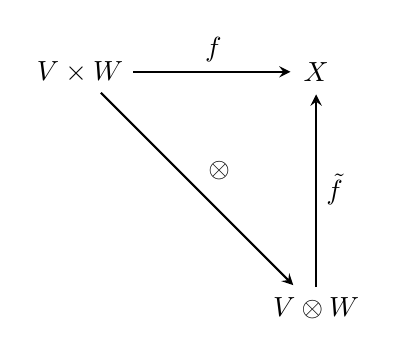
\begin{tikzpicture}[-,>=stealth,shorten >=1pt,auto,node distance=3cm, thick,main node/.style={scale=0.9,circle,draw,font=\sffamily\normalsize}]

		\node (1) []{$V \times W$};
		\node (2) [right of = 1]{$X$};
		\node (3) [below of = 2]{$V \otimes W$};

		\draw[->] (1) to node {$f$} (2);
		\draw[->] (1) to node {$\otimes$} (3);
		\draw[->] (3) to node[right] {$\tilde f$} (2);

		;
	\end{tikzpicture}
	\caption{The diagram of the definition above.}
\end{figure}


This definition is quite rigorous and dense, but a concrete example will make it clear. First, we recall that a function $f$ is \tbf{linear} if it holds that

\begin{itemize}
	\item $f(x + y) = f(x) + f(y)$
	\item $f (\alpha x) = \alpha f(x)$
\end{itemize}

Then, for a function to be \tbf{bilinear} (or \tit{multilinear}, in general) we require $f$ to be linear in both of its arguments:

\begin{itemize}
	\item $f(x + x', y) = f(x, y) + f(x', y)$
	\item $f(x, y + y') = f(x, y) + f(x, y')$
	\item $f(\alpha x, y) = \alpha f(x, y) = f(x, \alpha y)$
\end{itemize}

From this definition, we immediately point out that the tensor product $\otimes$ satisfies

\begin{itemize}
	\item $(v + v') \otimes w = v \otimes w + v' \otimes w$
	\item $v \otimes(w + w') = v \otimes w + v \otimes w'$
	\item $(\alpha v) \otimes w = v \otimes (\alpha w)$
\end{itemize}

We may call the first two as \tit{distributive properties}. Let's consider an example we already presented in the first chapter of the notes. At the start of our discussion we \curlyquotes{defined} the tensor product between two vectors $\rmat{a \\ b}$ and $\rmat{c \\ d}$ as follows $$\rmat{a \\ b} \otimes \rmat{c \\ d} := \rmat{ac \\ ad \\ bc \\ bd}$$ Now that we know what true definition is, we can apply it to understand why this is the case. First, we can assume that $\rmat{a \\ b}, \rmat{c \\ d} \in \R^2$ therefore $V = W = \R^2$. Therefore, our tensor product will have the signature $$\func{\otimes}{\R^2 \times \R^2}{\R^2 \otimes \R^2}$$ Now, we observe that the output space $V \otimes W$ is a vector space that has $$\mathcal B_{V \otimes W} := \{f_i  \otimes g_j \mid f_i \in \mathcal B_V, g_j \in \mathcal B_W\}$$ as a basis. In particular, this means that $$\mathcal B_{\R^2 \otimes \R^2} = \{e_1 \otimes e_1, e_1 \otimes e_2, e_2 \otimes e_1, e_2 \otimes e_2\}$$ is a basis for $\R^2 \otimes \R^2$. In fact, it is not diffcult to prove that $\R^4 \cong \R^2 \otimes \R^2$ by mapping the canonical basis of $\R^4$ to $\mathcal B_{\R^2 \otimes \R^2}$. Let $\varphi$ be the isorphism between the two. Then, by bilinearity of $\otimes$ we have that
\begin{equation*}
	\begin{split}
		\varphi \rbk{\rmat{a                                                                                                                               \\ b} \otimes \rmat{c \\ d}} & =   \varphi \rbk{(a e_1 + b e_2) \otimes (c e_1 + d e_2) }\\
		 & = \varphi \rbk{a c (e_1 \otimes e_1) + ad (e_1 \otimes e_2) + bc (e_2 \otimes e_1) + bd (e_2 \otimes e_2) }                                     \\
		 & = ac \cdot \varphi(e_1 \otimes e_1) + ad \cdot \varphi(e_1 \otimes e_2) + bc \cdot \varphi(e_2 \otimes e_1) + bd \cdot \varphi(e_2 \otimes e_2) \\
		 & = ac \cdot e_1 + ad \cdot e_2 + bc \cdot e_3 + bd \cdot e_4                                                                                     \\
		 & = \rmat{ac                                                                                                                                      \\ ad \\ bc \\ bd} \\
	\end{split}
\end{equation*}
Thus, in our example we have that $\tilde f = \varphi$ itself and $X = \R^4$, indeed $f = \varphi \circ \otimes$ is a function that maps pairs of two-dimensional vectors in $\R^2 \times \R^2$ into 4-dimensional vectors inside $\R^4$. This example also shows that the definition of tensor product does not depend on the choice of the vector space $X$, and for our purposes it is practical to choose a vector space that is isomporphic to $V \otimes W$.

What is the purpose of the tensor product in the first place? Given a vector space $V$, let $$\mbox{Functions}(V) := \{\func{f}{V}{K}\}$$ be the set of functions from $V$ to some other field $K$. It can be proven that this set forms a \tbf{vector space}. Then, the \tbf{tensor product} is the mathematical object that enables the following $$\mbox{Functions}(V \times W) = \mbox{Functions}(V) \otimes \mbox{Functions}(W)$$ This property is very useful as it allows to reason about functions on $V \times W$ not as a completely new object, but by studying it in terms of functions on $V$ and $W$ individually. In general, it allows to deal with objects that are \curlyquotes{more managable}. For instance, in our previous example the pair $\rbk{ \rmat{a \\ b}, \rmat{c \\ d}} \in \R^2 \times \R^2$ lies on a \tit{grid}, while an object $\rmat{ac \\ ad \\ bc \\ bd} \in \R^4$ is just a 4-dimensional vector.

Lastly, from the definition we observe that $$\dim(V \otimes W) = \dim V \cdot \dim W$$ indeed $V$ and $W$ can have different dimensions. For instance, a pair of vectors $(v, w) \in \R^2 \times \R^3$ lies in a 5-dimensional space, since $$\dim(V \times W) = \dim V + \dim W$$ however the tensor product generates a bigger space of size $$\dim (\R^2 \otimes \R^3) = \dim \R^2 \cdot \dim \R^3 = 2 \cdot 3 = 6$$ Indeed, we have that $$\R^2 \times \R^3 \cong \R^5 \quad \quad \R^2 \otimes \R^3 \cong \R^6$$

Consider any two vectors $v \in V$ and $w \in W$, and suppose that $n := \dim V$ and $m := \dim W$. Then, we can describe them in terms of $\mathcal B_V$ and $\mathcal B_W$, respectively, as follows: $$v = \sum_{i = 1}^n{\alpha_i f_i} \quad \quad w = \sum_{j = 1}^m{\beta_j g_j}$$ Then, by the distributive properties in the definition we have that
\begin{equation*}
	\begin{split}
		v \otimes w & = \rbk{\sum_{i = 1}^n{\alpha_i f_i}} \otimes \rbk{\sum_{j = 1}^m{\beta_j g_j}} \\
		            & = \sum_{i = 1}^n{\sum_{j = 1}^m{\alpha_i \beta_j (f_i \otimes g_j)}}
	\end{split}
\end{equation*}
which indeed is a vector that lies inside $V \otimes W$ since $(f_i \otimes g_j) \in \mathcal B_{V \otimes W}$. Then, if the basis of choice of the output set $X$ is the canonical basis, we observe that
\begin{equation*}
	\begin{split}
		\varphi(v \otimes w) & = \varphi \rbk{ \sum_{i = 1}^n{\sum_{j = 1}^m{\alpha_i \beta_j (f_i \otimes g_j)}}} \\
		                     & =  \sum_{i = 1}^n{\sum_{j = 1}^m{\alpha_i \beta_j \varphi(f_i \otimes g_j)}}        \\
		                     & =  \sum_{i = 1}^n{\sum_{j = 1}^m{\alpha_i \beta_j e_{(i - 1)m + j}}}                \\
		                     & = \rmat{\alpha_1 \beta_1                                                            \\ \alpha_1 \beta_2 \\ \vdots \\ \alpha_1 \beta_m \\ \alpha_2 \beta_1 \\ \vdots \\ \alpha_n \beta_m} \in \R^{n \cdot m} \\
	\end{split}
\end{equation*}
where the last column vector contains \tit{all} the pairs $(\alpha_i, \beta_j)$ --- note that $\R^{n \cdot m} \neq \R^{n \times m}$, as the latter denotes the space of real-valued matrices of dimension $n \times m$. Again, we underline that we arbitrarily chose the space $\R^{n \cdot m}$, but we could have chosen \tit{any} space of dimension $n \cdot m$ as output --- even $\R^{n \times m}$! A concrete example will clarify: consider two spaces $V = \R^2$ and $W = \R^{2 \times 2}$. Then, any element $v \in \R^2$ has the form $v = \rmat{a \\ b}$ while any matrix of $A \in \R^{2 \times 2}$ looks like $A = \rmat{c & d \\ e & f}$. If we want to compute $v \otimes A$, we can project it onto any space that has dimension $$\dim(\R^2 \otimes \R^{2 \times 2}) = \dim \R^2 \cdot \dim \R^{2 \times 2} = 2 \cdot 4 = 8$$ Here are some examples of the possible outputs of $v \otimes A$ depending on the choice of the output space: $$\rmat{ac \\ ad \\ ae \\ af \\ bc \\ bd \\ be \\ bf} \in \R^8 \quad \quad \rmat{ac & ad & ae & af \\ bc & bd & be & bf} \in \R^{2 \times 4} \quad \quad \rmat{ac & bc \\  ad & bd \\  ae & be \\ af & bf} \in \R^{4 \times 2}$$

\subsection{Kronecker product}

To conclude this chapter, let's look at the tensor product from the point of view of quantum computing. Until now, we presented examples regarding real-valued vectors, however, when talking about Hibert spaces in quantum computing we often need \tit{complex} values, as we already know. Consider a qubit $$\ket \psi = \alpha \ket 0 + \beta \ket 1$$ From this very formulation, we see that we are representing $\ket \psi$ under the \tbf{computational basis} $\{\ket 0, \ket 1\}$ we already encountered. However, since $\alpha, \beta \in \C$ this implies that $\ket \psi \in \C^2$. Now, consider a unitary operator acting on one qubit, for example the Hadamard gate $$H = \dfrac{1}{\sqrt 2} \rmat{1 & 1 \\ 1 & -1}$$ Our next goal is to compute $H \otimes H$. Clearly $H \in \C^{2 \times 2}$, therefore $H \otimes H \in \C^{2 \times 2} \otimes \C^{2 \times 2}$ which yields a space isomporphic to $\C^{16}$. However, since $H$ is a matrix it is not convenient to express the result inside $\C^{16}$, so we usually represent it inside $\C^{4 \times 4}$, which is still isomporphic to $\C^{16}$. After some calculations, we can show that $$H \otimes H = \dfrac{1}{2} \rmat{1 & 1 & 1 & 1 \\ 1 & -1 & 1 & -1 \\ 1 & 1 & -1 & -1 \\ 1  & -1 & -1 & 1}$$ However, we notice an interesting pattern in this result: this $4 \times 4$ matrix is essentially split into 4 sections that are \curlyquotes{multiples} of $H$ $$H \otimes H = \dfrac{1}{\sqrt 2} \rmat{1 \cdot H & 1 \cdot H \\ 1 \cdot H & -1 \cdot H}$$ In fact, for any two matrices $$A = \rmat{a & b \\ c & d} \quad \quad B = \rmat{e & f \\ g & h}$$ it holds that $$A \otimes B = \rmat{a B & b B \\ c B & d B } = \rmat{ae & af & be & bf \\ ag & ah & bg & bh \\ ce & cf & de & df \\ cg & ch & dg & dh}$$

We are finally ready to provide the formulation of the tensor product we will adopt for our purposes.

\begin{frameddefn}{Kronecker product}
	Given two matrices $A \in \mathbb F^{m \times n}$ and $B \in \mathbb F^{p \times q}$ defined over some field $\mathbb F$, the \tbf{Kronecker product} between $A$ and $B$ defines $A \otimes B$ as follows $$A \otimes B = \rmat{a_{11} B & \ldots & a_{1n}B \\ \vdots & \ddots & \vdots \\ a_{m1} B & \ldots & a_{mn} B} \in \F^{mp \times nq}$$
\end{frameddefn}

As an example, we observe that $$\rmat{a \\ b} \otimes \rmat{c \\ d} = \rmat{a \rmat{c \\ d} \\ b \rmat{c \\ d}} = \rmat{ac \\ ad \\ bc \\ bd}$$ which matches our previous results. From now on, we will assume that the output of any tensor product is in this form. Most importantly, through the Kronecker product the following property holds, which will be used extensively through these notes.

\begin{framedprop}[label={broken tensor}]{}
	For any field $\mathbb F$, given two matrices $A$ and $B$ and two vectors $v$ and $w$ such that $$A \in \mathbb F ^{m \times n} \quad B \in \mathbb F^{p \times q} \quad v \in \mathbb F^n \quad w \in \mathbb F^q$$ it holds that $$(A \otimes B)(v \otimes w) = Av \otimes Bw$$
\end{framedprop}

\begin{framedprop}[label={tensor adj}]{}
	For any two matrices $A$ and $B$ defined over a Hilbert space, it holds that $$(A \otimes B)^\dag = A^\dag \otimes B^\dag$$
\end{framedprop}

Another very important property of the tensor product is the way it behaves together with our scalar product.

\begin{framedprop}[label={tensor scalar}]{}
	For any four vectors $\ket a, \ket c \in \mathcal H_1$ and $\ket b, \ket d \in \mathcal H_2$ of two Hilbert spaces $\mathcal H_1$ and $\mathcal H_2$, it holds that $$\braket{a \otimes b| c \otimes d} = \braket{a|c} \braket{b|d}$$
\end{framedprop}

As a final note, if $U$ is a matrix (or a vector), we will write $$U^{\otimes n} = \underbrace{U \otimes \ldots \otimes U}_{n \ \mathrm{times}}$$ similar to the usual product $$U^{n} = \underbrace{U \cdot \ldots \cdot U}_{n \ \mathrm{times}}$$

\section{Exercises}

\begin{framedprob}{}
	Given $n$ qubits $\{q_i\}_{i = 1}^n$, show that $$\norm{\bigotimes_{i = 1}^n q_i} = 1$$
\end{framedprob}

\solution{
First, we observe that by \cref{tensor scalar} it immediately follows that for any set of vectors ${\{x_i\}^n}_{i = 1}$ and ${\{y_i\}^n}_{i = 1}$ it holds that $$\braket{a|b} = \prod_{i = 1}^n \braket{x_i|y_i}$$ From this observation, we conclude that it holds that $$\abk{ \bigotimes_{i = 1}^n x_i\middle|\bigotimes_{i = 1}^n y_i} = \prod_{i = 1}^n{\braket{x_i|y_i}}$$ From this observation, we conclude that

\begin{equation}
	\begin{alignedat}{2}
		\norm{\bigotimes_{i = 1}^n q_i}^2 & = \abk{\bigotimes_{i = 1}^n q_i \middle| \bigotimes_{i = 1}^n q_i} &                                            \\
		                                  & = \prod_{i = 1}^n \braket{q_i |q_i}                                                                             \\
		                                  & = \prod_{i = 1}^n \norm{q_i}^2                                     &                                            \\
		                                  & = \prod_{i = 1}^n 1                                                & \quad \quad (\mbox{since they are qubits}) \\
		                                  & = 1
	\end{alignedat}
\end{equation}
which ultimately concludes that $$\norm{\bigotimes_{i = 1}^n q_i} = 1$$
}

\begin{framedprob}{}
	Let $\{f_i\}_{i = 1}^n$ be an orthonormal basis of a vector space $V$, and fix a vector $u \in V$; then, consider $$u_V := \sum_{i = 1}^n{\braket{f_i|u} f_i}$$ Prove that the definition of $u_V$ does not depend on the choice of $\{f_i\}_{i = 1}^n$
\end{framedprob}

\solution{
By way of contradiction, suppose that there is an orthonormal basis $\{g_i\}_{i = 1}^n$ of $V$ such that $$\sum_{i = 1}^n \braket{f_i|u} \ket {f_i} \neq \sum_{i = 1}^n \braket{g_i|u} \ket{g_i}$$ Then, we have that
\begin{equation*}
	\begin{split}
		     & \sum_{i = 1}^n \braket{f_i|u} \ket {f_i} \neq \sum_{i = 1}^n \braket{g_i|u} \ket{g_i}        \\
		\iff & \sum_{i = 1}^n \ket {f_i}\braket{f_i|u}  \neq \sum_{i = 1}^n \ket{g_i}\braket{g_i|u}         \\
		\iff & \sum_{i = 1}^n \rbk{\ket{f_i} \braket{f_i|u} - \ket{g_i} \braket{g_i|u}} \neq 0              \\
		\iff & \sum_{i = 1}^n  \rbk {\ket{f_i} \bra{f_i} - \ket{g_i} \bra{g_i}} \ket u \neq 0               \\
		\iff & \rbk{\sum_{ i = 1}^n \ket{f_i} \bra{f_i} - \sum_{i = 1}^n \ket{g_i} \bra{g_i}} \ket u \neq 0 \\
		\iff & (P_V - P_V) \ket u  \neq 0                                                                   \\
		\iff & 0 \neq 0
	\end{split}
\end{equation*}
which is clearly a contradiction $\lightning$.
}

\begin{framedprob}[label={converse proj}]{}
	Show that if a matrix $P$ is both idempotent and Hermitian, it must be a projector.
\end{framedprob}

\solution{
    By Hermiticity, we know that $P$ admit a \nameref{spectral decomp}, i.e. $$P = \sum_{i = 1}^n{\lambda_i \ket{\lambda_i} \bra{\lambda_i}}$$ Now consider the following claim.

    \claim{
        If $P$ is an idempotent operator, its only possible eigenvalues are 0 and 1.
    }{
        By definition $v$ is an eigenvalue of $P$ associated to the eigenvector $\lambda$ if it holds that $$Pv = \lambda v$$ Hence, we observe that $$P^2 v = P (P v) = P (\lambda v) = \lambda Pv = \lambda(\lambda v) = \lambda^2 v$$ and therefore we have that $$\lambda^2 v = P^2 = Pv = \lambda v$$ which implies that $$\lambda^2v - \lambda v = 0 \iff (\lambda^2 - \lambda)v = 0$$ Finally, since $v$ is an eigenvector it holds that $v \neq 0$, therefore it must be that the last equation is true only if $$\lambda^2 - \lambda = 0 \iff \lambda = 0 \lor \lambda = 1$$
    }

    From this claim, we immediately obtain that each $\lambda_i$ is either 0 or 1, which means that its spectral decomposition can be written as $$P = \sum_j \ket{\lambda_j} \bra{\lambda_j}$$ for some non-zero eigenvalues $\lambda_j$ of $P$. This formulation concludes that $P$ is indeed a projector.
}

\begin{framedprob}{}
    Given a unitary matrix $U$, show that $U^{\otimes n}$ is still unitary.
\end{framedprob}

\solution{
    The property follows immediately from \cref{broken tensor} and \cref{tensor adj}, since
    \begin{equation*}
        \begin{split}
            U^{\otimes n} (U^{\otimes n})^\dag & = \rbk{ \bigotimes_{i = 1}^n U } \rbk{\bigotimes_{i = 1}^n U}^\dag \\ 
                                               & = \rbk{\bigotimes_{i = 1}^n U} \rbk{\bigotimes_{i = 1}^n U^\dag} \\ 
                                            & = \bigotimes_{i = 1}^n U U^\dag \\ 
                                            & = \bigotimes_{i = 1}^n I \\ 
                                             & = I
        \end{split}
    \end{equation*}
    The product $(U^{\otimes n})^\dag U^{\otimes n}$ can be proved analogously.
}

\begin{framedprob}{}
    Prove the triangular inequality.
\end{framedprob}

\solution{
    Consider two vectors $u$ and $v$ in some scalar product vector space; we must show that $$\norm{u + v} \le \norm u + \norm v$$ First, we observe that
    \begin{equation*}
        \begin{split}
            \norm{u + v}^2 & = \braket{u + v|u + v} \\ 
                           & = \braket{u + v|u} + \braket{u + v|v} \\ 
                           & = \braket{u|u} + \braket{v|u} + \braket{u|v} + \braket{v|v} \\ 
                           & = \norm u^2 + \braket{u|v} + \overline{\braket{u|v}} + \norm v^2
        \end{split}
    \end{equation*}
    Now, consider the following claim.

    \claim{
        For any complex number $z \in \C$ it holds that $z + \overline z = 2 \Re(z)$.
    }{
        The statement can be easily proven as follows: $$z + \overline z = \Re(z) + \Im(z) + \Re(z) - \Im(z) = 2 \Re(z)$$
    }

    From this claim, we can proceed as follows:
    \begin{equation*}
        \begin{alignedat}{2}
            \norm{u + v}^2 & = \norm u^2 + \braket{u|v} + \overline{\braket{u|v}} + \norm v^2 & \\ 
                           & = \norm u^2 + 2 \Re(\braket{u|v}) + \norm v^2 & \\ 
                           & \le \norm u^2 + 2 \abs{\braket{u|v}} + \norm v^2 & \\ 
                           & \le \norm u^2 + 2 \sqrt{\braket{u|u} \cdot \braket{v|v}} + \norm v^2 & \quad \quad (\mbox{by the \nameref{cs ineq}}) \\ 
                           & = \norm u^2 + 2 \sqrt{\braket{u|u}} \cdot \sqrt{\braket{v|v}} + \norm v^2 &  \\ 
                           & = \norm u^2 + 2 \norm u \norm v + \norm v^2 & \\ 
                            & = (\norm u + \norm v ) ^2 & \\ 
        \end{alignedat}
    \end{equation*}
    Then, since the vector norm is defined positive we ultimately conclude that $$\norm{u + v}^2 \le (\norm u + \norm v)^2 \implies \norm{u + v} \le \norm u + \norm v$$
}

\begin{framedprob}{}
    Prove the second property of the \nameref{spectral thm}, i.e. that the eigenvalues of a unitary operator are complex values of modulus 1.
\end{framedprob}

\solution{
    Let $U$ be a unitary transformation defined over some Hilbert space $\mathcal H$; by \cref{unitary alt def} we know that $$\forall x, y \in \mathcal H \quad \braket{Ux|Uy} = \braket{x|y}$$ Let $v \in \mathcal H$ be an eigenvector of $U$, i.e. there exists $\lambda \in \mbox{sp}(U)$ such that $$U \ket v = \lambda v$$ Then, we have that
    \begin{equation*}
        \begin{split}
            \braket{v|v} & = \braket{Uv|Uv} \\ 
                         & = \braket{\lambda v|\lambda v} \\
                            & = \overline \lambda \bra v \cdot \lambda \ket v \\ 
                            & = \abs{\lambda}^2 \braket{v|v}
        \end{split}
    \end{equation*}
    and since $v \neq 0$ because it is an eigenvector of $U$ we have that $$\braket{v|v} = \abs{\lambda}^2 \braket{v|v} \iff 1 = \abs{\lambda}^2 \implies \abs{\lambda} = 1$$
}

\begin{framedprob}{}
    Show that if an operator is unitary, it must be linear.
\end{framedprob}

\solution{
    Let $U$ be a unitary transformation defined over some Hilbert space $\mathcal H$; by \cref{unitary alt def} we know that $$\forall x, y \in \mathcal H \quad \braket{Ux|Uy} = \braket{x|y}$$ Fix three vectors $x, y, z \in \mathcal H$ and two complex values $\alpha, \beta \in \C$; then, by definition of scalar product we have that
    \begin{equation*}
        \begin{split}
            \braket{U(\alpha x + \beta y)|z} & = \braket{\alpha x + \beta y|U^\dag z} \\  
                                             & = \overline \alpha \braket{x|U^\dag z} + \overline \beta \braket{y| U^\dag z} \\ 
                                             & = \braket{\alpha Ux|z}  + \braket{\beta Uy|z} \\ 
                                              & = \braket{\alpha U x + \beta U y|z} \\
        \end{split}
    \end{equation*}
    Now, consider the following property of the scalar product.

	\claim{
		Given $x, y \in \mathcal H$, if  $\braket{x|z} = \braket{y|z}$ for all $z \in \mathcal H$, then $x = y$.
	}{
		Fix a vector $z \in \mathcal H$; we observe that
		\begin{equation*}
			\begin{split}
				     & \braket{x|z} = \braket{y|z}     \\
				\iff & \braket{x|z} - \braket{y|z} = 0 \\
				\iff & \braket{x - y|z} = 0
			\end{split}
		\end{equation*}
		However, if this is true for every vector $z \in \mathcal H$ it means that the vector $x - y$ is orthogonal to every vector in $\mathcal H$, which must imply that $x - y$ is the 0 vector, thus $$x - y = 0 \iff x = y$$
	}
        
        Then, from the previous observation we have $$\forall x, y, z \in \mathcal H , \alpha, \beta \in \C \quad \braket{U(\alpha x + \beta y)|z} = \braket{\alpha Ux + \beta Uy|z}$$ and this last claim concludes that $$U(\alpha x + \beta y) = \alpha U x + \beta U y$$ meaning that $U$ is indeed linear.
}

\chapter{Postulates of quantum mechanics}

TODO \todo{longer intro?}

Now that we defined Hilbert spaces and their operators in great detail, we can finally present we needed this mathematical foundations in order to progress: quantum mechanics is developed over Hilbert spaces with \tit{countable} bases, and quantum computing works with finite-dimensional Hilbert spaces. In particular, these are the four fundamental \tbf{postulates of quantum mechanics}.

\section{Postulates of quantum mechanics}

\subsection{First postulate}

\begin{framedpost}{State postulate}
	The state of a quantum system is completely described by a vector $\ket \psi$ in a Hilbert space $\mathcal H$.
\end{framedpost}

As we saw at the beginning of the previous chapter, $\ket \psi$ is always considered to be normalized. We observe that different physical systems of different types live in different Hilbert spaces.

\subsection{Second postulate}

\begin{framedpost}[label={time post}]{Time evolution postulate}
	A closed system evolves through time according to the \tbf{time-dependent Schrödinger equation (TDSE)}: $$i \hbar \dfrac{\diff}{\diff t} v(t) = Hv(t)$$
\end{framedpost}

We observe that the Schrödinger equation is a first-order linear differential equation, and it is composed by the following elements:

\begin{itemize}
	\item $v(t)$ which is the state vector at time $t$ (a vector in a Hilbert space)
	\item $H$ which is the system \tit{Hamiltonian}, a self-adjoint operator that describes the total energy of the system
\end{itemize}

The solution of the Schrödinger equation is $$v(t_1) = U(t_2, t_1)v(t_1)$$ where $U(t_2, t_1)$ is called \tbf{time-evaluation operator}, and it is defined as follows: $$U(t_2, t_1) = e^{-\tfrac{i}{\hbar}H(t_2 - t_1)}$$ (assuming $H$ does not depend on time). We recall that $H$ is a matrix, so we are raising $e$ to the power of a matrix, an operation that is defined by the power series of the exponential as follows: $$e^A = \sum_{n = 0}^\infty{\dfrac{A^n}{n!}}$$ What is interesting about this operator is that $U$ is \tbf{unitary}, and in order to show it is suffices to prove that $U^\dag = U^{-1}$. But how do we compute the adjoint of $U$? We observe that by the properties of the adjoint operation it holds that $$\rbk{e^A}^\dag = \rbk{\sum_{n = 0}^\infty{\dfrac{A^n}{n!}}}^\dag = \sum_{n = 0}^\infty{\dfrac{(A^n)^\dag}{n!}} = \sum_{n = 0}^\infty{\dfrac{(A^\dag)^n}{n!}} = e^{A^\dag}$$ which means that the adjoint of an exponential is the exponential of the adjoint. This suffices to prove that $$U^\dag = \rbk{e^{-\tfrac{i}{\hbar}H(t_2 - t_1)}}^\dag = e^{\rbk{-\tfrac{i}{\hbar}H(t_2 - t_1)}^\dag} = e^{\tfrac{i}{\hbar}H(t_2 - t_1)} = \rbk{e^{-\tfrac{i}{\hbar}H(t_2 - t_1)}}^{-1} = U^{-1}$$

This is a crucial characteristic for quantum mechanics: since $U$ is unitary, we know that it preserves the scalar product by \cref{unitary alt def}, therefore it also preserves \tbf{probabilities and norms}. This is why we say that evolution in quantum systems --- or \tit{quantum evolution}, for short --- is unitary. Indeed, the second postulate is sometimes formulated equivalently as follows.

\begin{framedpost}{Time evolution postulate (alt. ver.)}
	The evolution of a \tit{closed} quantum system is described by a \tit{unitary transformation}. That is, the state $\ket \psi$ of the system at time $t_1$ is related to the state $\ket{\psi'}$ of the system at time $t_2$ as follows $$\ket{\psi'} = U \ket \psi$$ where $U(t_2, t_1) = e^{-\tfrac{i}{\hbar}H(t_2 - t_1)}$.
\end{framedpost}

\subsection{Third postulate}

\begin{framedpost}[label={meas post}]{Measurement postulate}
	Every measurable (i.e. \tit{observable}) quantity corresponds to a self-adjoint operator on $\mathcal H$. In particular, given an observable $A$, and a state $v \in \mathcal H$, it holds that:
	\begin{itemize}
		\item the only possible results of measuring $A$ are one of its eigenvalues
		\item the probability of measuring eigenvalue $\lambda$ in state $v$ is given by $$\Pr[A = \lambda \mid v] = \braket{v|P_\lambda v}$$ where $P_\lambda$ is the linear map that projects $v$ onto the $\lambda$-eigenspace.
	\end{itemize}
\end{framedpost}

We can actually explain why we choose that particular scalar product to be the probability. Since by convention any quantum state is normalize, i.e. $\norm v = 1$, it holds that
\begin{equation*}
	\begin{split}
		1 & = \norm{v}^2                                                                 \\
		  & = \braket{v|v}                                                               \\
		  & = \abk{\sum_{i = 1}^m{P_{\lambda_i}v}\middle|\sum_{j = 1}^m{P_{\lambda_j}v}} \\
		  & = \sum_{i = 1}^m{\sum_{j = 1}^m{\braket{P_{\lambda_i}v|P_{\lambda_j}v}}}     \\
	\end{split}
\end{equation*}
Now, since each $P_{\lambda_i}$ is a projector, we know that when $i \neq j$ it holds that $P_{\lambda_i}P_{\lambda_j} = \mathbf 0$, therefore by Hermiticity of projectors we have that

\begin{itemize}
	\item if $i \neq j$ then $$\braket{P_{\lambda_i}v|P_{\lambda_j}v} =\braket{v|P_{\lambda_i}P_{\lambda_j}v} = \braket{v| \mathbf 0 v} = 0$$
	\item if $i = j$ then $$\braket{P_{\lambda_i}v|P_{\lambda_j}v} = \braket{P_{\lambda_i}v|P_{\lambda_i}v} = \norm{P_{\lambda_i}v}^2$$
\end{itemize}

Therefore, by adding only the non-zero terms we get that $$\sum_{i = 1}^m{\norm{P_{\lambda_i}v}^2} = 1$$ Hence, we define $$\Pr[A = \lambda_i \mid v] := \norm{P_{\lambda_i}v}^2$$ such that $$\Pr[A \mid v] = \sum_{i = 1}^m{\Pr[A = \lambda_i \mid v]} = \sum_{i = 1}^m{\norm{P_{\lambda_i}v}^2} = \norm{v}^2 = 1$$ which also means that our probabilities will add up to 1 automatically. Finally, we can rewrite this proability as follows (we will drop the index of the eigenvalue):
\begin{equation*}
	\begin{alignedat}{2}
		\Pr[A = \lambda \mid v] & = \braket{P_\lambda v | P_\lambda v}      &                               \\
		                        & = \braket{v | P_\lambda^\dag P_\lambda v} &                               \\
		                        & = \braket{v | P_\lambda^2 v}              & \quad (\mbox{by Hermiticity}) \\
		                        & = \braket{v | P_\lambda P_\lambda v}      &                               \\
		                        & = \braket{v | P_\lambda v}                &                               \\
	\end{alignedat}
\end{equation*}

This formulation was refined in 1926 by Max Born \cite{born}, when he derived the following property.

\begin{framedthm}[label={born rule}]{Born rule}
	The probability that a qubit $\ket \psi$ written in a basis $\{\lambda_i\}_{i = 1}^n$ collapses to a particular $\ket \lambda \in \{\lambda_i\}_{i = 1}^n$ when measured is $$\Pr[\mbox{measure}(\ket \psi = \ket \lambda)] = \abs{\braket{\psi|\lambda}}^2$$
\end{framedthm}

\begin{proof}
	By the \cref{spectral thm 2} it holds that the set of all the eigenvectors $\ket \lambda$ of any operator can be expanded to always form an orthonormal basis of the complete Hilbert space. Hence, the idea is to implicitly construct a self-adjoint operator $A$ whose eigenvalues are precisely the possible values in which $\ket \psi$ might collapse into. In other words, we want to construct a self-adjoint operator whose \nameref{spectral decomp} is exactly defined by $\{\lambda_1, \ldots, \lambda_n\}$ Hence, if $\ket \psi$ is defined as $$\ket \psi = \sum_{i = 1}^n {\alpha_n \ket{\lambda_i}}$$ we define the operator $$A_{\psi} = \sum_{i = 1}^n{\lambda_i \ket{\lambda_i} \bra{\lambda_i}}$$ Thus, the probability that by $\ket \psi$ it collapses to some $\ket \lambda \in\{\lambda_1, \ldots, \lambda_n\}$ can be rewritten as follows:
	\begin{equation*}
		\begin{alignedat}{2}
			\Pr[\mbox{measure}(\ket \psi = \ket \lambda)] & = \Pr[A_\psi = \lambda | \ket \psi]                &                                    \\
			                                              & = \braket{\psi|P_\lambda \psi}                     & \quad (\mbox{by \cref{meas post}}) \\
			                                              & = \braket{\psi|(\ket  \lambda \bra \lambda) \psi } &                                    \\
			                                              & = \braket{\psi|\ket \lambda \bra \lambda \psi}     &                                    \\
			                                              & = (\braket{\psi|\lambda})(\braket{\lambda|\psi})   &                                    \\
			                                              & = \abs{\braket{\psi|\lambda}}^2                    &                                    \\
		\end{alignedat}
	\end{equation*}
\end{proof}

For instance, if we have a superposition $$\ket \psi = \alpha \ket 0 + \beta \ket 1$$ and we want to know what is the probability that $\ket \psi$ collapses to $\ket 0$ after a measurement, we simply have that
\begin{equation*}
	\begin{split}
		\Pr[\mbox{measure}(\ket \psi = \ket 0)] & = \Pr[A_\psi = 0 | \ket \psi] \\
		                                        & = \abs{\braket{\psi|0}}^2     \\
	\end{split}
\end{equation*}
where the $A_\psi$ matrix is precisely: $$A_\psi = 0 \cdot P_0 + 1 \cdot P_1 = 0 \cdot \ket 0 \bra 0 + 1 \cdot \ket 1 \bra 1$$ This formulation of the probability of measurements will be used extensively for our purposes, and allows us to avoid the description of the matrix $A_\psi$ completely.

Before presenting to the next postulate, another very important operator that is frequently utilized in quantum mechanics is the \tbf{expected value} of a matrix. Given an observable $A$, we define the expected value of $A$ as the average eigenvector we may obtain after a measurement $$\Exp[A | v] = \sum_{i = 1}^m{\lambda_i \Pr[A = \lambda_i \mid v]}$$ We usually denote the expected value of the operator $A$ given that we are in state $\ket \psi$ as $\abk A_\psi$ (or $\abk A$ if the context is clear enough). Moreover, we have the following property.

\begin{framedprop}[label={exp of an op}]{Expected value of an operator}
	Given an Hermitian operator $A$, if the system is in state $\ket \psi$ it holds that $$\abk{A}_\psi = \braket{\psi|A \psi}$$
\end{framedprop}

\begin{proof}
	By \cref{meas post}, it follows that
	\begin{equation*}
		\begin{alignedat}{2}
			\abk{A}_\psi & = \Exp[A \mid \ket \psi]                                                    &                                                              \\
			             & = \sum_{i = 1}^m \lambda_i \Pr[A = \lambda_i \mid \ket \psi]                                                                               \\
			             & = \sum_{i = 1}^m \lambda_i \braket{\psi|P_{\lambda_i}|\psi}                 &                                                              \\
			             & = \bra \psi \left( \sum_{i = 1}^m \lambda_i P_{\lambda_i} \right) \ket \psi &                                                              \\
			             & = \bra \psi A \ket \psi                                                     & \quad \quad (\mbox{this is $A$'s \nameref{spectral decomp}}) \\
			             & = \braket{\psi| A \psi}                                                     &                                                              \\
		\end{alignedat}
	\end{equation*}
\end{proof}

Notably, \cref{trace prop} directly implies the following observation.

\begin{framedcor}{}
	Given an Hermitian operator $A$, if the system is in state $\ket \psi$ it holds that $$\abk{A}_\psi = \tr(A \ket \psi \bra \psi)$$
\end{framedcor}

\subsection{Fourth postulate}

\begin{framedpost}{Composite systems postulate}
	If system $A$ is defined over $\mathcal H_A$, and system $B$ is defined over $\mathcal H_B$, the total system lives in $$\mathcal H_{AB} = \mathcal H_A \otimes \mathcal H_B$$
\end{framedpost}

In other words, the last postulate states that the Hilbert space of a composite system is the tensor product of the Hilbert spaces of its subsystems.

Speaking of tensor products, when operators can be factored out into smaller operators of smaller systems we obtain linearity of expectations w.r.t. the tensor product.

\begin{framedprop}{}
	Given an operator $O$ that can be factored out as $O = A \otimes B$, if the current state $\ket \psi$ is not entangled it holds that $$\abk{O} = \abk{A} \cdot \abk{B}$$
\end{framedprop}

% \begin{proof}
% 	We need to show that $$\braket{\psi|O\psi} = \braket{\psi_A| A\psi_A} \cdot \braket{\psi_B|B\psi_B}$$ where $\ket \psi = \ket{\psi_A} \otimes \ket{\psi_B}$ which we know they exist because we are assuming that $\ket \psi$ is not entangled. Let the following be the spectral decompositions of $A$ and $B$, respectively $$A = \sum_{i = 1}^m{\lambda_i^A \ket{\lambda_i^A} \bra{\lambda_i^A}} \quad \quad B = \sum_{j = 1}^m{\lambda_j^B \ket{\lambda_j^B} \bra{\lambda_j^B}}$$ Then, by computing the tensor product between $A$ and $B$ we immediately obtain the spectral decomposition of $O$: $$O = A \otimes B = \sum_{i, j \in [m]}{\lambda_i^A\lambda_j^B (\ket{\lambda_i^A} \otimes \ket{\lambda_j^B})(\bra{\lambda_i^A} \otimes \bra{\lambda_j^B})}$$ Hence, the possible values $O$ might be observed into are all the products $\lambda_i^A \lambda_j^B$ for $i, j \in [m]$. Lastly, if we define $$\forall i, j \in [m] \quad \lambda_k = \lambda_{(i - 1)m + j}$$ it suffices to consider the definition of expected value:
%
% 	\begin{equation*}
% 		\begin{split}
% 			\braket{\psi|O\psi} & = \sum_{k = 1}^{m^2}{\lambda_k \Pr[O = \lambda_k \mid \ket \psi]}                                                                                            \\
% 			                    & = \sum_{k = 1}^{m^2}{\lambda_k \Pr[A \otimes B = \lambda_k \mid \ket {\psi_A} \otimes \ket{\psi_B}]}                                                         \\
% 			                    & = \sum_{k = 1}^{m^2}{\lambda_k \abs{\braket{\psi_A \otimes\psi_B | \lambda_k}}^2}                                                                            \\
% 			                    & = \sum_{i = 1}^m{\sum_{j = 1}^m{\lambda_i^A \lambda_j^B \abs{\braket{\psi_A \otimes \psi_B|\lambda_i^A \otimes \lambda_j^B}}^2}}                             \\
% 			                    & = \sum_{i = 1}^m{\sum_{j = 1}^m{\lambda_i^A \lambda_j^B \abs{\braket{\psi_A|\lambda_i^A} \cdot \braket{\psi_B|\lambda_j^B}}^2}}                              \\
% 			                    & = \sum_{i = 1}^m{\sum_{j = 1}^m{\lambda_i^A \lambda_j^B \abs{\braket{\psi_A|\lambda_i^A}}^2 \cdot \abs{\braket{\psi_B|\lambda_j^B}}^2}}                      \\
% 			                    & = \rbk{\sum_{i = 1}^m{\lambda_i^A \abs{\braket{\psi_A|\lambda_i^A}}^2}} \cdot \rbk{\sum_{j = 1}^m{\lambda_j^B \abs{\braket{\psi_B|\lambda_j^B}}^2}}          \\
% 			                    & = \rbk{\sum_{i = 1}^m{\lambda_i^A \Pr\sbk{A = \lambda_i^A| \ket{\psi_A}}}} \cdot \rbk{\sum_{j = 1}^m{\lambda_j^B  \Pr\sbk{B = \lambda_j^B | \ket {\psi_B}}}} \\
% 			                    & = \braket{\psi_A| A \psi_A} \cdot \braket{\psi_B|B \psi_B}                                                                                                   \\
% 		\end{split}
% 	\end{equation*}
% \end{proof}

\begin{proof}
	We need to show that
	\[
		\braket{\psi|O\psi} = \braket{\psi_A| A\psi_A} \cdot \braket{\psi_B|B\psi_B}
	\]
	where $\ket \psi = \ket{\psi_A} \otimes \ket{\psi_B}$, which we know exists because we are assuming that $\ket \psi$ is not entangled.

	Let the following be the spectral decompositions of $A$ and $B$, respectively:
	\[
		A = \sum_{i = 1}^m{\lambda_i^A P_{\lambda_i^A}}, \quad\quad B = \sum_{j = 1}^m{\lambda_j^B P_{\lambda_j^B}}
	\]
	Then, by computing the tensor product between $A$ and $B$, we immediately obtain the spectral decomposition of $O$:
	\[
		O = A \otimes B = \sum_{i, j \in [m]}{\lambda_i^A\lambda_j^B (P_{\lambda_i^A} \otimes P_{\lambda_j^B})}
	\]
	Hence, the possible values $O$ might be observed into are all the products $\lambda_i^A \lambda_j^B$ for $i, j \in [m]$. Lastly, if we define
	\[
		\forall i, j \in [m] \quad \lambda_k = \lambda_{(i - 1)m + j}
	\]
	it suffices to consider the definition of expected value:

	\begin{equation*}
		\begin{split}
			\braket{\psi|O\psi}
			 & = \sum_{k = 1}^{m^2} \lambda_k \Pr[O = \lambda_k \mid \ket \psi]                                                                                                                  \\
			 & = \sum_{i = 1}^m \sum_{j = 1}^m \lambda_i^A \lambda_j^B \Pr[A \otimes B = \lambda_i^A \lambda_j^B \mid \ket{\psi_A} \otimes \ket{\psi_B}]                                         \\
			 & = \sum_{i = 1}^m \sum_{j = 1}^m \lambda_i^A \lambda_j^B \braket{\psi_A \otimes \psi_B | P_{\lambda_i^A} \otimes P_{\lambda_j^B} | \psi_A \otimes \psi_B}                          \\
			 & = \sum_{i = 1}^m \sum_{j = 1}^m \lambda_i^A \lambda_j^B \left( \braket{\psi_A | P_{\lambda_i^A} | \psi_A} \cdot \braket{\psi_B | P_{\lambda_j^B} | \psi_B} \right)                \\
			 & = \sum_{i = 1}^m \left( \lambda_i^A \braket{\psi_A | P_{\lambda_i^A} | \psi_A} \sum_{j = 1}^m \lambda_j^B \braket{\psi_B | P_{\lambda_j^B} | \psi_B} \right)                      \\
			 & = \left( \sum_{i = 1}^m \lambda_i^A \braket{\psi_A | P_{\lambda_i^A} | \psi_A} \right) \cdot \left( \sum_{j = 1}^m \lambda_j^B \braket{\psi_B | P_{\lambda_j^B} | \psi_B} \right) \\
			 & = \braket{\psi_A| A \psi_A} \cdot \braket{\psi_B| B \psi_B}
		\end{split}
	\end{equation*}
\end{proof}

This result should not come as a surprise, since for any two distributions $X$ and $Y$ we know that $$\Exp[XY] = \Exp[X] \cdot \Exp[Y]$$ only if $X$ and $Y$ are \tbf{independent}. Indeed, by assuming that $O$ and $\ket \psi$ can be factorized, we are assuming that the two underlying subsystems $\mathcal H_A$ and $\mathcal H_B$ --- in which $\ket{\psi_A}$ and $A$,  and $\ket{\psi_B}$ and $B$ live, respectively --- are \curlyquotes{independent} in the sense that they are \tit{not entangled}!

\section{Density operators}

We have formulated quantum mechanics using state vectors and the four postulates described in the previous section. However an alternate formulation is possible using a tool known as the \tbf{density operator}, or \tit{density matrix}. This formulation will be mathematically equivalent to the state vector approach. However, before proceeding we need to revise some definitions we provided in the previous section.

\subsection{Generalization of the third postulate}

The postulates we have just presented are internally consistent, however, to proceed further we require additional clarification regarding the \nameref{meas post}. In particular, in the statement of this postulate we required that measurables are self-adjoint (i.e. Hermitian) operators. To be precise, this is a special case of a more general formalization of the Measurement postulate which we need to discuss.

\begin{framedpost}[label={gen meas post}]{General measurement postulate}
	Quantum measurements are described by a collection $\{M_m\}$ of \tit{measurement operators} acting on the state space of the system being measured --- the index $m$ refers to the measurement outcomes that may occur in the experiment. If the state of the quantum system is $\ket \psi$ immediately before the measurement, then the probability that result $m$ occurs is given by $$\Pr[m \mid \ket \psi] = \bra \psi M_m^\dag M_m \ket \psi$$ and the measurement operators satisfy the \tbf{completeness equation} $$\sum_{m}{M_m^\dag M_m} = I$$
\end{framedpost}

We observe that the completeness equation expresses the fact that probabilities of the outcomes sum to one:
\begin{equation*}
	\begin{split}
		\sum_{m}{\Pr[m \mid \ket \psi]} & = \sum_{m} {\bra \psi M_m^\dag M_m \ket \psi}     \\
		% & = \abk{\psi \middle| \sum_{m}{M_m^\dag M_m} \middle| \psi} \\
		                                & = \bra \psi \rbk{\sum_m {M_m^\dag M_m}} \ket \psi \\
		                                & = \braket{\psi|I|\psi}                            \\
		                                & = \braket{\psi|\psi}                              \\
		                                & = 1
	\end{split}
\end{equation*}

For instance, consider a single qubit $$\ket \psi = \alpha \ket 0 + \beta \ket 1$$ and suppose we want to measure it in the computational basis. The two measurement operators we require are precisely $$M_0 := \ket 0 \bra 0 \quad \quad M_1 := \ket 1 \bra 1$$ We observe that these two operators are \tit{projectors}, so they trivially satisfy the completeness equation
\begin{equation*}
	\begin{alignedat}{2}
		M_0^\dag M_0 + M_1^\dag M_1 & = M_0^2 + M_1^2 &                                        \\
		                            & = M_0 + M_1     & \quad \quad (\mbox{resolution of $I$}) \\
		                            & = I             &                                        \\
	\end{alignedat}
\end{equation*}
Then, the probability of obtaining 0 from measuring $\ket \psi$ is $$\Pr[0 \mid \ket \psi] = \braket{\psi|M_0^\dag M_0|\psi} = \braket{\psi|M_0|\psi} = \abs{\alpha}^2$$ and similarly we ge that $\Pr[1 \mid \ket \psi] = \abs{\beta}^2$, as we would expect.

So, what is the connection with the initial version of the third postulate we originally provided? A special case of the General measurement postulate when the measurements are \tit{projective measurements}, i.e. measurements described by Hermitian operators. Indeed, for many applications of quantum computation and quantum information in general we are concerned primarily with projective measurements. By requiring that observables are Hermitian operators the third postulate reduces to the formulation we provided in the previous section, because any observable $M$ would have a spectral decomposition of $$M = \sum_{m}{m P_m}$$ which immediately implies that $$\Pr[m \mid \ket \psi] = \braket{\psi|P_m \psi}$$ as defined earlier.

\subsection{Postulates through density operators}

We can now introduce the \tbf{density operator} discussed at the beginning of the section. First, we describe the context. Consider a quantum system, and suppose that it is in one of a number of states $\ket{\psi_1}, \ldots, \ket{\psi_N}$. Each $\ket{\psi_i}$ is associated with a probability $p_i$ that the system is in the $i$-th state. We call $$\{p_i, \ket {\psi_i}\}_{i = 1}^N$$ an \tbf{ensable of states}. Then, we the following definition.

\begin{frameddefn}{Density operator}
	Given a quantum system described by the ensamble $\{p_i, \ket{\psi_i}\}_{i = 1}^N$, the \tbf{density operator} of the system is defined as follows $$\rho := \sum_{i = 1}^N{p_i \ket{\psi_i} \bra{\psi_i}}$$
\end{frameddefn}

We observe that $\rho$ is a matrix, and this is the reason why it is interchangeably called \tit{density matrix}. Nevertheless, this matrix is important because it turns out that all the postulates of quantum mechanics we presented so far can be reformulated equivalently in terms of the density operator.

Suppose that we have closed quantum system described by some ensamble $\{p_i, \ket{\psi_i}\}_{i = 1}^N$ that unitarily evolves following the unitary operator $U$ described earlier $$U(t_2, t_1) = e^{-\tfrac{i}{\hbar}H(t_2 - t_1)}$$ This means that the system is in state $\ket{\psi_i}$ with probability $p_i$, and after the evolution has occurred the system will be in the state $U \ket{\psi_i}$ still with probability $p_i$. More specifically, we have that $$\ket{\psi_i} \xlongrightarrow{U} U \ket{\psi_i}$$ which also directly implies that $$(\ket{\psi_i})^\dag = \bra{\psi_i} \xlongrightarrow{U} (U \ket{\psi_i})^\dag = \bra{\psi_i} U^\dag$$ Therefore, after the system has evolved we must \tit{update} its density operator by applying $U$ to each $\ket{\psi_i}$ --- we don't know in which state the system is in with certainty by the rules of quantum mechanics, so we take into account all of the possible \todo{this explaination sucks find a better reason tbh} $\ket{\psi_i}$ $$\rho = \sum_{i = 1}^N{p_i \ket{\psi_i} \bra{\psi_i}} \xlongrightarrow{U} \sum_{i = 1}^N{p_i U \ket{\psi_i} \bra{\psi_i} U^\dag} = U \rho U^\dag$$ Not surprisingly, this shows that by linearity we just need to apply $U$ (and $U^\dag$) to the matrix directly in order to consider all the evolutions. The function that maps $$\rho \mapsto U \rho U^\dag$$ is called \tbf{superoperator}.

Measurements can be also easily described through the density operator. Consider the \nameref{gen meas post}, and suppose we perform a measurement described by measurement operators $M_m$. If the initial state was $\ket{\psi_i}$, then we have that
\begin{equation*}
	\begin{alignedat}{2}
		\Pr[m|\ket{\psi_i}] & = \braket{\psi_i|M_m^\dag M_m|\psi_i}         &                                           \\
		                    & = \tr(M_m^\dag M_m \ket{\psi_i} \bra{\psi_i}) & \quad \quad (\mbox{by \cref{trace prop}}) \\
	\end{alignedat}
\end{equation*}
Then, thanks to \cref{trace tricks}, by computing the total probability we obtain that
\begin{equation*}
	\begin{split}
		\Pr[m] & = \sum_{i = 1}^N{p_i\Pr[m\mid \ket{\psi_i}]}                           \\
		       & = \sum_{i = 1}^N{p_i \tr(M_m^\dag M_m \ket{\psi_i} \bra{\psi_i})}      \\
		       & = \sum_{i = 1}^N{\tr(p_i M_m^\dag M_m \ket{\psi_i} \bra{\psi_i})}      \\
		       & = \tr \rbk{\sum_{i = 1}^N{p_i M_m^\dag M_m \ket{\psi_i} \bra{\psi_i}}} \\
		       & = \tr \rbk{M_m^\dag M_m \sum_{i = 1}^N{p_i \ket{\psi_i} \bra{\psi_i}}} \\
		       & = \tr(M_m^\dag M_m \rho)                                               \\
	\end{split}
\end{equation*}

TODO \todo{skipping rho m, if needed put it here and add what it is needed in the general meas post}

This shows that the basic postulates of quantum mechanics related to unitary evolution and measurement can be rephrased in terms of density operators. However, we can do better: we will proivde a characterization of the density operator that does not rely on the idea of state vectors \tit{at all}. But first, as usual, we need some definitions. When a quantum system is an a known exact state $\ket \psi$, the system is said to be in a \tbf{pure state}, and in this case its density matrix operator is simply $$\rho = \ket \psi \bra \psi$$ Otherwise, if the state is now known and the system is described by an ensamble of states, we say that $\rho$ is in a \tbf{mixed state}. More specifically, we can distinguish between pure and mixed states as follows.

\begin{framedprop}{}
	If a system is in a pure state it holds that $\tr(\rho^2) = 1$, otherwise if it is in a mixed state it holds that $\tr(\rho^2) < 1$.
\end{framedprop}

\begin{proof}
	TODO \todo{da fare}
\end{proof}

We can finally present the characterization of density operators we anticipated.

\begin{framedthm}{Density operators characterization}
	Given a system described by the ensamble $\{p_i, \ket{\psi_i}\}_{i = 1}^N$, an operator $\rho$ is the density operator of the system if and only if

	\begin{itemize}
		\item $\rho$ is positive
		\item $\tr(\rho) = 1$
	\end{itemize}
\end{framedthm}

\begin{proof}
	We first prove the first implication. Consider the density operator $$\rho = \sum_{i = 1}^N{p_i \ket{\psi_i} \bra{\psi_i}}$$ Fix an arbitrary $\ket v \in \mathcal H$; then, we get that:
	\begin{equation*}
		\begin{split}
			\braket{v|\rho v} & = \braket{v|\rho|v}                                                 \\
			                  & = \bra v \rbk{\sum_{i = 1}^N{p_i \ket{\psi_i} \bra{\psi_i}}} \ket v \\
			                  & = \sum_{i = 1}^N{p_i \braket{v|\psi_i} \braket{\psi_i| v}}          \\
			                  & = \sum_{i = 1}^N{p_i \abs{\braket{v|\psi_i}}^2}                     \\
			                  & \ge 0
		\end{split}
	\end{equation*}
	This proves that $\rho$ is positive. For the second statement, by the property of the trace proved in \cref{trace tricks} and \cref{trace prop}, we obtain that
	\begin{equation*}
		\begin{split}
			\tr(\rho) & = \tr \rbk{\sum_{i = 1}^N{p_i \ket{\psi_i} \bra{\psi_i}}} \\
			          & = \sum_{i = 1}^N{p_i \tr(\ket{\psi_i} \bra{\psi_i})}      \\
			          & = \sum_{i = 1}^N{p_i \braket{\psi_i|I\psi_i}}             \\
			          & = \sum_{i = 1}^N{p_i \braket{\psi_i|\psi_i}}              \\
			          & = \sum_{i = 1}^n{p_i}                                     \\
			          & = 1
		\end{split}
	\end{equation*}

	Now we can proceed to prove the converse implication. Suppose that $\rho$ is any operator that satisfies the conditions of the statement. In particular, since $\rho$ is positive by \cref{positive prop} we know that $\rho$ is Hermitian, which implies that it admits a spectral decomposition TODO \todo{da finire, troppo noioso}
\end{proof}

\begin{framedprop}{Convexity of density matrices}
	Given density matrices $\rho_1, \ldots, \rho_n$ and probabilities $p_1, \ldots, p_n$ it holds that $\sum_{i = 1}^N{p_i \rho_i}$ is a density matrix.
\end{framedprop}

\begin{proof}
	TODO \todo{da fare}
\end{proof}

Given all we just discussed, we can finally rephrase the postulates through the density operator.

\begin{framedpost}{State postulate (density operator)}
	Associated to any isolated physical system is a Hilbert space known as the \tit{state space} of the system, and the system is completely described by its \tit{density operator}, i.e. any positive operator $\rho$ with trace one acting on the state space of the system.
\end{framedpost}

\begin{framedpost}{Time evolution postulate (density op.)}
	The evolution of a \tit{closed} quantum system is described by a \tit{unitary transformation}, i.e. the state $\rho$ of the system at time $t_1$ is related to the state $\rho'$ of the system at time $t_2$ as follows $$\rho' = U \rho U^\dag$$ where $U(t_2, t_1) = e^{-\tfrac{i}{\hbar}H(t_2 - t_1)}$.
\end{framedpost}

\begin{framedpost}{General measurement postulate (dens. op.)}
	Quantum measurements are described by a collection $\{M_m\}$ of \tit{measurement operators} acting on the state space of the system being measured --- the index $m$ refers to the measurement outcomes that may occur in the experiment. If the state of the quantum system is $\rho$ immediately before the measurement, then the probability that result $m$ occurs is given by $$\Pr[m \mid \ket \psi] = \tr(M_m^\dag M_m \rho)$$ and the measurement operators satisfy the \tbf{completeness equation} $$\sum_{m}{M_m^\dag M_m} = I$$
\end{framedpost}

TODO \todo{ex: do the projection one}

\begin{framedpost}{Composite system postulate (dens. op.)}
	The sate space of a composite physical system is the tensor product of the state spaces of the component physical systems. That is, given $n$ systems such that the $i$-th system is in state $\rho_i$, the joint state of the total system is $$\rho = \bigotimes_{i = 1}^n{\rho_i}$$
\end{framedpost}

As a final note, observe that knowing the density matrix of a system tells us \tit{nothing} about the ensamble of states of the systems, because different ensambles can generate the same density matrix. For instance, the matrix $$\rho = \dfrac{1}{2} \rmat{1 & 0 \\ 0 & 1}$$ which can be generated as follows $$\rho = \dfrac{1}{2} \ket 0 \bra 0 + \dfrac{1}{2} \ket 1 \bra 1$$ This \tit{might} suggest that the ensamble of states of our system is $$\cbk{\rbk{\dfrac{1}{2}, \ket 0 \bra 0}, \rbk{\dfrac{1}{2}, \ket 1 \bra 1}}$$ but it would be a mistake to make this conclusion because $\rho$ can be also written for examòle as follows $$\rho = \dfrac{1}{4} \rmat{1 & 1 \\ 1 & 1} + \dfrac{1}{4} \rmat{1 & -1 \\ -1 & 1}$$ which describes a completely different ensamble!

\chapter{Quantum algorithms}

Now that we presented all the mathematical tools we need to perform quantum computations, we are ready to explore some of the most famous and most important quantum algorithm that have been developed in recent years. But before introducing any algorithm, let's discuss \tit{why} we are interested in quantum computing at all --- keep in mind that is just a brief overview of the general ideas and we will delve into the exact details as soon as we present some quantum algorithm more in depth.

Consider some computable function $f(x)$ and some classical algorithm that is able to compute it for any valid input $x$. If we have an input $x_1$, and we want to compute its output we need to run the algorithm in order to compute $f(x_1)$. Analogously, if we have another input $x_2$ we need to run the algorithm again in order to compute $f(x_2)$. In general, if we want to know the outputs $f(x_1), \ldots, f(x_N)$ of $N$ inputs $x_1, \ldots, x_N$, with classical computing we must run the algorithm $N$ distinct times, because there is no way to compute more than one output at a time. With quantum computers, however, we will see that not only this is possible, but we can actually compute \tit{all} the possible outputs related to all the possible inputs \tbf{simultaneously}. To the best of our knowledge, through the laws of quantum mechanics we \tit{really} can compute all the possible outputs $f(x)$ for each $x \in \B^n$ --- for a fixed input length $n$.

How does this work in practice? Recall that we \tit{seemingly arbitrarily} decided to denote the vectors of the canonical basis with binary strings, such as $\ket{000}$, $\ket{001}$, $\ket{010}$ and so on (we chose $n = 3$ for this example). This is no coincidence: since this vectors form a basis, we can write any quantum state $\ket \psi$ as a linear combination of them, and by doing so we obtain something like $$\ket \psi = \sum_{x \in \B^3}{\alpha_x \ket x}$$ Say that we want to compute $f(x)$ for all $x \in \B^3$. In practice, we construct a unitary operator $U_f$ that implements $f$ \tbf{reversibly} --- a property that we will shortly outline --- for example by acting on an auxiliary register $$U_f(\ket x \otimes \ket 0) = \ket x \otimes \ket{f(x)}$$ Now, by linearity of quantum operators when we apply $U$ to $\ket \psi \otimes \ket 0$ we get that $$U (\ket \psi \otimes \ket 0) = \sum_{x \in \B^3}{\alpha_x U \ket x \ket 0} = \sum_{x \in \B^3} {\alpha_x \ket x \ket{f(x)}}$$ Notice what happened here! By only applying $U$ to $\ket \psi \ket 0$ we actually applied $U$ on \tit{all the vectors of the basis} \tbf{simultaneously}. This explains the choice of the labeling of the vectors of the canonical basis.

So, what's the catch? Well, we also recall that superpositions of states must be measured at some point, and this is the problem: when we measure the result of $U \ket \psi \ket 0$ we will inevitably only get only \tit{one} single outcome. In particular, if we measure both registers, we obtain only one $(x, f(x))$ pair for some $x \in \B^3$ with probability $\abs{\alpha_x}^2$. This makes finding \tit{useful} quantum algorithm extremely difficult, because even if we are performing all the computations at once we can only see 1 possible output, \tit{at random}. Hence, not only quantum algorithms are hard to discover because of this inherent limitation of quantum mechanics, but they must also be more efficient than any classical alternative we currently know, otherwise there is really no point in using this very complicated computing framework (both in terms of hardware and software). The algorithms that we will see in this chapter --- and also in the next one --- are some of the most important quantum procedures that we know, and sparked a lot of interest in this area of research in recent years.

But before starting our discussion about quantum algorithms, we need to discuss the \tit{reversibility} aspect previously mentioned. When we introduced quantum operators we underlined the fact that each quantum gate has to be a \tit{unitary} operator, and we now have the mathematical foundation to know that if a matrix is unitary, it is clearly also invertible --- indeed, its adjoint is its inverse. This directly implies a very important property of quantum computation: except for the measurement operation, every quantum computation operation is \tbf{reversible}.

\section{Deutsch's algorithm}

Even though quantum computation provides reversibility \curlyquotes{for free}, \tit{classical computation} can still achieve invertibility of computation, as we will see in \cref{toffoli section}. However, the next characteristic that we are going to describe has no classical analogue.

First, let's start with a problem seemingly unrelated to our discussion. Given a Boolean function $\func{f}{\{0, 1\}^n}{\{0, 1\}}$, we would like to embed $f$ inside a quantum computation. However, when $n \ge 3$ we are guaranteed that $f(x)$ is not reversible --- it cannot be injective. This is a problem, since in quantum coputing all gates must be reversible --- given that quantum evolution is unitary. Thus, how do we turn $f$ into a reversible computation?

We define a map $U_f$ defined as follows: $$\funcmap{U_f}{\{0, 1\}^{n + 1}}{\{0, 1\}^{n + 1}}{(x, y)}{(x, y \oplus f(x))}$$ First, we observe that $$(y \oplus f(x)) \oplus f(x) = y \oplus (f(x) \oplus f(x)) = y$$ which trivially proves that $U_f$ is reversible. Moreover, we can actually prove that when applied to qubits the corresponding quantum operator $$\funcmap{U_f}{\mathcal H}{\mathcal H}{\ket x \ket y}{\ket x \ket{y \oplus f(x)}}$$ is indeed unitary --- we observe that we are omitting the tensor product symbol in the function definition, as usual in the literature.

\begin{framedprop}{}
    Given a Boolean function $\func{f}{\{0, 1\}^n}{\{0, 1\}}$, the operator $U_f$ is unitary.
\end{framedprop}

\begin{proof}
    TODO \todo{TODO}
\end{proof}

This proves that the construction of $U_f$ is precisely the gate that allows us to embed $f$ into any quantum computation. Moreover, we observe that

\begin{itemize}
    \item $\ket y = \ket 0 \implies U_f \ket x \ket 0 = \ket x \ket{f(x)}$
    \item $\ket y = \ket 1 \implies U_f \ket x \ket 1 = \ket x \ket{\lnot f(x)}$
\end{itemize}

However, until now we only considered already collapsed qubits, but what if we consider a quantum input that is in a superposition? For instance, let $$\ket x = \dfrac{1}{\sqrt 2}(\ket 0 + \ket 1)$$ and assume that $\ket y = \ket 0$ for simplicity; this implies that
\begin{equation*}
    \begin{alignedat}{2}
        U_f \ket x \ket y & = U_f \dfrac{1}{\sqrt 2}(\ket 0 + \ket 1) \otimes \ket 0 & \\ 
                          & = U_f \dfrac{1}{\sqrt 2}(\ket{00} + \ket{10}) & \\ 
                          & = \dfrac{1}{\sqrt 2}(U_f \ket {00} + U_f \ket {10}) & \quad (\mbox{by linearity of $U_f$}) \\ 
                          & = \dfrac{1}{\sqrt 2}(\ket 0 \ket{f(0)} + \ket{1} \ket{f(1)}) & \\ 
    \end{alignedat}
\end{equation*}
But notice what just happened: both $f(0)$ and $f(1)$ have been computed \tbf{simultaneously}, in one gate application. This has no classical equivalent, we would have to evaluate $f(0)$ and $f(1)$ \tit{separately}. This phenomenon is called \tbf{quantum parallelism}, and it can be achieved only because:

\begin{itemize}
    \item qubits are in superpositions
    \item quantum gates are linear
\end{itemize}

However, we observe that the result of our calculations is \tit{still a superposition}. In fact, if we measure the output of $U_f \ket x \ket y$ we would still get either $\ket 0 \ket{f(0)}$ or $\ket 1 \ket {f(1)}$, both with 50\% probability. This is a problem: the fact that we can compute $f(0)$ and $f(1)$ at the same time seems promising, but can we retrieve their actual values?

Unfortunately, this is not possible. Indeed, quantum parallelism cannot help us with \tit{local} properties --- i.e. when we need all individual outputs --- it can only help when we need \tbf{global} properties. This limit derives from the fact that measurements prevent \curlyquotes{seeing} both outcomes, in fact if we were able to compute $f(0)$ and $f(1)$ simultaneously from this superposition we would be violating the laws of quantum mechanics themselves.

Then, how do we extract useful \tit{global} information from the superposition output? In 1985 \textcite{deutsch} defined a quantum algorithm which is able to compute $f(0) \oplus f(1)$, which clearly tells us if $f(0)$ equals $f(1)$ or not.

\begin{framedalgo}{Deutsch algorithm}
    Given a Boolean function $f$ and 2 qubits, the algorithm returns $\ket 0$ if $f$ if $f(0) = f(1)$, $\ket 1$ otherwise. \\
    \hrule

    \quad
    \begin{algorithmic}[1]
        \Function{Deutsch}{$f$, $q_0$, $q_1$}
            \State $q_1 \gets X(q_1)$
            \State $q_0, q_1 \gets (H \otimes H)(q_0, q_1)$
            \State $q_0, q_1 \gets U_f(q_0, q_1)$
            \State $q_0 \gets H(q_0)$
            \State \tbf{return} $\mbox{measure}(q_0)$
        \EndFunction
    \end{algorithmic}
\end{framedalgo}

\begin{figure}[H]
	\[
		\Qcircuit @C=3em @R=3em {
                  & \lstick{q_0} & \gate H & \qw & \multigate{1}{U_f} & \gate{H} & \meter & \cw \\ 
                  & \lstick{q_1} & \gate{X} & \gate H & \ghost{U_f} & \qw & \qw & \qw \\
		}
	\]
	\caption{The quantum circuit for Deutsch's algorithm. The box labeled with $U_f$ represents a \curlyquotes{black-box} for whatever computation $U_f$ represents (which directly depends on the chioce of $f$).}
\end{figure}

Proving that this quantum circuit is correct, however, will be a little more involved than what we did for the quantum teleportation. First, we need a lemma that will simplify our calculations.

\begin{framedlem}[label={U lemma}]{}
    For any Boolean function $f$ defined on $n$ bits, and $a \in \{0, 1\}^n$, it holds that $$U_f \ket a \otimes \dfrac{1}{\sqrt 2}(\ket 0 - \ket 1) = (-1)^{f(a)} \ket a \otimes \dfrac{1}{\sqrt 2}(\ket 0 - \ket 1)$$
\end{framedlem}

\begin{proof}
    First, by algebraic manipulation we see that
    \begin{equation*}
        \begin{split}
            U_f \ket a \otimes \dfrac{1}{\sqrt 2}(\ket 0 - \ket 1) & = U_f \dfrac{1}{\sqrt 2}(\ket{a0} - \ket{a1}) \\ 
                                                                   & = \dfrac{1}{\sqrt 2}(U_f \ket{a0} - \ket{a1}) \\ 
                                                                   & = \dfrac{1}{\sqrt 2}(\ket{a \ f(a)} - \ket{a \ \lnot f(a)}) \\ 
        \end{split}
    \end{equation*}
    and now, we observe that

    \begin{itemize}
        \item if $f(a) = 0$, then $$\dfrac{1}{\sqrt 2}(\ket{a0} - \ket{a1}) = (-1)^0 \ket{a} \otimes \dfrac{1}{\sqrt 2}(\ket 0 - \ket 1)$$
        \item if $f(a) = 1$, then $$\dfrac{1}{\sqrt 2}(\ket{a1} - \ket{a0}) = (-1)^1 \ket{a} \otimes \dfrac{1}{\sqrt 2}(\ket 0 - \ket 1)$$
    \end{itemize}
\end{proof}

We are now ready to prove the correctness of Deutsch's algorithm. To make things less cluttered, we will use the following standard notation: $$\ket + := \dfrac{1}{\sqrt 2}(\ket 0 + \ket 1) \quad \quad \ket - := \dfrac{1}{\sqrt 2}(\ket 0 - \ket 1)$$ In particular, we observe that $$H \ket 0 = \ket + \quad \quad H \ket 1 = \ket - $$ Moreover, we will omit the subscript of the corresponding qubit when the context is clear enough
\begin{equation*}
    \hspace{-0.7cm}
    \begin{alignedat}{2}
      & q_0 \otimes q_1 &  \\ 
        = & \ket 0 \otimes \ket 0 & \\ 
        \xrightarrow{X(q_1)} & \ket 0 \otimes \ket 1 & \\ 
        \xrightarrow{(H \otimes H)(q_0, q_1)} & \ket + \otimes \ket - &  \\ 
        % = & \dfrac{1}{\sqrt 2}(\ket{00} - \ket{01} + \ket{10} - \ket{11}) & \\ 
        = & \dfrac{1}{\sqrt 2} \ket 0_0 \ket -_1  + \dfrac{1}{\sqrt 2} \ket 1_0 \ket -_1 & \\ 
        \xrightarrow{U_f(q_0, q_1)} & \dfrac{1}{\sqrt 2} (-1)^{f(0)} \ket 0_0 \ket -_1 + \dfrac{1}{\sqrt 2} (-1)^{f(1)} \ket 1_0 \ket -_1 & \quad (\mbox{by the lemma}) \\ 
        = & \dfrac{1}{\sqrt 2}\rbk{(-1)^{f(0)} \ket 0_0 + (-1)^{f(1)} \ket 1_0} \otimes \ket -_1 & \\ 
        \xrightarrow{H(q_0)} & \dfrac{1}{\sqrt 2}\rbk{(-1)^{f(0)} \ket +_0 + (-1)^{f(1)} \ket -_0} \otimes \ket -_1 & \\ 
        = & \dfrac{1}{2} \rbk{(-1)^{f(0)}(\ket 0 + \ket 1) + (-1)^{f(1)}(\ket 0 - \ket 1)} \otimes  \ket -_1 & \\ 
        = & \dfrac{1}{2}\rbk{\rbk{(-1)^{f(0)} + (-1)^{f(1)}} \ket 0 + \rbk{(-1)^{f(0)} - (-1)^{f(1)}} \ket 1} \otimes \ket -_1 & \\ 
    \end{alignedat}
\end{equation*}
Now, since the final operation of the circuit involves measuring $q_0 = \alpha \ket 0 + \beta \ket 1$, the only two things that we care about are its probability amplitudes, namely $$\alpha = \dfrac{1}{2}\rbk{(-1)^{f(0)} + (-1)^{f(1)}}$$ $$\beta = \dfrac{1}{2}\rbk{(-1)^{f(0)} + (-1)^{f(1)}}$$ and we see that

\begin{itemize}
    \item if $f(0) = f(1)$, then $$(-1)^{f(0)} = (-1)^{f(1)} \implies \soe{l}{\alpha = \tfrac{1}{2}\rbk{2(-1)^{f(0)}} = (-1)^{f(0)} \\ \beta = 0}$$ which implies that $$q_0 = (-1)^{f(0)} \ket 0 + 0 \cdot \ket 1 = (-1)^{f(0)} \ket 0$$ and we can ignore the $(-1)^{f(0)}$ factor since its a global phase
    \item if $f(0) \neq f(1)$, then $$(-1)^{f(0)} = - (-1)^{f(1)} \implies \soe{l}{\alpha = 0 \\ \beta = \tfrac{1}{2}\rbk{2(-1)^{f(0)}} = (-1)^{f(0)}}$$ which implies that $$q_0 = 0 \cdot \ket 0 + (-1)^{f(0)} \ket 1 = (-1)^{f(0)} \ket 1$$ by the same reasoning as the other case
\end{itemize}

In the end, this proves that if $f(0) = f(1)$, $q_0$ will collapse to $\ket 0$, while if $f(0) \neq f(1)$ $q_1$ will colapse to $\ket 1$, proving that Deutsch's algorithm works correctly.

\section{Deutsch-Josza algorithm}

Even though Deutsch's algorithm is quite interesting and offers advantages that classical computation cannot achieve, still it seems like it wouldn't be very usefult in practice. In fact, usually we are interested in the \tit{values} of $f(0)$ and $f(1)$, and as we already mentioned quantum mechanics will not allow us to compute both the values at the same time --- meaning that even if we use Deutsch's algorithm to now whether $f(0)$ is equal to $f(1)$ or not, we would still need to compute at least one between $f(0)$ and $f(1)$ in order to know both values.

This is because, in reality, the algorithm that we are using is only solving a particular case of a more complex problem. In fact, a couple of years later \textcite{dj} realized that if we use $q_1 = \ket 1$ and $q_0 = \ket{0}^{\otimes n}$ (i.e. we use $n$ qubits set to $\ket 0$) this algorithm is actually able to tell \tbf{constant} and \tbf{balanced} functions apart.

\begin{frameddefn}{Constant function}
    A Boolean function $\func{f}{\{0, 1\}^n}{\{0,1\}}$ is said to be \tbf{constant} if $$\exists b \in \{0, 1\} \quad \forall x \in \{0, 1\}^n \quad f(x) = b$$
\end{frameddefn}

The definition of constant Boolean function has nothing special, and balanced functions are exactly what the name suggests, i.e. half of the inputs output 0 and the other half output 1, which can be succintly expressed as follows.

\begin{frameddefn}{Balanced function}
    A Boolean function $\func{f}{\{0, 1\}^n}{\{0,1\}}$ is said to be \tbf{balanced} if it holds that $$\sum_{x \in \B^n}{f(x)} = 2^{n - 1}$$
\end{frameddefn}

We observe that a Boolean function can be neither constant nor balanced, so this decision problem is actually a \tbf{promise problem}: given a Boolean function $f$ that is either constant or balanced --- note that it cannot be both --- decide if the function is constant or balanced. Indeed, we see that Deutsch's algorithm solved the same exact problem for $n = 2$: in fact, if $f(0) = f(1)$ it means that $f$ is constant, otherwise the latter is balanced.

Moreover, this problem actually shows the power of quantum parallelism more evidently: with a classical computation, to solve this decision problem we would need at most $$2^{n - 1} + 1 = O(2^n)$$ queries to $f$, instead our quantum computation still only requires \und{one} evaluation of $f$ to solve the problem.

\begin{framedalgo}{Deutsch-Josza algorithm}
    Given a Boolean function $f$ and $n + 1$ qubits, the algorithm returns $\ket{0}^{\otimes n}$ if $f$ is constant, $\ket 1$ otherwise. \\
    \hrule

    \quad
    \begin{algorithmic}[1]
        \Function{DeutschJosza}{$f$, $q_0$, $q_1$}
            \State $q_1 \gets X(q_1)$
            \State $q_0, q_1 \gets (H^{\otimes n} \otimes H)(q_0, q_1)$
            \State $q_0, q_1 \gets U_f(q_0, q_1)$
            \State $q_0 \gets H^{\otimes n}(q_0)$
            \State \tbf{return} $\mbox{measure}(q_0)$
        \EndFunction
    \end{algorithmic}
\end{framedalgo}

Note that in this algorithm $q_0$ are actually $n$ qubits, thus $q_0$ is initially set to $\ket{0}^{\otimes n}$. Before proving the correctness of this general version of the algorithm, let us first take a look at the quantum circuit that defines it.

\begin{figure}[H]
	\[
		\Qcircuit @C=3em @R=3em {
                  & \lstick{q_0^{\otimes n}} & \gate{H^{\otimes n}} & \qw & \multigate{1}{U_f} & \gate{H^{\otimes n}} & \meter & \cw \\ 
                  & \lstick{q_1} & \gate{X} & \gate H & \ghost{U_f} & \qw & \qw & \qw \\
		}
	\]
	\caption{The quantum circuit for the Deutsch-Josza algorithm.}
\end{figure}

\begin{framedprop}[label={H prop}]{}
    For any $x \in \B^n$ it holds that $$H^{\otimes n}\ket x = \dfrac{1}{\sqrt 2 ^n} \sum_{a \in \B^n}{(-1)^{x \cdot a} \ket a}$$
\end{framedprop}

\begin{proof}
    First, consider the following claim.

    \claim{
        $\forall a \in \B \quad H \ket a = \tfrac{1}{\sqrt 2} \sum_{b \in \B}{(-1)^{a \cdot b} \ket b}$.
    }{
        We observe that $$H \ket 0 = \ket + = \dfrac{1}{\sqrt 2}(\ket 0 + \ket 1) = \dfrac{1}{\sqrt 2} \sum_{b \in \B}{(-1)^{0 \cdot b} \ket b}$$ and analogously $$H \ket 1 = \ket - = \dfrac{1}{\sqrt 2}(\ket 0 - \ket 1) = \dfrac{1}{\sqrt 2} \sum_{b \in \B}{(-1)^{1 \cdot b} \ket b}$$
    }

    In the rest of the proof we will denote with the $\cdot$ symbol the \curlyquotes{canonical} scalar product, i.e. $$\forall x, y \in \B^n \quad x \cdot y := \sum_{i = 1}^n{x_i y_i}$$ Fix $x \in \B^n$; by the previous claim, we have that
    \begin{equation*}
        \begin{alignedat}{2}
            H^{\otimes n} \ket x & = \bigotimes_{i = 1}^n{H \ket{x_i}} & \\ 
                                 & = \bigotimes_{i = 1}^n{\rbk{\dfrac{1}{\sqrt 2} \sum_{b \in \B}{(-1)^{x_ib} \ket b}} \ket{x_i} }  & \quad (\mbox{by the claim}) & \\ 
                                 & = \dfrac{1}{\sqrt 2^n} \bigotimes_{i = 1}^n{\rbk{\ket 0 + (-1)^{x_i} \ket 1}} & \\ 
                                 & = \dfrac{1}{\sqrt 2^n} \sum_{a \in \B^n}{(-1)^{x \cdot a} \ket a } & \\ 
        \end{alignedat}
    \end{equation*}
\end{proof}
    
Finally, we are ready to prove the correctness of the algorithm.

\begin{equation*}
    \begin{alignedat}{2}
        & q_0 \otimes q_1 & \\ 
        = & \ket{0}^{\otimes n} \otimes \ket 0 & \\ 
        \xrightarrow{X(q_1)} & \ket{0}^{\otimes n} \otimes \ket 1 & \\ 
        \xrightarrow{H^{\otimes n}(q_0, q_1)} & H^{\otimes n} \ket{0}^{\otimes n} \otimes H \ket 1 & \\ 
        = & \dfrac{1}{\sqrt 2^n} \sum_{a \in \B^n}{(-1)^{0^n \cdot a} \ket a} \otimes \ket - & \quad (\mbox{by \cref{H prop}}) \\ 
        = & \dfrac{1}{\sqrt 2^n} \sum_{a \in \B^n}{\ket a} \otimes \ket -  & \\ 
        = & \dfrac{1}{\sqrt 2^n } \sum_{a \in \B^n}{(\ket a \otimes \ket - )} & \\ 
        \xrightarrow{U_f(q_0, q_1)} & \dfrac{1}{\sqrt 2^n} \sum_{a \in \B^n}{\rbk{(-1)^{f(a)} \ket a \otimes \ket - }} & \quad (\mbox{by \cref{U lemma}}) \\ 
        = & \dfrac{1}{\sqrt 2 ^n} \sum_{a \in \B^n}{(-1)^{f(a)} \ket a} \otimes \ket - & \\ 
        \xrightarrow{H^{\otimes n}(q_0)} & H^{\otimes n} \rbk{\dfrac{1}{\sqrt 2 ^n} \sum_{a \in \B^n}{(-1)^{f(a)} \ket a }} \otimes \ket - & \\ 
        = & \dfrac{1}{\sqrt 2 ^n} \sum_{a \in \B^n}{\rbk{(-1)^{f(a)} H^{\otimes n} \ket a }} \otimes \ket - & \\ 
        = & \dfrac{1}{\sqrt 2 ^n} \sum_{a \in \B^n}{(-1)^{f(a)} \rbk{\dfrac{1}{\sqrt 2^n} \sum_{b \in \B^n} {(-1)^{a \cdot b} \ket b}}} \otimes \ket - & \quad (\mbox{by \cref{H prop}}) \\ 
        = & \dfrac{1}{2^n} \sum_{a \in \B^n}{\sum_{b \in \B^n}{(-1)^{f(a) + a \cdot b}} \ket b } \otimes \ket - & \\ 
        = & \dfrac{1}{2^n} \sum_{b \in \B^n}{\sum_{a \in \B^n}{(-1)^{f(a) + a \cdot b}} \ket b } \otimes \ket - & \\ 
        = & \sum_{b \in \B^n}{\rbk{\dfrac{1}{2^n}\sum_{a \in \B^n}{(-1)^{f(a) + a \cdot b}}} \ket b_0} \otimes \ket -_1 & \\
    \end{alignedat}
\end{equation*}

Now note that this state describes the superposition of the system, but the next step of the algorithm will only measure $q_0$, therefore we can ignore $\ket -_1$ and just focus on the amplitudes of $q_0$. Then, by calling $$\forall b \in \B^n \quad \alpha_b := \dfrac{1}{2^n} \sum_{a \in \B^n}{(-1)^{f(a) + a \cdot b}}$$ we can rewrite $q_0$ as follows $$q_0 = \sum_{b \in \B^n}{\alpha_b \ket b}$$ Finally, since we want to determine the probability that $q_0$ collapses into the state $\ket{0}^{\otimes n}$ specifically, we can easily evaluate the associated amplitude of the latter, i.e. $$\alpha_{0^n} = \dfrac{1}{2^n}\sum_{a \in \B^n}{(-1)^{f(a)+ a \cdot 0^n}} = \dfrac{1}{2^n} \sum_{a \in \B^n}{(-1)^{f(a)}}$$ From this, we can easily conclude that:

\begin{itemize}
    \item if $f$ is constant, then $$\alpha_{0^n} = \dfrac{1}{2^n} \sum_{a \in \B^n}{(-1)^{f(a)}} = \dfrac{1}{2^n} \cdot 2^n \cdot (-1)^{b} = (-1)^b$$ where $b \in \B$, meaning that it is guaranteed that $q_0$ will collapse to $0^n$
    \item if $f$ is balanced, then $$\alpha_{0^n} = \dfrac{1}{2^n} \sum_{a \in \B}{(-1)^{f(a)}} = \dfrac{1}{2^n} \cdot 0 = 0$$ meaning that it is guaranteed that $q_0$ will \tit{not} collapse to $0^n$
\end{itemize}

\input{./chapters/qpe.tex}
\chapter{Shor's algorithm}

TODO \todo{introduction importance alg + connection w qpe}

TODO \todo{talk about RSA and wtf is shor's alg}

\section{Order-finding problem}

The last ingredient that we need for Shor's algorithm is the \tbf{order-finding} algorithm. We recall the following property of number theory.

\begin{framedprop}{Euclidean division}
    Given some $p \in \N_{> 0}$, for any $n \in \N$ there exists unique integers $q, r \in \Z$ such that $0 \le r < p$ and $$n = p \cdot q + r$$
\end{framedprop}

This is the usual division with remainder, which defines modular arithmetic, for instance $$31 = 4 \cdot 7 + 3$$ Indeed, with equivalence classes we would write that $$31 \equiv 3 \bmod 7$$

\begin{frameddefn}{Order of a number}
    Given a number $N \in \N$, for any $x \in \Z$ the \tbf{order} of $x$ modulo $N$ is the least integer $r$ such that $$x^r \equiv 1 \bmod N$$
\end{frameddefn}

For instance, the order of 4 modulo 7 is 3, because $$4^3 = 64 = 9 \cdot 7 + 1 \implies 4^3 \equiv 1 \bmod 7$$ We observe that throughout our discussion $N$ is \tit{not necessarily} a power of 2 as we used to assume in previous sections, however the symbol $N$ is conventionally used in this context.

Given a number $N$, and a number $x < N$ that is coprime with $N$, can we compute its order modulo $N$? This is the so called \tbf{order-finding problem}, and currently there is no classical algorithm able to solve it in polynomial time. Let's see what quantum computation can achieve.

Consider the following unitary operator $U_x$ that computes as follows: $$\forall y \in \{0, 1\}^k \quad U_x \ket y = \soe{ll}{\ket{xy \bmod N} & y < N \\ \ket y & y \ge N}$$ To derive the complete operator $U_x$ we just follow \cref{U constr}:
\begin{equation*}
    \begin{split}
        U_x & = \sum_{y \in \{0, 1\}^k}{U_x \ket y \bra y} \\ 
            & = \sum_{y < N}{U_x \ket y \bra y} + \sum_{y \ge N}{U_x \ket y \bra y} \\ 
            & = \sum_{y < N}{U_x \ket y \bra y} + \sum_{y \ge N}{\ket y  \bra y} \\ 
    \end{split}
\end{equation*}
We will not replace $U_x$ inside the first sum for now in order to prove that $U_x$ is unitary. But first, we need to present a result in number theory.

\begin{framedthm}[label={number theory}]{}
    If $x$ and $N$ are coprime, it holds that $$\forall y, z \in \Z \quad xy \equiv xz \bmod N \iff y \equiv z \bmod N$$
\end{framedthm}

\begin{proof}
    Since the multiplication modulo $N$ is well-defined, the converse implication is trivial. Moreover, we observe that the direct implication reduces to proving that $x$ is invertible modulo $N$, because if $x^{-1}$ exists modulo $N$ then $$x^{-1} \cdot xy \equiv x^{-1} \cdot xz \bmod N \implies y \equiv z \bmod N$$ Therefore, let $x$ be a number coprime with $N$, i.e. $\gcd(x, N) = 1$. Then, by Bézout's identity it follows that $$\exists a, b \in \Z \quad xa + Nb = 1$$ but this immediately implies that
    \begin{equation*}
        \begin{split}
            & xa + Nb = 1 \\ 
            \iff & xa - 1 = -N b \\ 
            \iff & xa - 1 \equiv 0 \bmod N \\ 
            \iff & xa \equiv 1 \bmod N \\ 
        \end{split}
    \end{equation*}
    which indeed proves that $a$ is the inverse of $x$ modulo $N$.
\end{proof}

\begin{framedprop}{}
    The operator $U_x$ is unitary, and in particular $$U_x^\dag = \sum_{y < N}{\ket y (U_x \ket y)^\dag} + \sum_{y \ge N}{\ket y \bra y}$$
\end{framedprop}

\begin{proof}
    It is easy to prove the correctness of $U_x^\dag$, so we are going to prove that $U_x$ is unitary directly. \todo{this proof is to be rewritten}
    \begin{equation*}
        \begin{split}
            U_x^\dag U_x & = \rbk{\sum_{y < N}{\ket y (U_x \ket y)^\dag} + \sum_{y \ge N}{\ket y \bra y}}\rbk{\sum_{z < N}{U_x \ket z \bra z} + \sum_{z \ge N}{\ket z  \bra z}} \\ 
                         & = \rbk{\sum_{y < N}{\ket y \bra{U_x y}} + \sum_{y \ge N}{\ket y \bra y}} \rbk{\sum_{z < N}{\ket{U_x z} \bra z} + \sum_{z \ge N}{\ket z \bra z}} \\ 
                         & = \sum_{y, z < N}{\ket y \braket{U_x y | U_x z} \bra z} + \sum_{\substack{y < N \\ z \ge N}}{\ket y \braket{U_x y| z} \bra z} + \sum_{\substack{y \ge N \\ z < N}}{\ket y \braket{y |U_xz} \bra z} + \sum_{y, z \ge N}{\ket y \braket{y|z} \bra z} \\ 
        \end{split}
    \end{equation*}
    Now note that if $z \ge N$ and $y < N$, by definition of $U_x$ we have that $U_x \ket y = \ket{xy \bmod N}$, hence it will be a basis state among $\ket 0, \ldots, \ket{N - 1}$. Therefore, if $z > N$ we are guaranteed that $\ket z$ and $\ket{U_x y}$ are orthogonal, i.e. $\braket{U_xy|z} = 0$ --- we recall that $N$ is \tit{not} the size of the space in this context, is just a composite number, indeed the size of the space we are considering is $2^k$. Therefore, we have that $$ \sum_{\substack{y < N \\ z \ge N}}{\ket y \braket{U_x y| z} \bra z} = \sum_{\substack{y \ge N \\ z < N}}{\ket y \braket{y |U_xz} \bra z} = 0$$ so we conclude that
    \begin{equation*}
        \begin{alignedat}{2}
            U_x^\dag U_x & = \sum_{y, z  < N}{\ket y \braket{U_x y | U_x z} \bra z} + \sum_{\substack{y < N \\ z \ge N}}{\ket y \braket{U_x y| z} \bra z} + \sum_{\substack{y \ge N \\ z < N}}{\ket y \braket{y |U_xz} \bra z} + \sum_{y, z \ge N}{\ket y \braket{y|z} \bra z} & \\ 
                         & = \sum_{y, z < N}{\ket y \braket{U_x y | U_x z} \bra z} + \sum_{y, z \ge N}{\ket y \braket{y|z} \bra z} & \\ 
                         & = \sum_{\substack{y, z < N : \\ y \equiv z \bmod N}}{\ket y \braket{U_xy |U_xz} \bra z} + \sum_{\substack{y, z < N : \\ y \not\equiv z \bmod N}}{\ket y \braket{U_xy |U_xz} \bra z} + \sum_{y , z \ge N}{\ket y \braket{y|z} \bra z} & \\ 
        \end{alignedat}
    \end{equation*}
    To progress, we observe that when $y, z < N$ we get that $$\braket{U_x y | U_x z} = \braket{xy \bmod N | xz \bmod N} = \soe{ll}{1 & xy \equiv xz \bmod N \\ 0 & \mbox{otherwise}}$$ and by \cref{number theory} we know that $$xy \equiv xz \bmod N \iff y \equiv z \bmod N$$ thus getting
    \begin{equation*}
        \begin{alignedat}{2}
            U_x^\dag U_x & = \sum_{\substack{y, z < N : \\ y \equiv z \bmod N}}{\ket y \braket{U_xy |U_xz} \bra z} + \sum_{\substack{y, z < N : \\ y \not\equiv z \bmod N}}{\ket y \braket{U_xy |U_xz} \bra z} + \sum_{y , z \ge N}{\ket y \braket{y|z} \bra z} & \\ 
                         & = \sum_{\substack{y, z < N : \\ y \equiv z \bmod N}}{\ket y  \bra z} + \sum_{y , z \ge N}{\ket y \braket{y|z} \bra z} & \\ 
                         & = \sum_{\substack{y, z < N : \\ y = z}}{\ket y  \bra z} + \sum_{y , z \ge N}{\ket y \delta_{yz} \bra z} \\ 
                         & = \sum_{\substack{y < N}}{\ket y  \bra y} + \sum_{y \ge  N}{\ket y  \bra y} &  \\
                         & = \sum_{y}{\ket y \bra y} & \\ 
                         & = I & \\ 
        \end{alignedat}
    \end{equation*}

    Now, we need to prove the opposite product \todo{da fare}
\end{proof}

We did not provide any reason to why we defined the operator $U_x$ as such, but before giving a geometrical intuition consider the following proposition.

\begin{framedthm}{}
    Given $N \in \N$, and $x \in [0, N - 1]$, if $r$ is the order of $x$ modulo $N$, it holds that $$\forall s \in [0, r - 1] \quad \ket{u_s} = \dfrac{1}{\sqrt r} \sum_{k = 0}^{r - 1}{e^{-2 \pi i sk/r} \ket{x^k \bmod N}}$$ is an eigenvector of $U_x$.
\end{framedthm}

\begin{proof}
    Fix $s \in [0, r - 1]$; to prove that $\ket{u_s}$ is an eigenvector of $U_x$ we need to show that there exists some phase $\varphi_s$ such that $$U_x \ket{u_s} = e^{2 \pi i \varphi_s} \ket{u_s}$$ because of \cref{spectral thm}. Hence, we get that
    \begin{equation*}
        \hspace{-1cm}
        \begin{alignedat}{2}
            U_x \ket{u_s} & = U_x \rbk{\dfrac{1}{\sqrt r} \sum_{k = 0}^{r - 1}{e^{-2 \pi i sk/r} \ket{x^k \bmod N}}} & \\ 
                          & = \dfrac{1}{\sqrt r} \sum_{k = 0}^{r - 1}{e^{-2 \pi i sk/r} U_x \ket{x^k \bmod N}} & \\ 
                          & = \dfrac{1}{\sqrt r} \sum_{k = 0}^{r - 1}{e^{-2 \pi i sk/r}  \ket{x\rbk{x^k \bmod N} \bmod N}} & \quad \rbk{x^k \bmod N < N} & \\ 
                          & = \dfrac{1}{\sqrt r} \sum_{k = 0}^{r - 1}{e^{-2 \pi i sk/r}  \ket{x^{k + 1} \bmod N \bmod N}} & \\ 
                          & = \dfrac{1}{\sqrt r} \sum_{k = 0}^{r - 1}{e^{-2 \pi i sk/r}  \ket{x^{k + 1} \bmod N}} &  \\ 
                          & = \dfrac{1}{\sqrt r} \cdot \dfrac{e^{2 \pi i s/r}}{e^{2 \pi i s/r}} \cdot \sum_{k = 0}^{r - 1}{e^{-2 \pi i sk/r} \ket{x^{k + 1} \bmod N}} & \\ 
                          & = \dfrac{1}{\sqrt r}  e^{2 \pi i s/r} \cdot \sum_{k = 0}^{r - 1}{e^{-2 \pi i s(k + 1)/r}  \ket{x^{k + 1} \bmod N}} & \\ 
                          & = \dfrac{1}{\sqrt r} \cdot e^{2 \pi i s/r} \rbk{\sum_{k = 0}^{r - 2}{e^{-2 \pi i s(k + 1)/r}  \ket{x^{k + 1} \bmod N}} + e^{ - 2 \pi i s r /r} \ket{x^r \bmod N}} & \\ 
                          & = \dfrac{1}{\sqrt r}  e^{2 \pi i s/r} \rbk{\sum_{k = 0}^{r - 2}{e^{-2 \pi i s(k + 1)/r}  \ket{x^{k + 1} \bmod N}} + e^{ - 2 \pi i s} \ket{1}} & \quad (x^r \equiv 1 \bmod N) \\ 
                          & = \dfrac{1}{\sqrt r} e^{2 \pi i s/r} \rbk{\sum_{m = 1}^{r - 1}{e^{-2 \pi i s m /r}  \ket{x^m \bmod N}} +  \ket{1}} & \\ 
                          & = \dfrac{1}{\sqrt r}  e^{2 \pi i s/r} \rbk{\sum_{m = 0}^{r - 1}{e^{-2 \pi i s m /r}  \ket{x^m \bmod N}}} & \quad (\ket 1 = \ket{x^0 \bmod N})\\ 
                          & = e^{2 \pi i s/r}  \ket {u_s} \\
        \end{alignedat}
    \end{equation*}
    Therefore, we conclude that $\varphi_s = s/r$.
\end{proof}

TODO \todo{intuizione geometrica}

What happenns if the input of $U_x$ is $\ket{x^0}$? By definition of our problem $x < N$, therefore $$U_x \ket{x^0} = \ket{x \cdot x^0 \bmod N} = \ket{x^1 \bmod N}$$ Indeed in general it's easy to see that $$U_x \ket{x^k} = \ket{x^{k + 1} \bmod N}$$ In other words $U_x$ is cycling through $x$'s powers, which also implies that when $k = r - 1$ we get that $$U_x \ket{x^{r - 1}} = \ket{x^r \bmod N} = \ket{1 \bmod N}$$ since $r$ is the order of $x$ modulo $N$. Moreover, as we already know these are basis states so they are both normalized and orthogonal to each other, thus the powers $x$ form an orthonormal base of the following space $$\mathcal H_r = \mbox{span}\rbk{\ket{x^k \bmod N} \mid k \in [0, r - 1]}$$ which is a restriction of the whole Hilbert space that has exactly $r$ dimensions. Now look again at how the eigenvectors of $U_x$ are defined: $$\forall s \in [0, r - 1] \quad \ket{u_s} = \dfrac{1}{\sqrt r} \sum_{k = 0}^{r - 1}{e^{-2 \pi i sk/r} \ket{x^k \bmod N}}$$ This looks very similar to how we defined $\mbox{QFT} \ket x$: $$\mbox{QFT} \ket x = \dfrac{1}{\sqrt N} \sum_{k = 0}^{N - 1}{e^{2 \pi i x k / N} \ket k}$$ Indeed, it holds that $\ket{u_s}$ is basically $\mbox{QFT} \ket s$ but taken inside $\mathcal H_r$ --- the only difference being the sign of the exponent, ndeed it technically holds that $$\ket{u_s} = \mbox{QFT}_r \ket{- s \bmod r}$$ but as we said the sign of the exponent is just a convention either sign is found in literature, we only need to be consistent with the calculations. \todo{non ho capito che c'entra però}

The most interesting part is that, as proved in the last theorem, for any fixed $s \in [0, N - 1]$ its associated phase $\varphi_s$ is exactly $s/r$, thus if we knew how to prepare the last register of the QPE as $\ket{u_s}$ we could recover its phase, and maybe get closer to know $r$ itself. However, we have two probems with this idea:

\begin{itemize}
    \item there is really no easy or practical way to prepare the second register to some arbitrary state
    \item $\ket{u_s}$ actually depends on $r$ itself, which actually is a very big problem on its own
\end{itemize}

Thankfully, the following property will solve both of these issues at the same time.

\begin{framedprop}{}
    Given $N \in \N$, and $x \in [0, N - 1]$, if $r$ is the order of $x$ modulo $N$ it holds that $$\dfrac{1}{\sqrt r} \sum_{s = 0}^{r - 1} \ket{u_s} = \ket 1$$
\end{framedprop}

\begin{proof}
    Through some algebraic manipulation we see that
    \begin{equation*}
        \begin{split}
            \dfrac{1}{\sqrt r} \sum_{s = 0}^{r - 1}{\ket{u_s}} & = \dfrac{1}{\sqrt r} \sum_{s = 0}^{r - 1}{\rbk{\dfrac{1}{\sqrt r} \sum_{k = 0}^{r - 1}{e^{- 2 \pi i s k / r} \ket {x^k \bmod N}}}} \\ 
                                                               & = \dfrac{1}{r} \sum_{s, k = 0}^{r - 1}{e^{- 2 \pi i sk/ r} \ket{x^k \bmod N}} \\ 
                                                               & = \dfrac{1}{r} \sum_{s = 0}^{r - 1}{e^{- 2 \pi i s \cdot 0 / r} \ket{x^0 \bmod N}} + \dfrac{1}{r} \sum_{s = 0, k = 1}^{r - 1}{e^{- 2 \pi i sk/ r} \ket{x^k \bmod N}} \\ 
                                                               & = \dfrac{1}{r} \sum_{s = 0}^{r - 1}{\ket{1}} + \dfrac{1}{r} \sum_{s = 0, k = 1}^{r - 1}{e^{- 2 \pi i sk/ r} \ket{x^k \bmod N}} \\ 
                                                               & = \dfrac{1}{r} r \ket 1 + \dfrac{1}{r} \sum_{s = 0, k = 1}^{r - 1}{e^{- 2 \pi i sk/ r} \ket{x^k \bmod N}} \\ 
                                                               & = \ket 1 + \dfrac{1}{r}\sum_{k = 1}^{r - 1}{\ket{x^k \bmod N} \sum_{s = 0}^{r - 1}{e^{- 2 \pi i sk/r }}} \\ 
                                                               & = \ket 1 + \dfrac{1}{r}\sum_{k = 1}^{r - 1}{\ket{x^k \bmod N} \sum_{s = 0}^{r - 1}{\rbk{e^{- 2 \pi i k/r}}^s}} \\ 
        \end{split}
    \end{equation*}
    As we did for the proof of \cref{qft unitary}, because of how we split the sums we know that $k \neq 0$ hence $e^{-2 \pi i k/r} \neq 1$ because $k/r$ is not an integer (since $k \in [1, r - 1]$), therefore we get that
    \begin{equation*}
        \begin{split}
            \dfrac{1}{\sqrt r} \sum_{s = 0}^{r - 1}{\ket{u_s}} & = \ket 1 + \dfrac{1}{r}\sum_{k = 1}^{r - 1}{\ket{x^k \bmod N} \dfrac{1 - (e^{-2 \pi i k/r})^r}{1 - e^{- 2 \pi i k/r}}} \\ 
                                                               & = \ket 1 + \dfrac{1}{r}\sum_{k = 1}^{r - 1}{\ket{x^k \bmod N} \dfrac{1 - e^{-2 \pi i k}}{1 - e^{- 2 \pi i k/r}}} \\ 
                                                               & = \ket 1 + \dfrac{1}{r}\sum_{k = 1}^{r - 1}{\ket{x^k \bmod N} \dfrac{1 - 1}{1 - e^{- 2 \pi i k/r}}} \\ 
                                                               & = \ket 1
        \end{split}
    \end{equation*}
\end{proof}

Indeed, this property is incredibly useful because we can provide $\ket 1$ to the lower register of the QPE circuit instead of a single eigenvector, in order to compute the same algorithm but to all the eigenvectors \tbf{simultaneously}. We observe that $\ket 1$ is essentially a superposition of all the eigenvectors of $U_x$, which means that when fed to $\mbox{C-}U_x^{2^k}$ as target qubit we don't really get $\ket 1$ back, indeed
\begin{equation*}
    \begin{split}
        \mbox{C-}U_x^{2^k} (\ket{+}_0 \otimes \ket{1}_1) & = \dfrac{1}{\sqrt 2} \rbk{\ket{0}_0 \otimes \ket{1}_1 + \ket{1}_0 \otimes U_x^{2^k} \ket 1_1} \\ 
                                                         & = \dfrac{1}{\sqrt 2} \rbk{\ket{0}_0 \otimes \ket{1}_1 + \ket{1}_0 \otimes U_x^{2^k} \dfrac{1}{\sqrt r} \sum_{s = 0}^{r - 1}{\ket{u_s}_1}} \\ 
                                                         & = \dfrac{1}{\sqrt 2} \rbk{\ket{0}_0 \otimes \ket{1}_1 + \ket{1}_0 \otimes \dfrac{1}{\sqrt r} \sum_{s = 0}^{r - 1}{U_x^{2^k}\ket{u_s}_1}} \\ 
                                                         & = \dfrac{1}{\sqrt 2} \rbk{\ket{0}_0 \otimes \ket{1}_1 + \ket{1}_0 \otimes \dfrac{1}{\sqrt r} \sum_{s = 0}^{r - 1}{e^{2 \pi i 2^k s/r} \ket{u_s}_1}} \\ 
                                                         & = \dfrac{1}{\sqrt 2} \rbk{\ket{0}_0 \otimes \dfrac{1}{\sqrt r}\sum_{s = 0}^{r - 1}{\ket{u_s}_1} + \ket{1}_0 \otimes \dfrac{1}{\sqrt r} \sum_{s = 0}^{r - 1}{e^{2 \pi i 2^k s/r} \ket{u_s}_1}} \\ 
                                                         & = \dfrac{1}{\sqrt{2r}} \sum_{s = 0}^{r - 1}{\rbk{\ket{0}_0 + e^{2 \pi i 2^k s/r} \ket{1}_0} \otimes \ket{u_s}_1} \\
    \end{split}
\end{equation*}
Nevetheless, notice what happened here: we engangled the control qubit with the target qubit, such that now the target \tit{picked up the phase} $e^{2 \pi i 2^k s/r}$ --- exactly as the standard QPE --- and we are still preserving the superposition of eigenvectors $\ket{u_s}$. This is exactly what we need, however it also means that the result at the end of the circuit is not very straightforward: in standard QPE the resulting state is just the tensor product of the single control qubits because they are independent from each other, but here we are entangling all the control and the target qubits together at each application of $\mbox{C-}U_x^{2^k}$. Hence, we need to compute what happens step by step: \todo{fallo}
\begin{equation*}
    \begin{split}
        & TODO \\ 
        = & \dfrac{1}{\sqrt r} \sum_{s = 0}^{r - 1}{\dfrac{1}{\sqrt{2^t}} \bigotimes_{m = 1}^{t}{\rbk{\ket 0 + e^{2 \pi i 2^{m - 1} s/r} \ket 1}} \otimes \ket{u_s}} \\  
        = & \dfrac{1}{\sqrt r} \sum_{s = 0}^{r - 1}{\dfrac{1}{\sqrt{2^t}} \bigotimes_{m = 1}^{t}{\rbk{\ket 0 + e^{2 \pi i 0.\varphi_{s_m} \ldots \varphi_{s_t}} \ket 1}} \otimes \ket{u_s}} \\ 
        = & \dfrac{1}{\sqrt r} \sum_{s = 0}^{r - 1}{\mbox{QFT}_t \ket{\varphi_s}_{q_0 \cdots q_{t - 1}} \otimes \ket{u_s}} \\ 
        \xrightarrow{\mathrm{QFT}_t^\dag (\ket{q_0 \cdots q_{t - 1}})} & \dfrac{1}{\sqrt r} \sum_{s = 0}^{r - 1}{\ket{\varphi_s} \otimes \ket{u_s}} \\ 
    \end{split}
\end{equation*}
assuming that $\varphi_s = s/r$ can be written through $t$ bits. This entangled quantum state is exactly what we want, because now by measuring the first $t$ registers we get that for each $s \in [0, r - 1]$ they will collapse into $\ket{\varphi_s}$ with probability $\tfrac{1}{r}$, and the last register will collapse into $\ket{u_s}$ which is exactly the eigenvector associated to $e^{2 \pi i \varphi_s}$. This proves that we truly computed the phases of all the possible eigenvectors simultaneously.

We are almost done. We now know that we can retrieve $\varphi_s = s/r$ for each $s \in [0, r - 1]$ without even knowing a single eigenvector of $U_x$, but there is a problem. Say that we want to find the order of $x = 3$ modulo $N = 11$, which is $r = 5$, and suppose that the true phase that the algorithm \tit{should} output is $$\varphi_s = \dfrac{s}{r} \implies \varphi_2 = \dfrac{2}{5} = 0.4$$ The QPE algorithm, however, cannot output this exact value, because 0.4 cannot be written precisely in binary --- in particular, the reason is that 5 does not divide $2^t$ for any $t$. This means that our algorithm will return an \tit{approximation} of $\varphi_2$. Say that we are working with 6 registers of precision and fix $t = 6$; then QPE will output the closest approximation of 0.4 with 6 bits: $$\tilde \varphi_2 = 0.40625 = \dfrac{13}{32}$$ Now, it would be a mistake to assume that $r = 32$! How do we proceed?

\begin{frameddefn}{Continued fraction}
    Given a rational number $x \in \Q$, the continued fraction of $x$ is composed by a set of numbers $a_0, \ldots, a_n \in \N$ --- where $a_n \neq 0$ --- such that $$x = a_0 + \dfrac{1}{a_1 + \dfrac{1}{a_2 + \dfrac{1}{\ddots + \dfrac{1}{a_n}}}}$$ The continued fraction is usually denoted with the following notation $$x = [a_0; a_1, a_2, \ldots , a_n]$$
\end{frameddefn}

Moreover, each \curlyquotes{partial} continued fraction
\begin{equation*}
    \begin{split}
        & [a_0] \\ 
        & [a_0; a_1] \\ 
        & [a_0; a_1, a_2] \\ 
        & \ldots \\ 
        & [a_0; a_1, a_1, \ldots, a_n] \\ 
    \end{split}
\end{equation*}
is called \tbf{convergent} of the original number.

For instance, the number $\tfrac{338}{121}$ can be written as follows: $$\dfrac{338}{121} = [2;1,3,1,5,4]$$ and its convergents are
\begin{equation*}
    \begin{split}
        & [2] \\ 
        & [2;1] \\
        & [2;1, 3] \\ 
        & \ldots \\ 
        & [2;1, 3, \ldots, 4] \\ 
    \end{split}
\end{equation*}
We will use continued fractions to recover $r$ from $\tilde \varphi_s$. Suppose that QPE outputs $\tilde \varphi_2 = \tfrac{13}{32}$ as in the previous example. Without going into the details, there is a classical algorithm which is able to recover its continued fraction in $O(L^3)$ time --- where $L = \ceil{\log N}$. Thus, we get that $$\tilde \varphi_2 = 0 + \dfrac{1}{2 + \dfrac{1}{2 + \dfrac{1}{6}}} = [0;2,2,6]$$ Now, to recover $\tfrac{2}{5}$ we just need to compute the convergents:
\begin{equation*}
    \begin{split}
        & [0] = 0 \\ 
        & [0;2] = \dfrac{1}{2} \\ 
        & [0;2,2] = \dfrac{2}{5} \\ 
        & [0;2, 2, 6] = \dfrac{13}{32} \\
    \end{split}
\end{equation*}
Finally, since we know that $r$ is the order of $x$ modulo $N$, we just need to pick the convergent with the smallest denominator $r$ such that $x^r \equiv 1 \bmod N$. In our example we had $x = 3$ and $N = 11$, thus
\begin{equation*}
    \begin{split}
        & 3^2 \equiv 9 \not\equiv1 \bmod 11 \\
        & 3^5 \equiv 243 \equiv 1 \bmod 11 \\ 
    \end{split}
\end{equation*}
This is how we can recover $r = 5$ --- to be precise, there are theoretical results which guarantee that $\tfrac{2}{5}$ shows among the convergents of $\tfrac{13}{32}$ but this is ouside the scope of our discussion.

\section{Shor's algorithm}

TODO \todo{intro}

\begin{framedthm}{Fundamental Theorem of Arithmetic}
    Given any $N \in \N$, there exists unique $p_1, \ldots, p_m \in \Primes$ primes and $\alpha_1, \ldots, \alpha_m$ exponents --- for some $m \in \N$ --- such that $$N = p_1^{\alpha_1} \cdot \ldots \cdot p_m^{\alpha_m}$$
\end{framedthm}

The set of primes $p_1, \ldots, p_m \in \Primes$ is called \tbf{prime factorization} of $N$. The \tbf{Integer Factorization Problem (IFP)} asks to retrieve the prime factorization of any given $N \in \N$.

\begin{framedthm}{}
    Given any $L$-bit long composite natural number $N \in \N$, let $x \in [2, N]$ different from $N - 1$ be a solution to the equation $$x^2 \equiv 1 \bmod N$$ Then, at least one of $\gcd(x- 1, N)$ and $\gcd(x + 1, N)$ is a non-trivial factor of $N$ that can be computed using $O(L^3)$ operations.
\end{framedthm}

\begin{framedthm}{}
    Given any $N \in \N$ odd composite positive integer with $m$ prime factors, let $x \in_R [1, N - 1]$ such that $\gcd(1, N - 1) = 1$. Then, if $r$ is the order of $x$ modulo $N$, it holds that $$\Pr[\mbox{$r$ is even and $x^{r/2} \not \equiv 1 \bmod N$}] \ge 1 - \dfrac{1}{2^m}$$
\end{framedthm}

TODO \todo{write the alg and explain stuff?}

TODO \todo{size of QPE}
TODO \todo{write QPE alg}

TODO \todo{size of Ux gates}

\chapter{Grover's algorithm}

The algorithm that we are going to present in this chapter is, together with Shor's algorithm, one of the most famous quantum algorithms we currently know. In 1996, \textcite{grover} published a landmark paper called \curlyquotes{Quantum Mechanics Helps in Searching for a Needle in a Haystack}, which contains the algorithm that we will present in this chapter. In the same year, Grover famously noted:

\begin{quote}
It might be possible to combine the search scheme of this paper with \textcite{shor} and other quantum mechanical algorithms to design faster algorithms
\end{quote}

This statement led many to speculate that Grover may have drawn inspiration from Shor's algorithm, although the exact influence remains unclear. Nevertheless, we will see at the end of the chapter that it is indeed possible to apply the QPE technique to Grover's algorithm.

\section{The search problem}

The name of Grover's work already suggests the problem his work tried to solve: the search problem. The setting is the following: we are given an array of $N$ elements --- we can assume that $N$ is always a power of 2 for some $n$, i.e. $N= 2^n$ --- that contains $M$ \curlyquotes{solution} elements. However, we do not know their positions, and the problem asks to find the index of any solution element.

More formally, given a Boolean function $$\funcmap{f}{\{0, \ldots, N - 1\}}{\B}{x}{\soe{ll}{1 & A[x] \in S \\ 0 & \mbox{otherwise}}}$$ where $A$ is our array, and $S$ is the set of solution elements, the problem asks to return an $x$ such that $f(x) = 1$, i.e. such that $A[x]$ is a solution.

With a classical computation, it is easy to see that we need $O \rbk{\tfrac{N}{M}}$ accesses to $A$ to solve our problem, however we will see that the algorithm Grover developed is able to return a \curlyquotes{solution index} in $O\rbk{\sqrt{\tfrac{M}{N}}}$ with \tit{high probability}, i.e. Grover's algorithm provides a \tbf{quadratic} speedup compared to any classical algorithm --- however, it is probabilistic.

Before explaining the details of the algorithm, we need to define some new operators that will be used in Grover's algorithm, and introduce some general notation:

\begin{itemize}
    \item given an arbitrary qubit $\ket \psi$, we will write its superposition of states as follows $$\ket \psi = \sum_{b \in \B^n}{\alpha_b \ket b}$$ where $\sum_{b \in \B^n}{\abs{\alpha_b}} = 1$
    \item we define an operator $O_f$ (where $f$ is the indicator function of the array defined before) that computes as follows: $$\forall x \in \B^n \quad O_f \ket x := (-1)^{f(x)} \ket x$$
    \item given an arbitrary qubit $\ket \psi$, we define a new operator $W$ as follows: $$W := 2 \ket s \bra s - I$$ where $\ket s$ is the \tbf{uniform superposition}, a superposition of states in which each amplitude is equally likely $$\ket s = \dfrac{1}{\sqrt N} \sum_{x \in \B^n}{\ket x}$$
    \item finally, we will define an operator $G$ that will simply compose the last two operators we described $$G = W \cdot O_f$$
\end{itemize}

\begin{framedalgo}{Grover's algorithm}
    Given a Boolean function $f$ that describes the solution elements of an array having $M$ solution elements, and $n$ qubits, the algorithm returns a solution index with high probability TODO SPIEGA CHE VUOL DIRE. \\
    \hrule

    \quad
    \begin{algorithmic}[1]
        \Function{Grover}{$f$, $q_0$}
            \State $q_0 \gets H^{\otimes n}(q_0)$
            \For{$i \in \sbk{1, O\rbk{\sqrt{\tfrac{N}{M}}}}$} \Comment{where $N = 2^n$}
                \State $q_0 \gets G(q_0)$
            \EndFor
            \State \tbf{return} $\mbox{measure}(q_0)$
        \EndFunction
    \end{algorithmic}
\end{framedalgo}

First of all, we see that this algorithm takes only $n$ qubits as input, however the actual implementation of the algorithm is slightly different, as shown in the following quantum circuit below.

\begin{figure}[H]
	\[
		\Qcircuit @C=3em @R=3em {
                  & \lstick{q_0^{\otimes n}} & \gate{H^{\otimes n}} & \multigate{1}{G} &  \multigate{1}{\cdots} & \multigate{1}{G} & \meter & \cw \\ 
                  & \lstick{q_1} & \qw & \ghost{G} & \ghost{\cdots}  & \ghost{G} & \qw & \qw \\
		}
	\]
	\caption{The quantum circuit for Grover's algorithm.}
\end{figure}

Indeed, we can see that the real quantum circuit takes $n + 1$ inputs, and the additional register is called \curlyquotes{ancilla} becuase its only purpose is to actually implement the $O_f$ operator, which is designed exactly as if it was the $U_f$ black-box we discussed in previous algorithms. This can be done thanks to \cref{U lemma}, which guarantees that if we give $\ket -$ as the second input to $U_f$ we get $$O_f \ket x \otimes \ket -  = (-1)^{f(x)} \otimes \ket - $$ which implies that the ancilla register will sill be $\ket -$, therefore we can just ignore the second register completely throughout the whole computation, and we are sure that $O_f$ computes correctly.

Furthermore, before proceeding, let us prove that $G$ is actually a unitary operator, i.e. that this is a valid quantum computation.

\begin{framedprop}{}
    The $O_f$, $W$ and $G$ operators are unitary.
\end{framedprop}

\begin{proof}
    By \cref{unitary prod}, it suffices to prove that both $O_f$ and $W$ are unitary operators.

    \claim{
        The $O_f$ operator is unitary
    }{
        First, we notice that the $O_f$ operator computes as follows:
        \begin{equation}
            \begin{split}
                O_f & = O_f \cdot I \\ 
                    & = O_f \sum_{x} \ket x \bra x \\ 
                    & = \sum_{x} O_f \ket x \bra x \\ 
                    & = \sum_{x} (-1)^{f(x)} \ket x \bra x \\
            \end{split}
        \end{equation}
        This implies that $$O_f^\dag = \sum_x \rbk{(-1)^{f(x)} \ket x \bra x}^\dag = \sum_x (-1)^{f(x)} \ket x \bra x$$ so the operator is Hermitian. Hence, we have that
        \begin{equation*}
            \begin{split}
                O_f O_f & = \rbk{\sum_x (-1)^{f(x)} \ket x \bra x} \rbk{\sum_y (-1)^{f(y)} \ket y \bra y} \\ 
                        & = \sum_{x} \sum_y (-1)^{f(x) + f(y)} \ket x \braket{x|y} \bra y \\ 
                        & = \sum_x (-1)^{2f(x)} \ket x \bra x \\ 
                        & = \sum_x \ket x \bra x \\ 
                        & = I
            \end{split}
        \end{equation*}
        which suffices to prove the claim by Hermiticity.
    }

    Next, we show the $W$ operator.

    \claim{
        The $W$ operator is unitary.
    }{
        Again, since $$(\ket s \bra s)^\dag = \ket s \bra s$$ it immediately follows that $W$ is also Hermitian. Then, we see that
        \begin{equation*}
            \begin{split}
                WW & = (2 \ket s \bra s - I)(2 \ket s \bra s - I) \\ 
                   & = 4 \ket s \braket{s|s} \bra s - 2 \ket s \bra s - 2 \ket s \bra s - I^2 \\ 
                   & = 4 \ket s \bra s - 4 \ket s \bra s + I \\ 
                   & = I
            \end{split}
        \end{equation*}
        which proves that $W$ is unitary by Hermiticity.
    }

    The two claims above conclude the proof.
\end{proof}

Now that we know this operator is unitary, we can delve into the details of the algorithm. To see what happens at each iteration, we will describe the complete state of the system in a rather unusual way. Let $\ket a$ and $\ket b$ be the following superpositions: $$\ket a := \dfrac{1}{\sqrt{N - M}} \sum_{x \in \overline S}{\ket x} \quad \quad \ket b := \dfrac{1}{\sqrt M}\sum_{x \in S}{\ket x}$$ In other words, $\ket a$ is the uniform superposition of non-solution indices, and $\ket b$ is the superposition of solution ones.Moreover, it's easy to see that $\ket a$ and $\ket b$ are orthogonal, so they form an orthonormal basis for a 2D space.

Furthermore, because of how we defined $\ket a$ and $\ket b$, we can rewrite the uniform superposition $$\ket s = \dfrac{1}{\sqrt N} \sum_{x \in \B}{\ket x}$$ as shown below $$\ket s = \sqrt{\dfrac{N - M}{N}} \ket a + \sqrt{\dfrac{M}{N}} \ket b$$ This is quite interesting, because it means that we can describe $\ket s$ in terms of $\ket a$ and $\ket b$. Let us do exactly this, and plot the resulting graph on a 2D space that has $\ket a$ and $\ket b$ as axis.

\centeredsvg{0.5}{../assets/grover1}

We observe that:

\begin{itemize}
    \item both $\ket s$, $\ket a $ and $\ket b$ are normalized, and all the vectors that we are going to consider are quantum states, so they will be normalized too, therefore we can restrict our focus on a 2D circumference of radius 1 --- this plane is usually called \tbf{Grover plane}
    \item since we expect that $M \ll N$, we have that $\sqrt{\tfrac{M}{N}} \ll \sqrt{\tfrac{N - M}{N}}$, which basically means that the vector $\ket s$ is almost parallel to $\ket a$ (the bigger is the numer of solution indices, the bigger the angle between $\ket s$ and $\ket a$)
\end{itemize}

Consider any state $\ket \psi = \sum_{x \in \B^n}{\alpha_x \ket x}$; we observe that
\begin{equation*}
    \begin{split}
        O_f \ket \psi & = O_f \sum_{x \in \B^n}{\alpha_x \ket x}  \\ 
                      & = \sum_{x \in \B^n}{\alpha_x O_f \ket x} \\ 
                      & = \sum_{x \in \B^n}{\alpha_x (-1)^{f(x)} \ket x} 
    \end{split}
\end{equation*}
which basically means that each time we apply the $O_f$ operator we are flipping the sign of the amplitudes of the compoents of $\ket \psi$ that represent solution indices. In other words, the $O_f$ operator flips its input w.r.t. $\ket a$.

Moreover, we observe that any state $\ket \psi$ can be decomposed into $$\ket \psi = \alpha \ket s + \beta \ket{s_\bot}$$ where $\alpha \ket s$ is the projection of $\ket \psi$ along $\ket s$'s space --- thus $\alpha = \braket{s|\psi}$ --- and $\ket {s_\bot}$ is the projection of $\ket \psi$ along the space that is orthogonal to $\ket s$'s. Therefore, we have that
\begin{equation*}
    \begin{split}
        W \ket \psi & = W(\alpha \ket s + \beta \ket{s_\bot}) \\ 
                    & = 2 \ket s \bra s (\alpha \ket s + \beta \ket{s_\bot}) - (\alpha \ket s + \beta \ket{s_\bot}) \\ 
                    & = 2 \alpha \ket s \braket{s|s} + 2 \beta \ket s \braket{s|s_\bot} - (\alpha \ket s + \beta \ket{s_\bot}) \\ 
                    & = 2 \alpha \ket s \cdot 1 + 0 - (\alpha \ket s + \beta \ket{s_\bot}) \\ 
                    & = \alpha \ket s - \beta \ket{s_\bot}
    \end{split}
\end{equation*}
which means that what $W$ actually performs is leaving the component along $\ket s$'s space unchanged, and it flips the sign of the component of the orthogonal space. In other words, what $W$ computes is the reflection of $\ket \psi$ w.r.t. $\ket s$.

We can finally describe Grover's algorithm in detail. First, we see that
\begin{equation*}
    \begin{split}
        & q_0 \\ 
        = & \ket{0}^{\otimes n} \\ 
        \xrightarrow{H^{\otimes n}(q_0)} & \dfrac{1}{\sqrt{2^n}}\sum_{x \in \B^n}{(-1)^{0^n \cdot x} \ket x} \\ 
        = & \dfrac{1}{\sqrt N} \sum_{x \in \B^n}{\ket x} \\ 
        = & \ket s
    \end{split}
\end{equation*}

Indeed, the only purpose of the first Hadamard operator is to \curlyquotes{move} the initial state slightly away from $\ket a$ --- and also making each component initially equally likelly. Now, let's see what happens at each application of the $G = W \cdot O_f$ operator:

\begin{itemize}
    \item as previously shown, the operator $O_f$ reflects its input w.r.t. the $\ket a$ axis --- below we show what happens when we first apply $O_f \ q_0 = O_f \ket s$: \centeredsvg{0.5}{../assets/grover2}
    \item additionally, as previously explained the operator $W$ reflects its input w.r.t. the axis described by the $\ket s$ vector, thus when we compute $W \cdot O_f \ q_0$ we will end up with the following vector: \centeredsvg{0.5}{../assets/grover3}
    \item this suggests that each time we apply the operator $G$ we are making $q_0$ closer and closer to $\ket b$, as depicted below: \centeredsvg{0.5}{../assets/grover4}
\end{itemize}

This is the core idea of Grover's algorithm: if we rewrite $q_0$ in terms of $\ket a$ and $\ket b$ $$q_0 = \beta_0 \ket a + \beta_1 \ket b$$ we get that through Grover's algorithm we transformed $q_0$ such that it is now very close to $\ket b$, meaning that $\beta_0 \ll \beta_1$. This direcly implies that when we will measure $q_0$ at the end of Grover's procedure the likelihood that it will collapse into some $\ket x$ that is a component of $\ket b$ --- i.e. a solution index --- is very high. In other words, what happens with Grover's algorithm is that we gradually increase the amplitudes of the solution indices, in order to maximize the probability that our qubit will collapse in one them when it will be measured at the end of the procedure.

Now that we know how Grover's algorithm works, the only thing left to discuss is the $O \rbk{\sqrt{\tfrac{N}{M}}}$ factor. Why is it guaranteed that after this amount of applications of the $G$ operator we are done with the algorithm? Well, we actually have the opposite problem: in reality, we have to \tit{stop early enough}. Consider again how Grover's algorithm operates in the Grover plane; clearly, if we apply $G$ too many times, what happens is that $q_0$ will end up past $\ket b$ itself: \todo{drawing}

Let the angle between $\ket a$ and $\ket s$ be $\theta$; since $O_f$ flips $q_0$ w.r.t. $\ket a$, and $W$ flips $O_f \ q_0$ w.r.t. $\ket s$, $G$ will cumulatively rotate $q_0$ by $2 \theta$: \todo{drawing} More formally, we can actually show that the matrix $G$ is a rotation matrix of $2 \theta$.

\begin{framedprop}[label={grover op}]{}
    The Grover operator $G$ can be rewritten in the basis $\{\ket a, \ket b\}$ as follows: $$G = \rmat{\cos{2 \theta} & - \sin {2 \theta} \\ \sin{2 \theta} & \cos {2 \theta}}$$ where $\ket s = \cos \theta \ket a + \sin \theta \ket b$.
\end{framedprop}

\begin{proof}
    First, we need two small identities in trigonometry.

    \claim[Claim 1]{
        For any angle $\theta$ it holds that $2 \cos^2 \theta  - 1 = \cos 2 \theta$.
    }{
        Through algebraic manipulation we have that
        \begin{equation*}
            \begin{alignedat}{2}
                2 \cos^2 \theta - 1 & = 2 \cos^2 \theta - (\sin^2 \theta + \cos^2 \theta) & \\ 
                                    & = 2 \cos^2 \theta - \sin^2 \theta - \cos^2 \theta & \\ 
                                    & = \cos^2 \theta - \sin^2 \theta & \\ 
                                    & = \cos 2 \theta & (\mbox{double-angle formula}) \\ 
            \end{alignedat}
        \end{equation*}
    }

    \claim[Claim 2]{
        For any angle $\theta$ it holds that $1 - 2 \sin^2 \theta = \cos 2 \theta$.
    }{
        From the previous claim we have that $$1 - 2 \sin ^2 \theta = 1 - 2 (1 - \cos^2 \theta) = 1 - 2 + 2\cos^2 \theta = 1 + \cos 2 \theta - 1 = \cos 2 \theta$$
    }

    Let $\ket v$ be any vector described inside the $\{\ket a, \ket b\}$: $$\ket v = \alpha \ket a + \beta \ket b$$ We already saw how the $O_f$ operator flips its input w.r.t. the $\ket a$ axis, indeed its action on $\ket v$ would be the following: $$O_f \ket v = \alpha \ket a - \beta \ket b$$ Thus, starting from the definition of $G$, by the two previous claims we have that
    \begin{equation*}
        \begin{split}
            G \ket v & = W \cdot O_f  \ket v \\ 
                     & = W \cdot (\alpha \ket a - \beta \ket b) \\ 
                     & = (2 \ket s \bra s - I)(\alpha \ket a - \beta \ket b) \\ 
                     & = 2 \ket s \bra s (\alpha \ket a - \beta \ket b) - (\alpha \ket a - \beta \ket b) \\ 
                     & = 2 \ket s (\cos \theta \ket a + \sin \theta \ket b)^\dag (\alpha \ket a - \beta \ket b) - (\alpha \ket a - \beta \ket b) \\ 
                     & = 2 \ket s (\cos \theta \bra a + \sin \theta \bra b)(\alpha \ket a - \beta \ket b) - (\alpha \ket a - \beta \ket b) \\ 
                     & = 2 \ket s (\alpha \cos \theta - \beta \sin \theta) - (\alpha \ket a - \beta \ket b) \\ 
                     & = 2 (\cos \theta \ket a + \sin \theta \ket b) (\alpha \cos \theta - \beta \sin \theta) - (\alpha \ket a - \beta \ket b) \\ 
                     & = 2 \alpha \cos^2 \theta \ket a - 2 \beta \cos \theta \sin \theta \ket a + 2 \alpha \sin \theta \cos \theta \ket b - 2 \beta \sin^2 \theta \ket b - \alpha \ket a + \beta \ket b \\  
                     & = \sbk{\alpha \rbk{2 \cos^2 \theta - 1} - 2 \beta \cos \theta \sin \theta} \ket a + \sbk{\beta \rbk{1 - 2 \sin^2 \theta} + 2 \alpha \sin \theta \cos \theta} \ket b \\ 
                     & = (\alpha \cos 2 \theta - \beta \sin 2 \theta) \ket a + (\alpha \sin 2 \theta + \beta \cos 2 \theta) \ket b \\ 
                     & = \rmat{\alpha \cos 2 \theta - \beta \sin 2 \theta \\ \alpha \sin \theta + \beta \cos \theta} \\ 
                     & = \rmat{\cos 2 \theta & - \sin 2\theta \\ \sin \theta & \cos \theta} \rmat{\alpha \\ \beta} \\ 
                     & = \rmat{\cos 2 \theta & - \sin 2\theta \\ \sin \theta & \cos \theta} \ket v \\ 
        \end{split}
    \end{equation*}
    which concludes that $G$ must be the rotation matrix of $2 \theta$.
\end{proof}

Indeed, with each application of $G$ we are rotating $q_0$ by $2 \theta$, which means that at the $k$-th application it holds that $$G^k (H( q_0)) = \cos (2k + 1) \theta \ket a + \sin (2k + 1) \theta \ket b$$ for any $k \in \N$, where the additional 1 comes from the fact that $q_0 = \ket s$ through the Hadamard transformation at the start of the process. Thus, to evaluate the optimal number of iterations we need to find the optimal $k$, i.e. the one that maximizes the probability of measuring a solution index, which is equal to the squared amplitude of $\ket b$, namely $$\Pr[\mbox{measure}(q_0) = \ket b] = \sin^2 \sbk{(2k + 1) \theta}$$ Hence, we have that $\sin^2 \sbk{(2k + 1)\theta }= 1$ when $(2k +1) \theta = \tfrac{\pi}{2}$, and solving for $k$ we get that $$k = \dfrac{\pi}{4 \theta} - \dfrac{1}{2}$$ Lastly, since $\theta$ is the angle between $\ket a$ and $\ket s$, we can rewrite $\ket s$ as $$\ket s = \cos \theta \ket a + \sin \theta \ket b$$ which directly implies that $$\sin \theta = \sqrt {\dfrac{M}{N}} \iff \theta = \arcsin \sqrt{\dfrac{M}{N}}$$ and therefore
\begin{equation*}
    \begin{split}
        k & = \dfrac{\pi}{4 \theta} - \dfrac{1}{2}  \\
          & = \dfrac{\pi}{4 \arcsin \sqrt{\dfrac{M}{N}}} - \dfrac{1}{2}  \\  
                                               & \le  \dfrac{\pi}{4 \arcsin \sqrt{\dfrac{M}{N}}} \\ 
                                               & \le \dfrac{\pi}{4 \sqrt{\dfrac{M}{N}}} \\ 
                                               & = \dfrac{\pi}{4} \sqrt{\dfrac{N}{M}} \\ 
                                               & = O \rbk{\sqrt{\dfrac{N}{M}}}
   \end{split}
\end{equation*}
which finally explains the quadratic speedup of Grover's algorithm w.r.t. the classical version of the problem.

As a final note, we observe that Grover's algorithm assumes that $\theta \le \tfrac{\pi}{4}$, otherwise we overshoot $\ket b$ with a single iteration of the $G$ operator --- since $\theta > \tfrac{\pi}{4}$ would mean that $\ket s$ is placed on the \curlyquotes{upper half} of the Grover plane. However, to ensure this constraint on $\theta$ we only need that $M \le \tfrac{N}{2}$, i.e. at most half of the elements in our array are solution elements. Indeed, we see that $$M \le \dfrac{N}{2} \implies \sin \theta = \sqrt{\dfrac{M}{N}} \le \sqrt{\dfrac{1}{2}} \implies \theta \le \arcsin \sqrt{\dfrac{1}{2}} = \dfrac{\pi}{4}$$ What can we do if the number of solutions is more than half the size of the array? We simply invert the problem and find the non-solutions!

\subsection{Another perspective}

Interestingly enough, we can look at what happens to the amplitudes of $q_0$ from another perspective. Usually, the $W$ operator is called \tbf{diffusion operator}, and what it does is computing the so called \tit{inversion about the mean} of its input. Consider any state $\ket \psi = \sum_{x \in \B^n}{\alpha_x \ket x}$, and observe that
\begin{equation*}
    \begin{alignedat}{2}
        \braket{s|\psi} & = \rbk{\dfrac{1}{\sqrt N} \sum_{y \in \B^n}{\ket y}}^\dag \rbk{\sum_{x \in \B^n}{\alpha_x \ket x}} & \quad (\mbox{since $\bra s = \ket s ^\dag$})\\ 
                        & = \rbk{\dfrac{1}{\sqrt N} \sum_{y \in \B^n}{\bra y}} \rbk{\sum_{x \in \B^n}{\alpha_x \ket x}} & \\ 
                        & = \dfrac{1}{\sqrt N} \sum_{y \in \B^n}{\sum_{x \in \B^n}{\alpha_x \braket{y|x}}} & \\ 
                        & = \dfrac{1}{\sqrt N} \sum_{x \in \B^n}{\alpha_x} & \\ 
                        & = \sqrt N \overline{\alpha}_\psi
    \end{alignedat}
\end{equation*}
where $\overline{\alpha}_\psi$ is the average amplitude of $\ket \psi$. This implies that
\begin{equation*}
    \begin{alignedat}{2}
        W \ket \psi & = (2 \ket s \bra s - I) \ket \psi & \\ 
                    & = 2 \ket s \braket{s|\psi} - \sum_{x \in \B^n}{\alpha_x \ket x} & \\  
                    & = 2 \ket s \rbk{\sqrt N \overline{\alpha}_\psi} - \sum_{x \in \B^n}{\alpha_x \ket x} & \quad (\mbox{for the previous observation}) \\ 
                    & = 2 \rbk{\dfrac{1}{\sqrt N} \sum_{y \in \B^n}{\ket y}} \sqrt N \overline{\alpha}_\psi - \sum_{x \in \B^n}{\alpha_x \ket x} & \\
                    & = \sum_{x \in \B^n}{\rbk{2 \overline{\alpha}_\psi - \alpha_x} \ket x} & \\ 
    \end{alignedat}
\end{equation*}
In other words, when we apply $W$ to a superposition of states, what happens is that each amplitude of the basis states is trasformed as follows: $$\func{W}{\alpha_x}{2 \overline{\alpha}_\psi - \alpha_x}$$ To understand why this is important, let's look at what happens in Grover's algorithm after the first Hadamard application. TODO \todo{da finire}

\section{Fixed-Point Quantum Search}

As we saw in the previous sections, with Grover's algorithm we need to be careful on how many times we apply the $G$ operator, however we observe that the right value for $k$ --- i.e. the numeber of iterations --- strictly depends on both $N$ and $M$. Assuming that $N$, the length of the array, is known, it is not guaranteed that we know $M$ too (the number of solutions in the array). Therefore, if we want to apply Grover's algorithm we also need to be able to to a rough estimate on $M$, otherwise we might end up stopping either too early or too late. This makes Grover's algorithm fragile in some real-world scenarios.

Grover was actually aware of this problem, and in 2005 he designed a new algorithm which is able to solve this issue \cite{grover2}. The idea of the algorithm is to \tit{monotonically} increase the probability of finding a solution, without oscillating back down $\ket a$. This algorithm is called \tbf{Fixed-Point Quantum Search}, becuase the solutions actually become a \curlyquotes{stable fixed point} of the transformation --- i.e. once you reach a good solution, further iterations leave it basically unchanged. Indeed, with Grover's search each iteration is a constant-angle rotation, while in fixed-point search we will see that the phase angles in each rotation changes such that the rotation angle decreases over time.

First, we need to define two new operators: $$R_s := I - (1 - e^{i \theta}) \ket s \bra s \quad \quad R_t := I - (1 - e^{i \theta}) \ket t \bra t$$ where $\ket s$ is the starting state and $\ket t$ is the target state (in Grover's algorithm this was $\ket b$) --- this is the original notation that Grover used in his paper, and actually explains why we used $\ket s$ in the previous version of the algorithm, it's just the \curlyquotes{start}. These two operators are called \tbf{phase shift operators}, and it can be easily showed that they are both unitary operators --- we will omit the calculations here.

What are these two operators in the first place? When we presented the $W$ operator, we also noticed how it actually performes a reflection of its input w.r.t. the space of $\ket s$. Well, through a very similar argument it can be shown that $$W^\bot := I - 2 \ket s \bra s$$ performs a reflection of its input w.r.t. the space \tit{orthogonal} to $\ket s$ --- indeed, we end up with $$W^\bot \ket \psi = \beta \ket{s_\bot} - \alpha \ket s$$ If we now look at the $R_s$ operator, we can see that when we actually compute the reflection it performs we end up with $$R_s \ket \psi = \beta \ket{s_\bot} + e^{i \theta} \alpha \ket s$$ This suggests that what $R_s$ actually computes is a \curlyquotes{soft reflection} w.r.t. the space perpendicular to $\ket s$. Through an analogous argument, we can see that $$R_t \ket \psi= \beta \ket{s_\bot} + e^{i \theta} \alpha \ket t $$ meaning that $R_t$ computes a \curlyquotes{soft reflection} w.r.t. the space perpendicular to $\ket t$ --- however, we observe that the latter is literally the space of $\ket a$, indeed $O$ in Grover's algorithm could have been defined as $$O = I - 2 \ket b \bra b$$ and indeed it is sometimes defined such.

Now, we are going to define an addition operator called $U$ as such: let $U$ be any unitary operator such that, for some small $\varepsilon > 0$, it holds that $$\abs{\braket{t|Us}}^2 = 1 - \varepsilon$$ We observe that

\begin{itemize}
    \item by the laws of quantum mechanics we have that $$\Pr[\mbox{measure}\rbk{U \ket s} = \ket t] = \abs{\braket{t|Us}}^2$$ therefore we require $U$ to be an operator such that it \curlyquotes{drives $\ket s$ close to $\ket t$ with high probability} --- i.e. $1 - \varepsilon$
    \item we know that $U$ exists since it's just a rotation in a 2D space
    \item also, a geometric interpretation of the scalar product is that we are measuring the cosine of the angle between $\ket t$ and $\ket{Us}$, and we want this value to be very high (such that the angle woule be very small) --- we obeserve that we are in Hilbert spaces so the notion of \curlyquotes{angle} is not the same of the one we are used to with Euclidean spaces, but this is just to have an idea of what is happening with $U$
\end{itemize}

Moreover, define the following operator $$G := U R_s U^\dag R_t U$$ Let's see what happens when we evaluate $G \ket s$. By denoting $U_{ts} = \braket{t|Us}$, we can prove the following equality.

\begin{framedlem}{}
 It holds that $$G \ket s = U \ket s \sbk{e^{i\theta} + \abs{U_{ts}}^2  \rbk{e^{i \theta }-1}^2} + \ket t U_{ts}\rbk{e^{i \theta} - 1}$$
\end{framedlem}

\begin{proof}
    First, we prove the following equality.

    \claim{
        It holds that $\bra s U^\dag \ket t U_{ts} = \abs{U_{ts}}^2$.
    }{
        \begin{equation*}
            \begin{alignedat}{2}
                \bra s U^\dag \ket t U_{ts} & = \braket{s|U^\dag t} U_{ts} & \\ 
                         & = \braket{Us|t} U_{ts} & \quad (\mbox{by def. of adjoint}) \\ 
                         & = \overline{\braket{t|Us}} U_{ts} & \quad (\mbox{by prop. of scalar products}) \\ 
                         & = \overline{U_{ts}} U_{ts} & \\ 
                         & = \abs{U_{ts}}^2 & \quad (z \cdot \overline z = \abs{z}^2)\\ 
            \end{alignedat}
        \end{equation*}
    }

    Let $P_s = \ket s \bra s$ and $P_t = \ket t \bra t$; thus, we have that
    \begin{equation*}
        \begin{alignedat}{2}
            G & = U R_s U^\dag R_t U & \\ 
              & = U(I - (1 - e^{i\theta})P_s)U^\dag(I - (1 - e^{i\theta})P_t)U & \\ 
              & = (U - (1 - e^{i\theta})UP_s)U^\dag(U - (1 - e^{i\theta})UP_t) & \\ 
              & = (UU^\dag - (1 - e^{i\theta}) UP_sU^\dag)(U - (1 - e^{i\theta})UP_t) & \\ 
              & = (I - (1 - e^{i \theta})UP_sU^\dag)(U - (1 - e^{i\theta})UP_t) & \quad (UU^\dag = I) \\ 
              & = U - (1 - e^{i \theta}) P_tU - (1 - e^{i \theta})UP_s + (1 - e^{i\theta})^2 UP_s U^\dag P_t U & \\ 
        \end{alignedat}
    \end{equation*}
    Therefore, we find that $G \ket s$ can be evaluated as follows:
    \begin{equation*}
        \hspace{-1cm}
        \begin{alignedat}{2}
            G \ket s & = \rbk{U - (1 - e^{i \theta}) P_tU - (1 - e^{i \theta})UP_s + (1 - e^{i\theta}) UP_s U^\dag P_t U} \ket s & \\ 
                     & = U \ket s - (1 - e^{i \theta}) P_tU \ket s- (1 - e^{i \theta})UP_s \ket s + (1 - e^{i\theta})^2 UP_s U^\dag P_t U \ket s & \\  
                     & = U \ket s - (1 - e^{i \theta}) \ket t U_{ts} - (1 - e^{i\theta}) U \ket s + (1 - e^{i\theta})^2 U \ket s \bra s U^\dag \ket t U_{ts} & \\ 
                     & = U \ket s - (1 - e^{i \theta}) \ket t U_{ts} - (1 - e^{i\theta}) U \ket s + (1 - e^{i\theta})^2 U \ket s \abs{U_{ts}}^2 & \quad (\mbox{by the claim}) \\ 
                     & = \ldots & \quad (\mbox{algebraic manipulation}) \\ 
                     & = U \ket s \sbk{e^{i\theta} + \abs{U_{ts}}^2  \rbk{e^{i \theta }-1}^2} + \ket t U_{ts}\rbk{e^{i \theta} - 1} & \\ 
        \end{alignedat}
    \end{equation*}
\end{proof}

Most importantly, this equality can be used in the following proposition, which shows that we can actually find an angle $\theta$ for which the distance from $\ket t$ decreases significantly.

\begin{framedprop}{}
    There exists an angle $\theta$ such that $$\Pr[\mbox{measure}(G \ \ket s) = \ket t] = 1 - \varepsilon^3$$
\end{framedprop}

\begin{proof}
    Thanks to the previous lemma, we obtain that
    \begin{equation*}
        \hspace{-1cm}
        \begin{alignedat}{2}
            \Pr[\mbox{measure}\rbk{G \ket s} = \ket t] & = \abs{\braket{t|Gs}}^2 & \\ 
                                                       & = \abs{\bra t \sbk{U \ket s \rbk{e^{i\theta} + \abs{U_{ts}}^2  \rbk{e^{i \theta} - 1}^2} + \ket t U_{ts}\rbk{e^{i \theta} - 1}}}^2 & \\ 
                                                       & = \abs{\braket{t|Us} \rbk{e^{i\theta} + \abs{U_{ts}}^2  \rbk{e^{i \theta } - 1}^2 }+ \braket{t|t} U_{ts}\rbk{e^{i \theta} - 1}}^2 & \\ 
                                                       & = \abs{U_{ts} \rbk{e^{i\theta} + \abs{U_{ts}}^2  \rbk{e^{i \theta } - 1}^2 }+ U_{ts}\rbk{e^{i \theta} - 1}}^2 & \\ 
                                                       & = \abs{U_{ts} \sbk{2e^{i\theta} - 1 + \abs{U_{ts}}^2 \rbk{e^{i \theta} - 1}^2}}^2 & \\ 
                                                       & = \abs{U_{ts}}^2 \cdot \abs{2e^{i\theta} - 1 + \abs{U_{ts}}^2 \rbk{e^{i \theta} - 1}^2}^2 & \\ 
                                                       & = (1 - \varepsilon) \cdot \abs{2e^{i\theta} - 1 + (1 - \varepsilon)\rbk{e^{i \theta} - 1}^2}^2 & \quad \rbk{\abs{U_{ts}}^2 = 1 - \varepsilon}\\ 
        \end{alignedat}
    \end{equation*}

    Now, let's see what happens if we set $\theta = \tfrac{\pi}{3}$: we obtain that
    \begin{equation*}
        \begin{alignedat}{2}
            \Pr[\mbox{measure}\rbk{G \ket s} = \ket t] & = (1 - \varepsilon) \cdot \abs{2e^{i \tfrac{\pi}{3}} - 1 + (1 - \varepsilon)\rbk{e^{i\tfrac{\pi}{3}} - 1}^2}^2 & \\ 
                                                       & = (1 - \varepsilon) \cdot \abs{2e^{i \tfrac{\pi}{3}} - 1 - (1 - \varepsilon)e^{i \tfrac{\pi}{3}}}^2 & \quad \rbk{\rbk{e^{i\tfrac{\pi}{3}} - 1}^2 = - e^{i \tfrac{\pi}{3}}} & \\ 
                                                       & = (1 - \varepsilon) \cdot \abs{(1 + \varepsilon) e^{i \tfrac{\pi}{3}} - 1}^2 & \\ 
                                                       & = (1 - \varepsilon) \cdot \abs{(1 + \varepsilon)\rbk{\dfrac{1}{2} + i \dfrac{\sqrt 4}{2}} - 1}^2 & \quad (\mbox{by Euler's formula}) & \\ 
                                                       & = (1 - \varepsilon) \cdot \abs{\dfrac{1}{2} +i  \dfrac{\sqrt 3}{2} + \dfrac{\varepsilon}{2} + i \dfrac{\sqrt 3}{2} \varepsilon - 1}^2 & \\ 
                                                       & = (1 - \varepsilon) \cdot \abs{\dfrac{\varepsilon}{2} - \dfrac{1}{2} + i \dfrac{\sqrt 3}{2}(1 + \varepsilon)}^2 &  \\ 
                                                       & = (1 - \varepsilon) \cdot \sbk{\rbk{\dfrac{\varepsilon}{2} - \dfrac{1}{2}}^2 + \rbk{\dfrac{\sqrt 3}{2}(1 + \varepsilon)}^2 } & \quad \rbk{\abs{z}^2 = \Re^2(z) + \Im^2(z)} \\ 
                                                       & = (1 - \varepsilon) \cdot (1 + \varepsilon + \varepsilon^2)&  \\ 
                                                       & = 1 + \varepsilon + \varepsilon^2 - \varepsilon - \varepsilon^2 - \varepsilon^3 & \\ 
                                                       & = 1 - \varepsilon^3 & \\ 
        \end{alignedat}
    \end{equation*}

This shows that by applying $G$ the probability of measuring $\ket t$ has increased from $1 - \varepsilon$ to $1 - \varepsilon^3$.
\end{proof}

Indeed, it can be shown that by defining the following recursive sequence of operators $$\soe{ll}{U_0 := U & m = 0 \\ U_m = U_{m - 1} R_s U_{m-1}^\dag R_t U_{m - 1} & m \ge 1}$$ we get that $$\Pr[\mbox{measure}(U_m \ \ket s) = \ket t] = \abs{\braket{t|U_ms}}^2 = 1 - \varepsilon^{2{q_m} + 1}$$ where $q_m$ is the number of queries of $f(x)$.

TODO \todo{drawing of the vector that grows monotonically}

Unfortunately, there already exists a classical probabilistic algorithm that the failure probability drops as $\varepsilon^{q + 1}$  after $q$ queries to $f$. Thus, the quantum advantage with this method is lost.

So, what do we do now? In 2014 \textcite{yoder} proposed a fixed-point quantum serach algorithm that monotonically converges to the target state while still retaining the quadratic advantage of the original Grover's algorithm over classical algorithms. The algorithm involves phase-shift operators that are parametrized with angles different from $\theta = \tfrac{\pi}{3}$, and again involes building a sequence of operators using said phase shifts. However, the details of this result are way beyond the scope of our discussion, so we won't describe the details of their findings.

\section{Quantum counting}

At the end of the previous section we ended our discussion by noticing how the $G$ operator was actually performing a \tit{rotation} of an angle $2 \theta$, but there is still something left to be explained.

Let's try to understand how we can actually employ some of the ideas used in Shor's algorithm for Grover's quantum search. Recall that in \cref{grover op} we proved that the Grover operator can be rewritten as follows: $$G = \rmat{\cos{2 \theta} & - \sin {2 \theta} \\ \sin{2 \theta} & \cos {2 \theta}}$$ We observe the following property.

\begin{framedprop}{}
    The eigenvalues of $G$ are $e^{\pm 2 \theta i}$.
\end{framedprop}

\begin{proof}
    The characteristic polynomial of $G$ is given by
    \begin{equation*}
        \begin{split}
            p(\lambda) & = \det (G - \lambda I) \\ 
                       & = \det \rbk{\rmat{\cos{2 \theta} & - \sin {2 \theta} \\ \sin{2 \theta} & \cos {2 \theta}} - \rmat{\lambda & 0 \\ 0 & \lambda}} \\ 
                       & = \det \rmat{\cos 2 \theta - \lambda & - \sin 2 \theta \\ \sin 2 \theta & \cos 2 \theta - \lambda} \\ 
                       & = \lambda^2 - 2 \lambda \cos 2 \theta  + \cos^2 2 \theta + \sin ^2 2 \theta \\ 
                       & = \lambda^2 - 2 \lambda \cos 2 \theta  + 1 \\ 
        \end{split}
    \end{equation*}
    and solving for $p(\lambda) = 0$ yields the following two eigenvalues:
    \begin{equation*}
        \begin{split}
            \lambda & = \dfrac{2 \cos 2 \theta \pm \sqrt{4 \cos^2 2 \theta - 4}}{2} \\ 
                    & = \cos 2 \theta \pm \sqrt{\cos^2 2 \theta - 1} \\ 
                    & = \cos 2 \theta \pm \sqrt{- \sin^2 2 \theta} \\ 
                    & = \cos 2 \theta \pm i \sin 2 \theta \\ 
                    & = e^{\pm 2 \theta i } \\
        \end{split}
    \end{equation*}
\end{proof}

This means that we can use the QPE algorithm with the matrix $G$ in order to obtain an estimate of $\theta$! In particular, with this information we can actually solve two problems at once:

\begin{itemize}
    \item we can determine an estimate how many iterations of Grover's algorithm we need to run, since $$k = \dfrac{\pi}{4 \theta} - \dfrac{1}{2}$$
    \item we can also evaluate an estimate on $M$, the number of solutions, since $$\theta = \arcsin \sqrt{\dfrac{M}{N}} \iff M = N \sin^2 \theta$$
\end{itemize}

The problem of estimating $M$ is usually referred to as \tbf{quantum counting} in the literature, since the output is the number of solutions inside the given array.

TODO \todo{drawing}

It can be proven that the quantum counting circuit estimates $\pm 2\theta$ --- to be precise, it actually estimates $2 \theta$ or $2\pi - 2\theta$ since QPE does not return negative angles --- to a degree of accuracy up to a desired $2^-m$ with probability at least $1 - \varepsilon$. Moreover, it can be shown that $$\abs{\tilde M - M} < \rbk{2 \sqrt{MN} + \dfrac{N}{2^{m + 1}}} 2^{-m}$$ where $\tilde M$ is the estimated value of $M$ through the QPE algorithm. For instance, choosing $m = \ceil{\tfrac{n}{2}} + 1$ and $\varepsilon = \tfrac{1}{6}$, we get that $t = \ceil{\tfrac{n}{2}} + 3$ and an estimation of $M$ with an error of about $$\abs{\tilde M - M} < \sqrt{\dfrac{M}{2}} + \dfrac{1}{4} = O(\sqrt M)$$ with only $O(2^t) = O(\sqrt N)$ iterations of the Grover operator, i.e. array accesses. Classically, to know the value of $M$ with the same error in the estimate we would necessarily need $O(N)$ accesses.

Lastly, another problem that quantum counting solves is knowing if $M$ is 0 or not. Indeed, Grover's algorithm relies on the assumpion that $M \neq 0$, i.e. there are solution elements, otherwise the procedure actually does nothing.

\section{Exercises}

\begin{framedprob}{}
    Starting from the fact that $W$ is the operator that computes the inversion about the mean of the coefficients of its inputs, show that $$W = 2 \ket s \bra s - I$$ where $\ket s = \tfrac{1}{\sqrt N} \sum_x \ket x$.
\end{framedprob}

\solution{
Let $\ket \psi$ be a qubit, i.e. $$\ket \psi = \sum_x \alpha_x \ket x$$ for some coefficients $\alpha_x$, and assume that $W$ computes the inversion about the mean of each $\alpha_x$. This means that $$\func{W}{\alpha_x}{2 \overline{\alpha}_\psi - \alpha_x}$$ where $\overline{\alpha}_\psi$ is the average of the coefficients of $\ket \psi$. Therefore, we have that
    \begin{equation*}
        \begin{split}
        W \ket \psi &= \sum_x (2 \overline {\alpha}_\psi - \alpha_x) \ket x \\ 
                    &= 2 \overline{\alpha}_\psi \sum_x \ket x - \sum_x \alpha_x \ket x \\ 
                        &= 2 \rbk{\dfrac{1}{N} \sum_y \alpha_y} \rbk{\sum_x \ket x} - \ket \psi \\ 
                        & = 2 \rbk{\dfrac{1}{\sqrt N} \sum_y \alpha_y}\rbk{\dfrac{1}{\sqrt N} \sum_x \ket x} - \ket \psi \\ 
                        & = 2 \rbk{\dfrac{1}{\sqrt N} \sum_y \alpha_y} \ket s - \ket \psi \\  
                        & = 2 \rbk{\dfrac{1}{\sqrt N} \sum_z \bra z} \rbk{ \sum_w \alpha_w \ket w} \ket s - \ket \psi \\ 
                        & = 2 \braket{s|\psi} \ket s - \ket \psi \\  
                        & = (2 \ket s \bra s - I) \ket \psi
        \end{split}
    \end{equation*}
    which ultimately implies that $$W  = 2 \ket s \bra s - I$$
}

\begin{framedprob}{}
    Given an array of size $N = 4$ which contains only one \curlyquotes{solution} element at index 3, prove that Grover's algorithm finds the solution in only 1 application of the $G$ operator.
\end{framedprob}

\solution{
    First, we observe that since $N = 4$ we only need $n = 2$ qubits to perform Grover's algorithm, and in particular we also know that $$f(00) = f(01) = f(10) = 0 \quad \quad f(11) = 1$$ since the only solution element of the array is in the last position. Let's see what happens after running Grover's algorithm with only 1 application of the $G$ operator (we will omit the ancilla qubits in the calculations for brevity)
    \begin{equation*}
        \begin{split}
            & q_0 \\ 
            = & \ket{0}^{\otimes 2} \\ 
            \xrightarrow{H^{\otimes 2}(q_0)} & (H \otimes H)(\ket 0 \otimes \ket 0) \\ 
             = & H \ket 0 \otimes H \ket 0 \\ 
              = & \ket + \otimes \ket + \\ 
              = & \dfrac{1}{\sqrt 2}(\ket 0 + \ket 1) \otimes \dfrac{1}{\sqrt 2} (\ket 0 + \ket 1) \\ 
              = & \dfrac{1}{2} (\ket {00} + \ket{01} + \ket{10} + \ket{11}) \\ 
              \xrightarrow{O_f(q_0)} & \dfrac{1}{2} (O_f\ket {00} + O_f \ket{01} + O_f \ket{10} + O_f \ket{11}) \\ 
              = & \dfrac{1}{2} (\ket{00} + \ket{01} + \ket{10} - \ket{11}) \\ 
        \end{split}
    \end{equation*}
    The last part of the calculations involves applying the $W$ operator on the state, but since the calculations are quite dense we will see what happens with only one of the products and other ones can be proved to be analogous.
    
    \claim{
        $W \ket{00} = \tfrac{1}{2}(- \ket{00} + \ket{01} + \ket{10} + \ket{11})$
    }{
        Recall that $\ket s = \dfrac{1}{\sqrt N} \sum_{x \in \B^n} \ket x$ therefore, in our case, we have that $$\ket s = \dfrac{1}{2}(\ket{00} +\ket{01} + \ket{10} + \ket{11})$$ and $\bra s$ is defined accordingly. Hence, we have that
        \begin{equation*}
            \begin{split}
                & W \ket{00} \\ 
                = & (2 \ket s \bra s - I) \ket{00} \\ 
                = & 2 \ket s \braket{s|00} - \ket{00} \\ 
                = & 2 \ket s \dfrac{1}{2}(\bra{00} + \bra{01} + \bra{10} + \bra{11}) \ket{00} - \ket {00} \\ 
                = & \ket s (\braket{0|0} \braket{00} + \braket{0|0} \braket{1|0} + \braket{1|0} \braket{00} + \braket{1|0} \braket{1|0}) - \ket{00} \\ 
                = & \ket s \abs{\braket{0|0}}^2 - \ket{00}  \\
                = & \ket s  - \ket{00} \\ 
                = & \dfrac{1}{2} (\ket{00} + \ket{01} + \ket{10} + \ket{11}) - \ket{00} \\ 
                = & \dfrac{1}{2} (- \ket{00} + \ket{01} +\ket{10} + \ket{11})
            \end{split}
        \end{equation*}
    }

    Then, to conclude the calculations we see that 
    \begin{equation*}
        \begin{split}
            & \dfrac{1}{2} (\ket{00} + \ket{01} + \ket{10} - \ket{11}) \\ 
            \xrightarrow{W(q_0)} & \dfrac{1}{2}( W\ket{00} + W\ket{01} + W \ket{10} - W \ket{11}) \\ 
            = & \dfrac{1}{2} \sbk{\dfrac{1}{2}(-\ket {00} + \ket{01} + \ket{10} + \ket{11}) + \dfrac{1}{2} (\ket{00} - \ket{01} + \ket{10} + \ket{11}) + W \ket {10} - W \ket{11}} \\
            = & \dfrac{1}{2} \sbk{(\ket{10} + \ket{11}) + \dfrac{1}{2}(\ket {00} + \ket{01} - \ket{10} + \ket{11}) - \dfrac{1}{2}(\ket{00} + \ket{01} +\ket{10} -\ket{11})} \\
            = & \dfrac{1}{2} \sbk{(\ket{10} + \ket{11})  + (- \ket{10} + \ket{11})} \\
            = & \dfrac{1}{2} \cdot 2\cdot \ket{11} \\
            = & \ket {11}
        \end{split}
    \end{equation*}
    This proves that when measuring the final state, the qubit will collapse to the state $\ket{11}$ with probability 1, meaning that the solution is in fact at index 3.

    Although this solution is perfectly valid, it does not really capture the idea of Grover's algorithm, so we want to briefly present a more \curlyquotes{intuitive} solution of this exercise. Since $\ket a$ is the superposition of all the non-solution indices, and $\ket b$ is the superposition of the solution indices, we have that $$\ket a = \dfrac{1}{\sqrt 3}(\ket{00} + \ket{01} + \ket{10}) \quad \quad \ket b = \ket{11}$$ and indeed $$\ket s = \dfrac{\sqrt 3}{2} \ket a + \dfrac{1}{2} \ket b$$ which means that $$\cos \theta = \dfrac{\sqrt 3}{2} \quad \quad \sin \theta = \dfrac{1}{2}$$ and the only possible angle satisfying these requirements is $\theta = \tfrac{\pi}{6}$. Indeed, since we know that the $G$ operator performs a rotation of its input by an angle of $2 \theta$, Grover's algorithm on this array would act as follows:

    \begin{itemize}
        \item first, apply $H^{\otimes 2}$ to $\ket 0 ^{\otimes 2}$, thus placing the input to $\ket s$; this means that the angle between the input and $\ket a$ is now $\tfrac{\pi}{6}$
        \item then apply $G$, i.e. rotate the input by $$2 \theta = 2 \cdot \dfrac{\pi}{6} = \dfrac{\pi}{3}$$ which means that the angle between the input and $\ket s$ will now become $$\dfrac{\pi}{6} + \dfrac{\pi}{3} = \dfrac{\pi}{2}$$
    \end{itemize}

    In other words, the input now lies precisely over $\ket b$, meaning that Grover's algorithm correctly found the solution element with 1 application of the $G$ operator.
}

\chapter{Quantum Key Distribution}

Why is Shor's algorithm so important? Most widely used \tbf{public-key cryptography} algorithms rely on the difficulty of one of the three following mathematical problems:

\begin{itemize}
	\item the Integer Factorization problem
	\item the Discrete Logarithm problem
	\item the Elliptic-Curve Discrete Logarithm problem
\end{itemize}

In particular, all of the problems are currently \tit{vary hard} to solve efficiently, and basically any modern cryptosystem is based on the fact that we don't know any fast-enough algorithm that is able to solve them. However, all of these could be easily solved on a sufficiently powerful quantum computer that runs Shor's algorithm, as we already seen. \todo{explain details}

Nevertheless, at the time of writing quantum computers lack the processing power to break widely used cyrptographic algorithm, so we are still safe from a world without crypto. However, because of the length of time required for migration to \tbf{quantum-safe cryptograpy}, are already desining new algorithms to prepare for the so called \tbf{Q-Day}, the day when current algorithms will be vulnerable to quantum computing attacks. For example, NIST already initiated a proces to quotes \curlyquotes{solicit, evaluate and standardize one or more quantum-resistand public-key cryptography algorithms}.

In this chapter we will cover \todo{vedi de che parla prima de parla a vuoto}

is a \tbf{Quantum Key Distribution (QKD)} protocol. In particular, we are interested in finding secure protocols that able to allow two parties to share a \tit{private key} quantum-safely.

\section{Background}

\subsection{The No-cloning theorem} \label{no-cloning}

Before explaining any protocol however, we need to talk about a theorem that we did not properly discuss in \cref{quantum teleportation}, namely the \tbf{No-cloning theorem}. In particular, we stated that there is no quantum transformation that copies \underline{any} quantum state. Now that we have the mathematical tools to prove the theorem, we can actually show the real formulation of the theorem. But first, let's try to understand what it means to \curlyquotes{clone} a qubit. Say that we have a qubit set to some unknown superposition of states $\ket \chi$ that we would like to clone; in other words, we need an ancilla qubit $\ket \gamma$ and some operator $U$ (which must be unitary) such that $$U(\ket \chi \otimes \ket \gamma) = \ket \chi \otimes \ket \chi$$ Essentially, the ancilla qubit is used to store the clone of $\ket \chi$. We observe that the initial state of the ancilla can be considered to be some fixed superposition, since the qubit $\ket \chi$ is \tit{unknown} and we want $U$ to work on any possible state. However, the No-cloning theorem states that such a transformation $U$ cannot exist if the choice of the possible state for $\ket \chi$ isn't restricted enough.

\begin{framedthm}[label={nct}]{No-cloning theorem}
	Let $\mathcal H$ be a Hilbert space, and let $S \subseteq \mathcal H$ be a set of vectors. If $S$ contains two distinct non-orthogonal vectors, there is no unitary operator $$\func{U}{\mathcal H \otimes \mathcal H}{\mathcal H \otimes \mathcal H}$$ such that there exists a fixed vector $\ket \gamma \in \mathcal H$ such that $$\forall \ket \chi \in S \quad U(\ket \chi \otimes \ket \gamma) = \ket \chi \otimes \ket \chi$$
\end{framedthm}

\begin{proof}
	By way of contradiction, suppose that there exists a unitary transformation $U$ for which there exists a fixed $\ket \gamma \in \mathcal H$ that can be universally used as ancilla qubit to copy any $\ket \chi \in S$. Moreover, let $\ket \psi, \ket \phi \in S$ two distinct vectors such that $\braket{\psi|\phi} \neq 0$ meaning that they are non-orthogonal. Because $U$ is unitary, by \cref{unitary alt def} we know that it must preserve the scalar product, meaning that $$\forall x, y \in \mathcal H \quad \braket{Ux|Uy} = \braket{x|y}$$ In particular, this must hold for $$x = \ket \psi \otimes \ket \gamma$$ $$y = \ket \phi \otimes \ket \gamma$$ however we see that
	\begin{equation*}
		\begin{alignedat}{2}
			     & \braket{U(\ket \psi \otimes \ket \gamma)| U(\ket \phi \otimes \ket \gamma)} = \braket{ \psi \otimes  \gamma|  \phi \otimes \gamma} &                                   \\
			\iff & \braket{ \psi \otimes \psi | \phi \otimes \phi} = \braket{\psi \otimes \gamma| \phi \otimes \gamma}                                &                                   \\
			\iff & \braket{\psi|\phi} \braket{\psi|\phi} = \braket{\psi| \phi} \braket{\gamma|\gamma}                                                 &                                   \\
			\iff & \braket{\psi|\phi} = 1                                                                                                             & \quad (\braket{\phi|\psi} \neq 0) \\
			\iff & \ket \psi = \ket \phi
		\end{alignedat}
	\end{equation*}
	This means that $\ket \psi$ and $\ket \phi$ are actually the same vector, contradicting the fact that we chose them distinct in $S$ $\lightning$.
\end{proof}

The most important details of this formulation are the following:

\begin{itemize}
	\item we require $S$ to have at least two distinct non-orthogonal vectors
	\item the theorem is defined on a \tit{set} of vectors $S$ which may not necessarily be the whole Hilbert space considered
\end{itemize}

The second observation is crucial because depending on the choice of $S$ \curlyquotes{cloning} is \tit{possible}. Indeed, suppose that we restrict our interest in the set of the only two states $\ket 0$ and $\ket 1$, i.e. $S = \{\ket 0, \ket 1\}$ In this scenario, we \tit{can} actually define an operator such that $$\exists \ket \gamma \quad \forall \ket \chi \in \{\ket 0, \ket 1\} \quad U(\ket \chi \otimes \ket \gamma) = \ket \chi \otimes \ket \chi$$ and it's just a CNOT with $y = \ket 0$: $$\mbox{CNOT}(\ket 0 \otimes \ket 0) = \ket 0 \otimes \ket 0$$ $$\mbox{CNOT}(\ket 1 \otimes \ket 1) = \ket 1 \otimes \ket 1$$ This operation is called \tbf{duplication}, and depending on the set $S$ it can be performed without any issue. As a final note, we observe that the No-cloning theorem is usually stated as follows.

\begin{framedcor}{}
	There is no quantum transformation that copies an unknown quantum state.
\end{framedcor}

This is just the particular case in which $S = \mathcal H$, and $\mathcal H$ obviously contains non-orthogonal pair of distinct states.

The hypothesis of the No-cloning theorem regarding the choice of $S$ is used strategically by the BB84 protocol, as we will see in the next section.

\subsection{Measurements} \label{measurements}

Before describing the next step of the protocol, we need to do a step back and talk about \tit{measurement} in greater detail. Each time we discussed \curlyquotes{measuring} we never actually mentioned that when we are \tit{physically} performing a measurement what we are really doing is applying a \curlyquotes{polarizing lens} to the final state. For instance, this operation can be implemented through \href{https://en.wikipedia.org/wiki/Faraday_rotator}{Faraday rotators}, which leverage the \tbf{Faraday effect}:

\centeredsvg[A Faraday polarization rotator.]{0.5}{../assets/faraday}

This is important because it means that when we talk about measurement we need to define the \curlyquotes{angle} at which we perform it. Mathematically speaking, this is equivalent to defining the \tbf{basis of choice} for the measurement --- we always consider orthonormal bases only, so all the possible bases of a space are identical up to a rotation. Indeed, the importance of the choice of the basis can be illustrated through the BB84 protocol itself.

\begin{itemize}
	\item If we have a qubit in the state $\ket \phi = \ket +$, we know that the probability of getting either $\ket 0$ or $\ket 1$ when measured in the Z basis is precisely 50\% for both outcomes because $$\Pr[\mbox{measure$(\ket \phi = \ket 0)$}] = \abs{\braket{0|+}}^2 = \dfrac{1}{2}$$
	\item Now, consider the orthonormal basis formed by the vector $\ket +$ and $\ket - $ --- which is usually called \tbf{X basis}; we observe that this space is just a rotation of 45° clockwise of the Z basis. This space is interesting: when we measure a qubit $\ket \phi $ set to the state $\ket 0$ in the Z basis we get $\ket 0$ with 100\% certainty, but in this space we have that
	      \begin{equation*}
		      \begin{split}
			      \Pr[\mbox{measure($\ket \phi = \ket +)$}] & = \abs{\braket{0|+}}^2                              \\
			                                                & = \abs{\dfrac{1}{\sqrt 2}\bra 0(\ket 0 + \ket 1)}^2 \\
			                                                & = \abs{\dfrac{1}{\sqrt 2}(1 + 0)}^2                 \\
			                                                & = \dfrac{1}{2}                                      \\
		      \end{split}
	      \end{equation*}
	      Indeed, as we would expect $\ket 0$ and $\ket 1$ in the X basis behave exactly as $\ket +$ and $\ket - $ do in the Z one.
\end{itemize}

We will see how the BB84 protocol takes advantage of this fact later in our discussion. The last detail that we want to mention about measurements in non-diagonal bases is that we can actually define unitary operators that allow us to perform measurements in the Z basis no matter the basis of choice, by first applying some particular unitary operator that creates a \curlyquotes{map} between the two bases. For instance, say that we have some vector $$\ket v = \alpha \ket + + \beta \ket -$$ defined in the X basis, and we want to measure this vector in the Z basis. This can be done by first applying the following operator: $$U = \ket 0 \bra + + \ket 1 \bra -$$ In fact, it holds that
\begin{equation*}
	\begin{split}
		U \ket v & = (\ket 0 \bra + + \ket 1 \bra - )(\alpha \ket + + \beta \ket -)                               \\
		         & = \ket 0 \bra + (\alpha \ket + + \beta \ket - ) + \ket 1 \bra - (\alpha \ket + + \beta \ket -) \\
		         & = \alpha \ket 0 + \beta \ket 1
	\end{split}
\end{equation*}
We can actually generalize this idea: if we have two bases $\{f_i\}_{i = 1}^n$ and $\{g_i\}_{i = 1}^n$ an operator that maps each $f_i$ to $g_i$ for all $i \in [n]$ is exactly $$U_{fg} = \sum_{i = 1}^n \ket{g_i}\bra{f_i}$$ Interestingly enough, we already know an operator that acts as a map between the X and the Z bases:
\begin{equation*}
	\begin{split}
		U & = \ket 0 \bra + + \ket 1 \bra -     \\
		  & = \rmat{1                           \\ 0} \cdot \sbk{\dfrac{1}{\sqrt 2} (\ket 0 + \ket 1)}^\dag + \rmat{0 \\ 1} \cdot \sbk{\dfrac{1}{\sqrt 2} (\ket 0 - \ket 1)}^\dag \\
		  & = \dfrac{1}{\sqrt 2} \rmat{1        \\ 0 } \rmat{1 & 1} + \dfrac{1}{\sqrt 2} \rmat{0 \\ 1} \rmat{1 & -1} \\
		  & = \dfrac{1}{\sqrt 2} \rmat{1    & 1 \\ 0 & 0} + \dfrac{1}{\sqrt 2} \rmat{0 & 0 \\ 1 & -1} \\
		  & = \dfrac{1}{\sqrt 2} \rmat{1    & 1 \\ 1 & -1} \\
		  & = H
	\end{split}
\end{equation*}
This should not come as a suprise, since we already knew that $$H \ket 0 = \ket + \quad \quad H \ket 1 = \ket -$$

\section{The BB84 protocol}

The key exchange procedure we will present is called \tbf{BB84 protocol}, and it was published in 1984 by \textcite{bb84}. The protocol works as follows: suppose that our two usual protagonists Alice and Bob need to share a key quantum-safely. At the beginning, Alice will choose two random binary strings $(4 + \delta)n$-long --- for some $\delta > 0$ sufficiently large --- which are usually referred to as $a$ and $b$. Then, depending on the bits of these two strings she will construct a superposition of states based on the following table:

\begin{center}
	\begin{tabular}{cc|c}
		\hline
		$a_i$ & $b_i$ & Chosen state \\
		\hline\hline
		0     & 0     & $\ket 0$     \\
		\hline
		1     & 0     & $\ket 1$     \\
		\hline
		0     & 1     & $\ket +$     \\
		\hline
		1     & 1     & $\ket -$     \\
		\hline
	\end{tabular}
\end{center}

For example, if her two random strings are $$a = 01101$$ $$b = 00110$$ then she will construct the following superposition $$\ket \psi = \ket 0 \otimes \ket 1 \otimes \ket - \otimes \ket + \otimes \ket 1$$ Now, we will assume that Alice and Bob share two communication channels:

\begin{itemize}
	\item one quantum channel, which can be eavesdropped by a third party Eve that wants to know their shared key
	\item one public classical \tit{authenticated} channel --- in particular Alice and Bob must be sure about the identity of the other
\end{itemize}

Now that Alice has constructed her superposition $\ket \psi$, she will send it to Bob which will receive $\mathcal E(\ket \psi)$, where $\mathcal E$ describes the quantum operation due to the combined effect of the channel's noise and Eve's actions --- we will describe what Eve can do later in our discussion.

Bob will then proceed to generate a random string of $(4 + \delta)n$ bits as well, which we will call $b'$, and based on this very string he will measure the received quantum superposition --- in particular, if $b_i' = 0$ he will use the Z base, and if $b_i' = 1$ he will employ the X one. In our example, assuming that Bob generated the random string $$b' = 10111$$ he will measure something like $$\mbox{measure}(\ket \psi) = \ket - \otimes \ket 1 \otimes \ket - \otimes \ket + \otimes \ket + $$ We observe that the first and the last states randomly collapsed to $\ket -$ and $\ket +$ respectively because they were measured in the wrong basis --- indeed, the original string was $b = 00110$ and $b \oplus b' = 10001$. Bob then tries to reconstruct the original string $a$ based on its $b'$, thus getting the string $$a' = 11100$$ When this process is complete, Bob publicly announces that he measured the superposition he received in the authenticated channel to Alice.

After Alice has heard that Bob has measured the state, she can proceed to send $b$ itself \tit{as it is} over the authenticated public channel to Bob --- we will see why she is sure that she can perform this operation safely. Through $b$ Bob can then discard all the bits of $a'$ that were generated through wrong bits of $b'$ --- we observe that their remaining bits satisfy $a_i = a'_i$ for all kept indices $i$. This step is usually called \tbf{basis reconciliation}, and the expected number of bits kept by Bob after this step is $$\Exp[\mbox{kept bits}] = \sum_{i = 1}^{(4 + \delta)n}{1 \cdot \Pr[b_i = b_i']} = \sum_{i = 1}^{(4 + \delta)n}{\dfrac{1}{2}} = \dfrac{1}{2} \cdot (4 + \delta)n = \rbk{2 + \dfrac{\delta}{2}}n$$ At this point, Alice and Bob will agree on $2n$ bits to keep from the reconciled string (which can be done again through the public medium) --- $\delta$ can be chosen sufficiently large so that there at least $2n$ bits to choose with exponentially high probability.

At this point, the protocol is basically finished, and the last step involves \tbf{error correction} which has to take into account both the possible noise of the quantum medium, and the potential actions of Eve. Thus, as final step Alice and Bob agree on a split of their $2n$ bits into 2 sets of $n$ bits (choosen UAR), such that half of them will be used as the \tbf{shared key}, and the other half are used as \tit{check bits}. In particular, Alice and Bob publicly share the check bits, such that

\begin{itemize}
	\item if more than $t$ bits disagree, they abort and re-try the protocol from the start
	\item if less that $t$ bits disagree, the error rate is estimated and used to apply \tit{error correction} algorithms to the key bits --- we will not cover the details of the error correction procedures since they are not part of the key distribution protocol itself
\end{itemize}

\subsection{Eve's attacks}

Now, it's time to discuss the Eve's role in the protocol. Suppose that Eve has access to the quantum channel Alice and Bob are using, and wants to understand the key they are trying to share. At the beginning of the protocol Alice sends her $\ket \psi$ which encodes the states she generated through $a$ and $b$, so what happens if Eve can see this qubit? Due to the No-cloning theorem, she cannot clone $\ket \psi$ because in our case we have that $$S = \{\ket 0, \ket 1, \ket +, \ket - \}$$ and half of the possible pairs are actually non-orthogonal. However, she could theoretically do is intercept $\ket \psi$, measure it herself, and send the qubit back to Bob acting as a \tit{man-in-the-middle} --- and Bob would have no way to know this actually happened. Nevertheless, nor Bob neither Eve know the sequence of bases Alice chose originally, so the best thing Eve can do is try randomly (exactly as Bob does in the protocol anyway). Hence, fix a state $\ket \psi_i$ of the states that constitute $\ket \psi$; the following can happen:

\begin{itemize}
	\item Eve chooses the correct basis for $\ket \psi_i$: this means that she does not introduce any disturbance to the state Bob will receive, and Bob still has 50\% chance of recovering Alice's original qubit
	\item Eve chooses the wrong basis for $\ket \psi_i$: this means that she introduces some disturbance to the state Bob will receive, in the sense that now Bob has only 25\% chance of recovering Alice's original qubit
\end{itemize}

For instance, suppose that Alice sends $\ket +$; if Eve guesses the correct basis it holds that
\begin{equation*}
	\hspace{-1cm}
	\begin{split}
		\Pr[\mbox{Bob measures $\ket + $}\mid \mbox{Eve chooses $X$}] & =  \Pr[\mbox{Bob measures $\ket +$} \mid \mbox{Bob chooses $X$}, \mbox{Eve sends $\ket + $}] \\
		                                                              & \quad \cdot \Pr[\mbox{Bob chooses $X$}]                                                      \\
		                                                              & \quad \cdot \Pr[\mbox{Eve sends $\ket +$} \mid \mbox{Eve chooses $X$}]                       \\
		                                                              & =  1 \cdot \dfrac{1}{2} \cdot 1                                                              \\
		                                                              & =  \dfrac{1}{2}                                                                              \\
	\end{split}
\end{equation*}
(obviously, all the probabilities are conditioned under the fact that Alice sent $\ket +$). Differently, if Eve guesses the wrong basis we have that
\begin{equation*}
	\hspace{-1cm}
	\begin{split}
		\Pr[\mbox{Bob measures $\ket + $} \mid \mbox{Eve chooses $Z$}] & = \sum_{b \in \B}(\Pr[\mbox{Bob measures $\ket +$} \mid \mbox{Bob chooses $X$, Eve sends $\ket b$}]       \\
		                                                               & \quad \quad \quad \cdot \Pr[\mbox{Bob chooses $X$}]                                                       \\
		                                                               & \quad \quad \quad \cdot \Pr[\mbox{Eve sends $\ket b$} \mid \mbox{Eve chooses $Z$}] )                      \\
		                                                               & = \dfrac{1}{2} \cdot \dfrac{1}{2} \cdot \dfrac{1}{2} + \dfrac{1}{2} \cdot \dfrac{1}{2} \cdot \dfrac{1}{2} \\
		                                                               & = \dfrac{1}{4}                                                                                            \\
	\end{split}
\end{equation*}
Note that 25\% is \tit{not} the chances that Bob has to recover $\ket +$ \tit{in general}, because that is given by
\begin{equation*}
	\begin{split}
		\Pr[\mbox{Bob measures $\ket +$}] & = \sum_{B \in \{X, Z\}}{\rbk{\Pr[\mbox{Bob measures $\ket + $} \mid \mbox{Eve chooses $B$}] \cdot \Pr[\mbox{Eve chooses $B$}]}} \\
		                                  & = \dfrac{1}{2} \cdot \dfrac{1}{2} + \dfrac{1}{4} \cdot \dfrac{1}{2}                                                             \\
		                                  & = \dfrac{3}{8}                                                                                                                  \\
	\end{split}
\end{equation*}
which is still less than $\tfrac{1}{2}$.

We observe that, on average, with big enough bit strings the chance that Eve correctly chooses each basis can be made exponentially low. Moreover, Eve's actions are exactly the reason why in the last step of the algorithm we perform a thresholded check on the error rate: if the error rate is too high (some noise has to be expected) on average it probably means that someone eavesdropped on the channel.

Is this everything Eve can do? The attack we presented has a very high chance of introducing too much disturbance and being detected by the error rate check step, so for Eve to have some chance of not being detected she needs to \tbf{avoid introducing disturbance completely}. The idea is based on the fact that she actually does not need to apply the full No-cloning theorem: suppose that there exists some unitary operator $U$ that on input $\ket \psi \otimes \ket x$ --- for some state $\ket x$ --- it behaves as follows: $$U(\ket \psi \otimes \ket x) = \ket \psi \otimes \ket y$$ In other words, $U$ leaves $\ket \psi$ unchanged and turns $\ket x$ into $\ket y$. For now, consider $\ket \psi$ as 1 single qubit. If such operator exists, Eve could use it in order to try to measure $\ket y$ in a later moment and gain some information about $\ket \psi$, without ever measuring the latter directly.

This idea seems compelling, however for Eve's attack to be effective $U$ must compute as follows: $$U(\ket \psi \otimes \ket x) = \ket \psi \otimes \ket y$$ $$U(\ket \phi \otimes \ket x) = \ket \phi \otimes \ket{y'}$$ where $\ket y$ and $\ket{y'}$ must be \tbf{different}. In this way

\begin{itemize}
	\item $U$ leaves $\ket \psi$ unchanged, and the latter can be sent to Bob without anyone noticing
	\item $U$ behaves differently depending on the input superposition, i.e. $\ket y \neq \ket{y'}$, otherwise she cannot distinguish between $\ket \psi$ and $\ket \phi$ upon measurement --- to be clear, this has nothing to do with \tit{entanglement}, in fact for Eve it is sufficient to look at the second qubit and infer what the first must have been based on the fact that $\ket y$ and $\ket {y'}$ are distinguishable
\end{itemize}

Indeed, if such $U$ exists she can recover what the original qubit Alice sent only looking at $\ket y$ and using the possible values of the ancilla qubit as \curlyquotes{lookup table}. Let's see if she can employ this strategy.

Suppose that Alice sends some qubit which can be either $\ket \psi$ or $\ket \phi$, where $$\ket \psi, \ket \phi \in \{\ket 0, \ket 1, \ket + , \ket -\}$$ Since $U$ must be unitary, by \cref{unitary alt def} we know that $U$ preserves the scalar product, meaning that
\begin{equation*}
	\begin{alignedat}{2}
		     & \braket{U(\ket \psi \otimes \ket x)| U(\ket \phi \otimes \ket x)} = \braket{ \psi \otimes  x|  \phi \otimes x} & \\
		\iff & \braket{ \psi \otimes y | \phi \otimes y'} = \braket{\psi \otimes x| \phi \otimes x}                           & \\
		\iff & \braket{\psi|\phi} \braket{y|y'} = \braket{\psi| \phi} \braket{x|x}                                            & \\
		\iff & \braket{\psi|\phi} \braket{y|y'} = \braket{\psi| \phi}                                                         & \\
	\end{alignedat}
\end{equation*}
We observe that between all the possible choices of pairs of $\ket \psi$ and $\ket \phi$, half of them are such that $\braket{\psi|\phi} \neq 0$, i.e. $\ket \psi$ and $\ket \phi$ are \tit{non-orthogonal}. This means that we can simplify the last equality even more, obtaining that
\begin{equation*}
	\begin{alignedat}{2}
		     & \braket{\psi|\phi} \braket{y|y'} = \braket{\psi| \phi} &                                   \\
		\iff & \braket{y|y'} = 1                                      & \quad (\braket{\psi|\phi} \neq 0) \\
		\iff & \ket{y} = \ket{y'}                                     &                                   \\
	\end{alignedat}
\end{equation*}
Once again, through an argument fairly similar of the one we used for the No-cloning theorem, this proves that such an operator $U$ cannot exist, which means that there is no way for Eve to gain any information at all without introducing disturbance.

% Furthermore, we observe that this condition of non-orthogonality is precisly why the BB84 protocol chooses the Z and the X basis, which are non-orthogonal between each other. In fact, let's see what happens if the choice of Alice was restricted to only vectors $\ket \psi$ and $\ket \phi$ that are orthogonal. For instance, say that $$\ket \psi, \ket \phi \in \{\ket 0, \ket 1\}$$ In this scenario, Eve actually \tit{has chance} to recover some information without introducing disturbance. Indeed, a transformation $U$ such that $$U (\ket 0 \otimes \ket 0) = \ket 0 \otimes \ket 0$$ $$U (\ket 1 \otimes \ket 0) = \ket 1 \otimes \ket 1$$ is literally just a CNOT on $\ket 0$ where Alice's qubit is the control bit. This shows that the non-orthogonality condition guarantees the security of the protocol itself.

To be precise, there are more subtle attacks that do employ \tit{quantum entagnlement}, such as \tbf{optimal intercept–resend tradeoffs}, where Eve applies a unitary operator that \tit{partially entangles} the signal with a probe to trade a small amount of information for a small disturbance. It can be proven that the BB84 protocol is also resistant against these type of attacks, however this is beyond the scope of our discussion.

Lastly, we observe that BB84 requires Alice to wait before hearing back from Bob that he \tit{actually measured} $\ket \psi$. This is to prevent that Alice sends $b$ too early, so that Eve could use the latter to decode $\ket \psi$ into the original string $a$ without any issue. Therefore, we require Alice to wait for Bob's measurement so that there is no way for Eve to recover $a$ after looking at $b$ becasuse the original superposition is definitively destroyed --- unless she can go back in time!

\section{Bell's inequalities}

Imagine we perform the following experiment: there are two parties involved, namely Alice and Bob, and a third party Charlie which prepares two particles. It does not matter how he prepares the particles, the only thing that matters is that he is capable of repeating the experimental procedure which he uses. Once he has completed the preparation procedure, he sends one particle to Alice, and one to Bob.

After Alice receives her particle, she performs a measurement on it. In particular, let's imagine that she has available two different measurement apparatuses, which measure different physical properties that we will label as $P_Q$ and $P_R$, respectively. For simplicity, we can suppose that the measurements can each have one of two outcomes, namely $+1$ or $-1$, and the outcome of measuring property $P_Q$ and $P_R$ are described by two random variables $Q, R \in \{+1, -1\}$ respectively. It is also important to assume that Alice does not know in advance which measurement she will choose to perform, instead when she receives her particle she flips a coin and chooses which property to measure accordingly. Similarly, suppose that Bob is capable of measuring one of two properties, $P_S$ or $P_T$, and the outcomes of such measurements are also described by random variables $S, T \in \{ + 1, -1\}$. Again, the choice of the measurement apparatus is random, and we also assume that Alice and Bob do their measurements \tit{at the same time}. This implies that there is no way for Alice's measurement to disturb the result of Bob's measurement (and vice versa) since physical influences cannot propagate faster than light. Interestingly, we can obtain the following result.

\begin{framedprop}{Bell inequality}
	It holds that $$\Exp[QS] + \Exp[RS] + \Exp[RT] - \Exp[QT] \le 2$$
\end{framedprop}

\begin{proof}
	Let $q$ and $r$ be two outcomes of the random variables $Q$ and $R$, respectively. Since $q, r, \in \{+1, - 1\}$, either $q = r$ or $q = -r$, therefore either $q - r = 0$ or $q + r = 0$. Define $$p(q, r, s, t) := \Pr[Q = q, R = r, S = s, T = t]$$ Then, we have that
	\begin{equation*}
		\begin{split}
			\Exp[QS] + \Exp[RS] + \Exp[RT] - \Exp[QT] & = \Exp[QS + RS + RT - QT]                                                         \\
			                                          & = \sum_{q, r, s, t \in \{+1, -1\}}{p(q, r, s, t) \cdot (qs + rs + rt - qt)}       \\
			                                          & = \sum_{q, r, s, t \in \{+1, -1\}}{p(q, r, s, t) \cdot \sbk{(q + r)s + (r - q)t}} \\
			                                          & \le \sum_{q, r, s, t \in \{+1, -1\}}{p(q, r, s, t) \cdot 2}                       \\
			                                          & \le 2 \cdot \sum_{q, r, s, t \in \{+1, -1\}}{p(q, r, s, t)}                       \\
			                                          & = 2
		\end{split}
	\end{equation*}
\end{proof}

This result is also known as the \tbf{CHSH inequality}, named after the initials of its four discoverers. Nevertheless, it is generally referred to as the Bell inequality since it is part of a larger set of inequalities known as \tbf{Bell inequalities}, named after the work of \textcite{bell} published in 1964.

By repeating the experiment multiple times, Alice and Bob can determine each term on the LHS of the Bell inequality --- for example, after a set of experiments they get a sample of values for $Q$ and $S$, and by multiplying the results they get multiple estimates of $QS$ which can subsequently be averaged out to get $\Exp [QS]$. We must underline that in the experiment we described there is \tit{no quantum mechanics involved}: the only thing we did was evaluating expected values and doing calculations with random variables by following a seemingly logical reasoning.

Now, we are going to introduce quantum mechanics in the picture and see what happens with our experiment. Suppose that Charlie prepares a quantum system of two entangled qubits in the Bell state $$\ket{\Psi^-} = \dfrac{1}{\sqrt 2}(\ket{01} - \ket{10})$$ and gives the two qubits to Alice and Bob. To obtain the same exact numbers of the experiment we outlined, we need to consider some properties that Alice and Bob can measure which ultimately yield $\pm 1$ as possible outcomes. Fortunately, we do know such observables and they are the Pauli matrices. In fact, by \cref{meas post} we know that an observable is a self-adjoint operator, and we already know that all Pauli matrices are self-adjoint. Let's first consider the $Z$ Pauli matrix:

\begin{itemize}
	\item it's easy to prove that its eigenvalues are exactly $+1$ and $-1$
	\item it can also be easily calculated that $\ket 0$ is an eigenvector of $Z$ associated to $+1$, and $\ket 1$ is an eigenvector of $Z$ associated to $-1$ (by solving $Z - \lambda I =0$ for $\lambda \in \{-1, +1\}$)

\end{itemize}

This matrix seems to have everything we need for our purposes, so let's set the random variable $Q$ equal to $Z$. Now, we need to find another observable (i.e. another self-adjoint operator) to assign to Alice, which also has $+1$ and $-1$ as eigenvalues and that \tit{does not commute} with $Q$, meaning that $$QR \neq RQ$$ This is a crucial detail because we want to express the fact that the order of measurements matters, otherwise the outcomes could be modeled by a single classical random variable. This is easy enough by again turning our attention to the Pauli matrices, in particular we just need to set $R = X$, in fact

\begin{itemize}
	\item the eigenvalues of $X$ are $+1$ and $-1$
	\item $\ket +$ is an eigenvector of $X$ associated to $+1$, and $\ket -$ is an eigenvector of $X$ associated to $-1$ (obtained by solving $X - \lambda I = 0$ for $\lambda \in \{-1, + 1\}$)
	\item it can be easily shown that $$ZX = - XZ$$
\end{itemize}

The only thing left to define are $S$ and $T$. For now, we will set them as follows $$S = \dfrac{Z - X}{\sqrt 2} \quad \quad T = \dfrac{Z - X}{\sqrt 2}$$ without justifying our choice --- we will provide a reason later in our discussion. Most importantly, it can be proven that the eigenvalues of two matrices are still $\pm 1$.

Our goal now will be to evaluate all the terms of the Bell inequality, and check what quantum mechanics expects as outcome. We are not going into the details of all the calculations --- its a quite tedious task and definitely outside our interests. We will only outline the general idea: for example, to evaluate $\Exp[Q \otimes S \mid \ket{\Psi^-}]$ we just need to follow what we described in \cref{exp of an op} \todo{da copiare}

% \begin{equation*}
% 	\begin{split}
%             TODO 
% 	\end{split}
% \end{equation*}
% where $\ket q$ and $\ket s$ are the eigenvectors associated to the eigenvalues $q, s \in \{+1, -1\}$ of the matrices $Z$ and $X$, respectively. \todo{lui ha fatto i calcoli :(}

Finally, after calculating all 4 terms we end up with the following results: $$\abk{QS} = \dfrac{1}{\sqrt 2} \quad \abk{RS} = \dfrac{1}{\sqrt 2} \quad \abk{RT} = \dfrac{1}{\sqrt 2} \quad \abk{QT} = - \dfrac{1}{\sqrt 2}$$ which ultimately yield that $$\abk{QS} + \abk{RS} + \abk{RT} - \abk{QT} = 2 \sqrt 2$$ What? The Bell inequality told us that the LHS could not ever exceed 2, however quantum mechanics predicts that this sum is equal to $2 \sqrt 2$! What is going on?

Short answer: we are not sure. Over the years, multiple experiments have been done to check the prediction of quantum mechanics versus the Bell inequality, and the results are resoundingly in favor of the quantum mechanical outcome. Most notably, in 2022 the Nobel Prize in Physics was awarded to Aspect, Clauser and Zeilinger for having established experimentally the violation of Bell inequalities. In simpler terms, the Bell inequality it \tit{not} obeyed by Nature.

What does this mean? It means that at least one of the assumptions that went into the derivation of the Bell inequality must be incorrect. However, we notice that in the experiment we described we relied upon very few assumptions. Among all the various hypotheses on which assumptions are wrong that have been made over the years, two arguments mainly stand out.

\begin{enumerate}
	\item Assumption of \tbf{realism}: this assumes that the physical properties $P_Q$, $P_R$, $P_S$ and $P_T$ have definite values $Q$, $R$, $S$ and $T$ which exist independent of observation. In fact, our intuition would suggest that every measurement outcome has a definite value \tit{before} it is measured: when we say that $$Q, R, S, T \in \{+1, -1\}$$ we are also presupposing that the properties to be measured exist before we even perform the measurements. Classically, through measurement we are only looking at definite values that were \curlyquotes{already there}.
	\item Assumption of \tbf{weak locality}: this assumes that measurement performed by Alice does not influence the result of Bob's measurement. In other words, this assumes that Alice's choice of measurement cannot change Bob's values, and vice versa. We want to underline that with this assumption we are not talking about the \tit{outcomes}, only about the \tit{choice} of which measurement apparatus one party selects.
\end{enumerate}

Together, these two assumptions are known as the assumptions of \tbf{local realism}. Clearly they seem to be plausible assumptions that match our everyday experience, yet the Bell inequalities show that at least one of the two is incorrect. Most of the physicists believe that the assumption to be dropped is realism, indeed current quantum mechanics believes that there are no values of $Q$, $R$, $S$ and $T$ inside the particles and we can only talk about possible measurement outcomes along with their probabilities, but such outcomes \underline{do not exist} before our measurement. Indeed, this is exactly what we have been assuming from the start: we consider \tit{superposition} of states that collapse only after we have performed our measurement.

To be precise, there is a third possible assumption to consider that we might deem false, which is called \tbf{measurement independence}, through which we assume that there exists the possibility of free choice between the measurements that Alice and Bob can perform. However, if this presumption if false, it implies that \tit{free will does not exist} and there are some kind of \curlyquotes{hidden variables} that know what settings Alice and Bob will choose in advance. Nevertheless, to this day almost no physicist believes this assumption to be false, so we will only focus on the first two.

As a final note, the choice of $S$ and $T$ was lead by the following bound proved by \textcite{tsirelson} in 1980.

\begin{framedthm}{Tsirelson bound}
	Given 4 dichotomic observables $A_0, A_1, B_0, B_1$ with outcomes $+1$ and $-1$ such that $$\forall i, j \in \{0, 1\} \quad A_i B_j = B_j A_i$$ it holds that $$\abk{A_0 B_0} + \abk{A_0 B_1} + \abk{A_1 B_0} - \abk{A_1B_1} \le 2 \sqrt 2$$
\end{framedthm}

The choices for $S$ and $T$ are just the matrices that maximize this bound, given the choices for $Q$ and $R$.

To this day, it is not known if the world follows either one of them with certainty, but this discrepancy between the classical and the quantum model must imply that the world is not \tit{locally realistic}. Modern quantum mechanics believes in weak locality but not in realism, and interestingly enough such assumption can actually be leveraged in order to design a more quantum-secure key distribution protocol!

Consider again the experiment performed by Alice and Bob, and let $\mathcal A$ be the quantity $$\mathcal A := \abk{QS} + \abk{RS} + \abk{RT} - \abk{QT}$$ Can an eavesdropper Eve disturb this experiment without any of the two parties involved notice? Recall that the choice of measurements performed by Alice and Bob are executed \tit{randomly}, which means that Eve has no way to know in advance which setting Alice and Bob will pick --- not even Alice and Bob do! Therefore, if Eve wants to cheat successfully she must find a way to arrange the context such that she knows all the possible outcomes in advance regardless of the choices of the measurement apparatus performed by the two parties. In other words, Eve must be able to set things up in such a way that she can predict all possible outcomes ahead of time. However, because we are assuming that Nature is weakly local, Eve cannot influence nor Alice's neither Bob's outcomes after they chose which property to measure. This must imply that the only chance she has to cheat is to have some way of \curlyquotes{assigning} an outcome to every possible setting \tit{in advance}. This is exactly \tbf{realism}, and by Bell inequality any system that is locally realistic must yield a value of $\mathcal A \le 2$.

This is the core idea of the \tbf{E91 protocol}, published by \textcite{ekert} in 1991: suppose that Alice and Bob take a random portion of their qubits and use it in order to compute the quantity $\mathcal A$. Then, if we set $Q$, $R$, $S$ and $T$ as we outlined previously we are guaranteed that, without any external disturbance in the setting, the value of $\mathcal A$ will be $$\mathcal A \approx 2 \sqrt 2$$ This means that if Alice and Bob measure a value $\mathcal A \le 2$, then their correlations could have come from a locally realistic (and therefore \tit{predetermined}) model. And if their correlations could come from such a model, then Eve could have predicted all outcomes in advance, so their exchange would not be quantum-safe anymore and should be aborted. Hence, by chekcing the value of $\mathcal A$ Alice and Bob can choose to proceed with the exchange of the key or abort their attempt and try again.


\chapter{Quantum Error Correction}

TODO \todo{introduction}

\section{Repetition codes}

\subsection{Three bits bit flip code}

Before discussing error correction in quantum contexts, let's present what how the classical world handles noise in communications. Suppose we have two parties, Alice and Bob, and say that Alice wants to send Bob some bit $b \in \B$. However, the channel they has at their disposal is \tbf{noisy}, meaning that with some probability $p$ the bit she sends will be flipped and Bob will receive the wrong information --- we will assume that each flip is independent of each other. How can Alice raise the odds of Bob getting the bit she originally sent? What she needs is some type of \tit{redundancy}, and the most straightforward and way to achieve it is clearly \tbf{repetition}.

Therefore, suppose Alice now sends 2 bits to Bob instead of one, such that both bits are equal to the original $b$ she intended to sent $$b = b_0 = b_1$$ Her idea is to make Bob able to recover the original $b$ by looking at both $b_0$ and $b_1$. However, there is an issue with this idea: since both $b_0$ and $b_1$ could flip during the transmission, its easy to see that if $b_0 \neq b_1$ Bob has no way to determine what $b$ was. This suggests that what Alice needs to provide is \tit{more} information!

Suppose that Alice now sends $b_0$, $b_1$ and $b_2$ such that $$b = b_0 = b_1 = b_2$$ and for now, let's assume that $b_0$ flipped during the transmission. Then, Bob will see that $$b_0 \neq b_1 = b_2$$ which ultimately helps him determine that the value Alice wanted to send is contained in the bits $b_1$ and $b_2$, and $b_0$ flipped because of the noise. For a more practical example, if Alice wants to send 0 to Bob she transmits 000 through the noisy medium, but whenever Bob receive 100 he will infer that what Alice actually sent was 000, therefore the bit he was meant to receive was 0.

This idea is called \tit{majority voting}, as Bob decides how to recover the bit by looking at the value of the bits that appears more often, however its easy too see a very big flaw of this approach: with 2 or more bit flips the majority voting fails! If Bob receives 110, by majority he will infer that we was meant to receive 1 from Alice, however he cannot be sure that what really happened is that both $b_0$ and $b_1$ flipped through the transmission and what Alice originally sent was 0. In general, we have that
\begin{equation*}
	\begin{split}
		\Pr[\mbox{recovering the wrong bit}] & = \Pr[\mbox{at least 2 two bits flipped}]                 \\
		                                     & = \Pr[\mbox{2 bits flipped}] + \Pr[\mbox{3 bits flipped}] \\
		                                     & = 3p^2(1 - p) + p^3                                       \\
		                                     & = 3p^2 - 3p^3 + p^3                                       \\
		                                     & = 3p^2 - 2p^3
	\end{split}
\end{equation*}
This means that as long as $$3p^2 - 2p^3 < p \iff p < \dfrac{1}{2}$$ this error correction code improves reliability. The codes of these type are called \tbf{repetition codes}, as they rely on repeating the same information multiple times for increase the probability of transmitting the correct information.

\subsection{Three qubits bit flip code}

Can we replicate the same idea in a quantum setting? More specifically, suppose that Alice wants to send a qubit $$\ket \psi = \alpha \ket 0 + \beta \ket 1$$ to Bob through a quantum channel, however said channel is noisy and might introduce errors with probability $p$ at each transmission they perform. Because of the peculiarities of the quantum worlds, we know there are some important differences between classical and quantum information that require new ideas in order to apply the same redundancy technique presented:

\begin{itemize}
	\item first and foremost, the \nameref{nct} forbids the cloning of a quantum state multiple times, so it is not as straightforward as in the classical context to produce the needed redundancy
	\item in the quantum context values are \tbf{continuous}, and errors are continuous as well, meaning that determining which error occurred would appear to require infinite precision --- more details about this will be discussed later
	\item in classical error correction Bob can just check the values of the received bits and that's it, however upon receiving qubits Bob cannot simply \tbf{measure} them to \curlyquotes{look at their value}, otherwise he would destroy all the information making the recovery impossible
\end{itemize}

Fortunately, we can circumvent all of these problems with some clever ideas. First, consider the following quantum circuit:

\begin{figure}[H]
	\[
		\Qcircuit @C=2.5em @R=2.5em {
		& \lstick{\ket \psi}    & \ctrl{1}  & \ctrl{2} & \qw \\
		& \lstick{\ket 0}       & \targ  & \qw & \qw      \\
		& \lstick{\ket 0}       & \qw    & \targ   & \qw \\
		}
	\]
	% \caption{The circuit.}
\end{figure}

Let's analyze what this circuit does:

\begin{equation*}
	\begin{split}
		                                    & \ket \psi \otimes \ket 0 \otimes \ket 0                                   \\
		=                                   & (\alpha \ket 0 + \beta \ket 1) \otimes \ket 0 \otimes \ket 0              \\
		=                                   & (\alpha \ket {00} + \beta \ket {10}) \otimes \ket 0                       \\
		\xrightarrow{\mbox{CNOT}(q_0, q_1)} & \mbox{CNOT}(\alpha \ket {00} + \beta \ket {10}) \otimes \ket 0            \\
		=                                   & (\alpha \mbox{CNOT} \ket{00} + \beta \mbox{CNOT}\ket{10} ) \otimes \ket 0 \\
		=                                   & (\alpha \ket {00} + \beta \ket{11}) \otimes \ket 0                        \\
		\xrightarrow{\mbox{CNOT}(q_0, q_2)} & \alpha \ket{000} + \beta \ket{111}                                        \\
	\end{split}
\end{equation*}

This is exactly what we needed: we started with a state $\ket \psi = \alpha \ket 0 + \beta \ket 1$ and we ended up with $$\ket{\hat \psi} = \alpha \ket{000} + \beta \ket{111}$$ which yields the redundancy we need in order to utilize the repetition strategy.

Now, suppose that Alice sends each of the three qubits through the noisy quantum channel, and each qubit will experience the effect of the noise, independently, with probability $p$. But what is this effect in practice? So far, we did not mention the word \tit{flip}, because we actually need to define what a \tit{flip} even is in this context. Well, if a \curlyquotes{classical bit flip} is an application of a NOT operator on some bit $b_i$, it makes sense to define a \curlyquotes{quantum bit flip} as the application of the $X$ operator of some $q_i$ sent, analogously.

However, this immediately shows that there is a \tbf{continuous spectrum} of possible errors that can occur to the qubits --- namely every possible linear transformation --- and apart from the $X$ gate itself none of them have a classical analogue! For now, let's just focus on the $X$ operator, and suppose that \tit{at most one} bit flip occurred on the qubits Alice sent to Bob. How can Bob recover the original message? Consider the following table:

\begin{center}
	\begin{tabular}{l|l}
		\hline
		Projector                                         & Error occured      \\
		\hline\hline
		$P_0 = \ket{000} \bra{000} + \ket{111} \bra{111}$ & No error occurred  \\
		\hline
		$P_1 = \ket{100} \bra{000} + \ket{011} \bra{011}$ & First bit flipped  \\
		\hline
		$P_2 = \ket{010} \bra{010} + \ket{101} \bra{101}$ & Second bit flipped \\
		\hline
		$P_3 = \ket{001} \bra{001} + \ket{110} \bra{110}$ & Third bit flipped  \\
		\hline
	\end{tabular}
\end{center}

This table contains 4 projectors that Bob can apply to discover which qubit, if any, flipped during the transmission. We underline that Bob \tit{must} use these projectors in order to understand which bit flip happend, because he cannot measure what he received. For instance, say that the first bit flipped during the transmission, i.e. Bob receives $$\ket{\hat \psi} = \alpha \ket{100} + \beta \ket{011}$$ Then, when he applies $P_1$ to $\ket{\hat \psi}$ he discovers that
\begin{equation*}
	\begin{split}
		\braket{\hat \psi|P_1 \hat \psi} & = \braket{\hat \psi|(\ket{100} \bra{000} + \ket{011} \bra{011})(\alpha \ket{000} + \beta \ket{111})} \\
		                                 & = \braket{ \hat \psi| \alpha \ket{100} + \beta \ket{011}}                                            \\
		                                 & = \braket{\hat \psi | \hat \psi}                                                                     \\
		                                 & = 1                                                                                                  \\
	\end{split}
\end{equation*}
This means that Bob is sure that the second bit flipped, hence the original message can be recovered flawlessly by flipping the second qubit received. Again, this error correction procedure works perfectly, provided that bit flips occur on at most one qubit per message, so reliability still requires that $p < 1/2$.

TODO \todo{add slide 14 and 15}

\subsection{Three qubits phase flip code}

As previously mentioned, the case of the $X$ gate is \curlyquotes{easy} to solve, in the sense that it requires no significant innovation w.r.t. any classical context. However, what if instead of performing an application of the $X$ operator with probability $p$, our noisy channel applies the $Z$ transformation instead? When Alice sends her qubit $\ket \psi = \alpha \ket 0 + \beta \ket 1$ it is transformed with probability $p$ into $$Z \ket \psi = \alpha \ket 0 - \beta \ket 1$$ As previously mentioned, this scenario has no classical analogue, but it is still easy to handle. In fact, we already know a key fact: the $Z$ operator acts like a standard bit flip in the $Z$ basis, i.e. $$Z \ket +  = \ket - \quad \quad Z \ket - = \ket +$$ This suggests that we can still employ the same redundancy strategy of the previous section, provided that we perform a change of basis. Luckily, we already know a matrix that performs the change from the X to the Z bases, as discussed in \cref{measurements}, namely the Hadamard operator! Therefore, all Alice has to do is send the following:

\begin{figure}[H]
	\[
		\Qcircuit @C=2.5em @R=2.5em {
		& \lstick{\ket \psi}    & \ctrl{1}  & \ctrl{2} & \gate{H} & \qw \\
		& \lstick{\ket 0}       & \targ  & \qw & \gate{H} & \qw      \\
		& \lstick{\ket 0}       & \qw    & \targ   & \gate{H} & \qw \\
		}
	\]
	% \caption{The circuit.}
\end{figure}

Then, Bob can discover if a qubit phase flip occured through the following table:
\begin{center}
	\begin{tabular}{l|l}
		\hline
		Projector                                         & Error occured      \\
		\hline\hline
		$P_0 = \ket{+++} \bra{+++} + \ket{---} \bra{---}$ & No error occurred  \\
		\hline
		$P_1 = \ket{-++} \bra{-++} + \ket{+--} \bra{+--}$ & First bit flipped  \\
		\hline
		$P_2 = \ket{+-+} \bra{+-+} + \ket{-+-} \bra{-+-}$ & Second bit flipped \\
		\hline
		$P_3 = \ket{++-} \bra{++-} + \ket{--+} \bra{--+}$ & Third bit flipped  \\
		\hline
	\end{tabular}
\end{center}

\chapter{Universal gates}

TODO \todo{intro idk}




Together with the Pauli matrices and the Hadamard gate, we shall introduce 2 additional quantum gates that will play a large part in this chapter, namely the \tbf{S gate} and the \tbf{T gate}: $$S := \rmat{1 & 0 \\ 0 & i} \quad \quad T := \rmat{1 & 0 \\ 0 & \exp(i \pi/4)}$$ The T gate is sometimes called the \curlyquotes{$\pi/8$ gate} for historical reasons, even if $\pi/4$ is the fraction that appears in its definition.

\begin{framedprop}{}
	It holds that $S = T^2$.
\end{framedprop}

Additionally, another type of matrices we need to present are the \tbf{rotation operators} about the $x$, $y$ and $z$ axes.

\begin{frameddefn}{Rotation operators}
	The \tbf{rotation operators} $R_i(\theta)$ that apply a rotation of an angle $\theta$ on the $i$-th axis (for $i \in \{x, y, z\}$) are defined as follows:
	\begin{equation*}
		\begin{alignedat}{2}
			R_x(\theta) & := \rmat{\cos \tfrac{\theta}{2} & -i \sin \tfrac{\theta}{2} \\ -i \sin \tfrac{\theta}{2} & \cos \tfrac{\theta}{2}} & \equiv e^{-i \theta X/2} \\
			R_y(\theta) & := \rmat{\cos \tfrac{\theta}{2} & - \sin \tfrac{\theta}{2}  \\ \sin \tfrac{\theta}{2} & \cos \tfrac{\theta}{2}} & \equiv e^{-i \theta Y /2} \\
			R_z(\theta) & := \rmat{e^{-i \theta / 2}      & 0                         \\ 0 & e^{i \theta / 2}} & \equiv e^{-i \theta Z/2}
		\end{alignedat}
	\end{equation*}
\end{frameddefn}

\begin{framedlem}[label={e lemma}]{}
	For any real nubmer $k \in \R$ and matrix $A$ such that $A^2 = I$, it holds that $$e^{i Ak} = \cos(k) I + i \sin(k) A$$
\end{framedlem}

\begin{framedcor}{}
	The rotation operators can be rewritten through the Pauli gates as follows:
	\begin{equation*}
		\begin{split}
			R_x(\theta) & = \cos \dfrac{\theta}{2} I - i \sin \dfrac{\theta}{2} X \\
			R_y(\theta) & = \cos \dfrac{\theta}{2} I - i \sin \dfrac{\theta}{2} Y \\
			R_z(\theta) & = \cos \dfrac{\theta}{2} I - i \sin \dfrac{\theta}{2} Z \\
		\end{split}
	\end{equation*}
\end{framedcor}

The corollary above impies that any type of rotation can be expressed in terms of only \tbf{linear combinations of Pauli matrices}. This result, together with the next theorem, allows us to express \tit{any} arbitrary single qubit operation in terms of Pauli matrices only.

\begin{framedthm}{$Z$-$Y$ single qubit decomposition}
	If $U$ is a unitary operation on a single qubit, there exist $\alpha, \beta, \gamma, \delta \in \R$ such that $$U = e^{i \alpha} R_z(\beta) R_y(\gamma)R_z(\delta)$$
\end{framedthm}

\begin{proof}[Proof sketch.]
	Since $U$ is unitary, by \cref{rows cols unit} we know that its rows and columns must be orthonormal. The latter property implies the existence of real numbers $$\alpha, \beta, \gamma, \delta \in \R$$ such that$$U= \rmat{e^{i (\alpha - \beta /2 - \delta/2)} \cos \tfrac{\gamma}{2} & - e^{i (\alpha - \beta/2 + \delta/2)} \sin \tfrac{\gamma}{2} \\ e^{i (\alpha + \beta / 2 - \delta / 2)} \sin \tfrac{\gamma}{2} & e^{i (\alpha + \beta / 2 + \delta/2)} \cos \tfrac{\gamma}{2}}$$ Lastly, this formulation can be rewritten as the statement describes.
\end{proof}

The utility of this theorem lies in the following corollary, the importance of which will be outlined in the next sections.

\begin{framedcor}{}
	If $U$ is a unitary operation on a single qubit, there exist unitary operators $A$, $B$ and $C$ on a single qubit such that $ABC = I$ and $$U = e^{i \alpha} AXBXC$$ where $\alpha$ is some overall phase factor.
\end{framedcor}

\begin{proof}
	Consider the real values $\alpha, \beta, \gamma$ and $\delta$ obtained from the previous theorem, and define the following operators

	\begin{itemize}
		\item $A := R_z(\beta) R_y \rbk{\tfrac{\gamma}{2}}$
		\item $B := R_y \rbk{-\tfrac{\gamma}{2}} R_z \rbk{-\tfrac{\delta + \beta}{2}}$
		\item $C := R_z \rbk{\tfrac{\delta - \beta}{2}}$
	\end{itemize}

	Proving that $ABC = I$ is left as an exercise.

	\claim{
		$XBX = R_y(\tfrac{\gamma}{2}) R_z(\tfrac{\delta + \beta}{2})$.
	}{
		By the properties of Pauli matrices, we know that

		\begin{itemize}
			\item $X^2 = I$
			\item $XYX = -Y$
			\item $XZX = -Z$
		\end{itemize}

		from which it follows that
		\begin{equation*}
			\begin{alignedat}{2}
				X B X & = X \Big( R_y(-\tfrac{\gamma}{2}) R_z(-\tfrac{\delta - \beta}{2}) \Big) X                                                                                                                                 \\
				      & = X R_y(-\tfrac{\gamma}{2}) X \, X R_z(-\tfrac{\delta - \beta}{2}) X                                                                                             & \quad \quad (X^2 = I )                 \\
				      & = \big( \cos(\tfrac{\gamma}{2}) I + i \sin(\tfrac{\gamma}{2}) X Y X \big)\big( \cos(\tfrac{\delta - \beta}{2}) I + i \sin(\tfrac{\delta - \beta}{2}) X Z X \big) & \quad \quad (\mbox{by \cref{e lemma}}) \\
				      & = \big( \cos(\tfrac{\gamma}{2}) I + i \sin(\tfrac{\gamma}{2}) (-Y) \big) \big( \cos(\tfrac{\delta - \beta}{2}) I + i \sin(\tfrac{\delta - \beta}{2}) (-Z) \big)  &                                        \\
				      & = \big( \cos(\tfrac{\gamma}{2}) I - i \sin(\tfrac{\gamma}{2}) Y \big) \big( \cos(\tfrac{\delta - \beta}{2}) I - i \sin(\tfrac{\delta - \beta}{2}) Z \big)        &                                        \\
				      & = R_y(\tfrac{\gamma}{2}) R_z(\tfrac{\delta + \beta}{2})                                                                                                          & \quad \quad (\mbox{by \cref{e lemma}}) \\
			\end{alignedat}
		\end{equation*}
	}

	From this claim, it immediately follows that
	\begin{equation*}
		\begin{split}
			e^{i \alpha}AXBXC & = e^{i \alpha} \cdot R_z (\beta) R_y \rbk{\tfrac{\gamma}{2}} R_z \rbk{\tfrac{\delta + \beta}{2}} R_z \rbk{\tfrac{\delta - \beta}{2}} \\
			                  & = e^{i \alpha} R_z(\beta) R_y(\gamma) R_z (\delta)                                                                                   \\
			                  & = U
		\end{split}
	\end{equation*}
	which concludes the proof.
\end{proof}


\printbibliography % UNCOMMENT FOR BIBLIOGRAPHY

\end{document}
